%=======================================================================
%  Quasi-Static Retention Modeling from SPICE-Measured Storage-Node
%  Leakage: Digital-Twin Simulation for Large-Scale DRAM Design-Space
%  Exploration
%
%  Compile on Overleaf with pdfLaTeX (run twice for cross-references).
%  Self-contained: the bibliography is a thebibliography environment,
%  so no .bib file and no bibtex/biber step are required.
%
%  Typographic note: this manuscript deliberately uses only ordinary
%  hyphens; no en-dashes or em-dashes appear.
%=======================================================================
\documentclass[11pt,a4paper]{article}

\usepackage[T1]{fontenc}
\usepackage[utf8]{inputenc}
\usepackage{lmodern}
\usepackage[margin=2.4cm]{geometry}
\usepackage{amsmath,amssymb,amsfonts}
\usepackage{graphicx}
\usepackage{booktabs}
\usepackage{array}
\usepackage{multirow}
\usepackage{caption}
\usepackage{subcaption}
\usepackage{algorithm}
\usepackage{algpseudocode}
\usepackage{siunitx}
\usepackage{xcolor}
\usepackage[numbers,sort&compress]{natbib}
\usepackage{hyperref}
\hypersetup{colorlinks=true,linkcolor=black,citecolor=blue,urlcolor=blue}
\usepackage{microtype}

\sisetup{detect-all,per-mode=symbol,group-separator={,},range-phrase={ to }}
\captionsetup{font=small,labelfont=bf}
\captionsetup[sub]{font=small}
\renewcommand{\arraystretch}{1.15}
\setlength{\tabcolsep}{4.5pt}

% consistent notation
\newcommand{\Vsn}{V_{\mathrm{SN}}}
\newcommand{\Vfail}{V_{\mathrm{fail}}}
\newcommand{\Vblpre}{V_{\mathrm{BLpre}}}
\newcommand{\Ileak}{I_{\mathrm{leak}}}
\newcommand{\Cnode}{C_{\mathrm{node}}}
\newcommand{\Cs}{C_{s}}
\newcommand{\Cbl}{C_{\mathrm{BL}}}
\newcommand{\tret}{t_{\mathrm{ret}}}
\newcommand{\dVbl}{\Delta V_{\mathrm{BL}}}
\newcommand{\dVmin}{\Delta V_{\min}}

\title{\bfseries Quasi-Static Retention Modeling from SPICE-Measured
Storage-Node Leakage: Digital-Twin Simulation for Large-Scale DRAM
Design-Space Exploration}
\author{}
\date{}

\begin{document}
\maketitle

%=======================================================================
\begin{abstract}
\noindent
Dynamic memory bit-cell design couples retention, latency, sense margin and
power, yet the response that matters most, retention, is the one a circuit
simulator cannot afford to produce at scale: a faithful transient spans up to
ten decades of time. This work removes that barrier by measuring what causes charge
loss rather than simulating the loss itself. A leakage replica embedded in the
same NGSpice deck makes the storage-node leakage characteristic observable in one
DC sweep, at each design point's own temperature, bias and process corner, with
every access-device leakage mechanism included. Closed-form integration then
yields retention. Validated against direct transient simulation across its full
working range, from microseconds to \SI{25}{\second}, the model attains a
correlation of 0.99992 in logarithmic space and agreement within a factor of two
for every matched design. This makes a 50,000-point
characterization tractable in 56.6 minutes, from which a cross-validated digital
twin is built and used for worst-case-over-corners multi-objective optimization,
sensitivity analysis and yield estimation. Re-simulating optimizer outputs
quantifies where surrogate accuracy fails at the Pareto frontier. Framework,
dataset and artifacts are released.
\end{abstract}

\noindent\textbf{Keywords:} DRAM; retention time; storage-node leakage; digital
twin; surrogate modeling; SPICE; multi-objective optimization; explainable AI

%=======================================================================
\section{Introduction}
\label{sec:intro}

A dynamic memory cell stores one bit as charge on a capacitor guarded by a single
access transistor. That simplicity hides a hard optimization problem: the stored
charge decays continuously, and every choice that slows the decay costs something
else. Enlarging the storage capacitance $\Cs$ lengthens retention and widens the
sense margin but raises access energy and area; boosting the wordline lets the
access device pass a full logic one but increases power and oxide stress; lowering
the bitline precharge level saves precharge energy but erodes the margin for one
data polarity. These couplings shift with temperature and process corner and
cannot be resolved by intuition.

\subsection{Motivation}

Characterizing that trade-off space directly with a circuit simulator meets a
severe obstacle. Retention spans milliseconds to seconds, whereas the
charge-sharing and sense events that decide a read succeed within nanoseconds.
Resolving a \SI{25}{\milli\volt} bitline differential across a full retention
interval therefore requires a transient covering up to ten decades of time.
Repeating that for the tens of thousands of design points a useful surrogate
model needs is infeasible on any realistic budget. Surrogate-assisted design
automation has cut simulator cost sharply for analog blocks
\cite{budak2022sizing,rashid2024global,yin2023surrogate,huang2021mleda}, and
neural surrogates of technology computer-aided design (TCAD) achieve
order-of-magnitude speedups \cite{jang2023gnn,wang2023tcadcal,li2025devmodel,
liu2025sann}, but all of these presume the reference simulator can generate
training data cheaply. For DRAM retention it cannot, so the bottleneck is only
displaced.

\subsection{Timeliness}

Three developments make this the moment to attack that bottleneck directly.
First, the physics of storage-node charge loss is now well characterized in public
compact models: gate-induced drain leakage (GIDL) has been measured and modeled
across geometries and stress conditions \cite{maniyar2022sidewall,lee2022stress,
thakur2023gidl,kaushal2022ncfinfet,bashir2024btbt,kwak2024gidl}, and DRAM
retention degradation from traps, dopant fluctuation, capacitor leakage and
aging has been quantified experimentally \cite{kim2021trap,kim2021rdf,
bepary2022aging,park2025capleak}. Second, refresh energy remains a first-order
concern that architectural techniques attack while taking the retention
distribution as an input \cite{du2025crdram,golman2021refresh,nguyen2021zem,
gupta2021tfet}. Supplying that input across a whole design space is a missing
capability. Third, the surrogate, optimization and explainability machinery has
matured \cite{zhang2022batchbo,touloupas2022locomobo,chen2022highdimbo,
saglican2023moead,abdollahi2024xai,homafar2022shap}.

\subsection{Contributions}

\begin{itemize}
\item \textbf{A retention observable that is measured, not assumed:} A leakage
replica embedded in the cell's own deck makes $\Ileak(\Vsn)$ directly observable
by a DC sweep at each design point's temperature, bias and corner, with
subthreshold, GIDL, junction and gate-tunneling components all present by
construction. Retention follows from the exact charge-loss relation by
closed-form integration, reducing a ten-decade transient to one DC analysis.

\item \textbf{Quantitative validation against the simulator it replaces:} Across
230 matched designs spanning roughly six and a half decades of retention, from
microseconds to \SI{25}{\second}, the quasi-static prediction reaches
$r=0.99992$ in $\log_{10}$ space, median error $-0.011$ decades, and agreement
within a factor of two for 100\% of designs. The model is reported as a measured
approximation with a stated error, not as an assumption.

\item \textbf{A configuration-driven framework and a released 50,000-point
dataset:} No DRAM constant is hard-coded; retargeting to another topology or node
is a configuration edit. The full characterization completed in 56.6 minutes at a
99.998\% success rate, with infeasible designs retained and labeled.

\item \textbf{A statistically tested surrogate comparison and deployable twin:}
Fourteen model families are compared under five-fold cross-validation with
Friedman and Nemenyi analysis; the twin evaluates a design in \SI{32.5}{\micro
\second}, a $3.70\times10^{4}$ speedup over the measured SPICE cost.

\item \textbf{Robust optimization with worst-case reduction over PVT:} Objectives
and constraints are reduced pessimistically over four process-voltage-temperature
conditions inside the loop, and six optimizers are compared under identical budgets
across 31 independent runs on objectives normalized to $[0,1]$ before hypervolume
and IGD$^{+}$ are computed.

\item \textbf{A measured account of where the surrogate approach fails:}
Returning optimizer outputs to NGSpice shows twin accuracy holding to a few percent
on read margin, power and retention but degrading to tens of percent on read delay
at the Pareto frontier, even though
every selected design still satisfies its constraints under full simulation. This
limit is quantified rather than assumed away.
\end{itemize}

Section~\ref{sec:lit} reviews 2021-2026 work and states the gaps addressed.
Section~\ref{sec:framework} describes the framework and simulation methodology.
Section~\ref{sec:retention} develops and validates the retention model.
Section~\ref{sec:setup} states the setup. Section~\ref{sec:results} reports
results. Section~\ref{sec:discussion} discusses significance and limitations, and
Section~\ref{sec:conclusion} concludes.

%=======================================================================
%=======================================================================
\section{Literature Review}
\label{sec:lit}

This review covers work published between 2021 and 2026 in ScienceDirect,
SpringerLink, MDPI, PLOS and IEEE Xplore, organized into four strands. Two
tables synthesize the field: Table~\ref{tab:lit} maps representative works to
what they provide and what they leave open, and Table~\ref{tab:gaps} states the
seven gaps that follow and the specific contribution of this paper that closes
each.

\subsection{DRAM retention, leakage and refresh}

Retention has been characterized extensively at device level: random dopant
fluctuation on the retention distribution \cite{kim2021rdf}, trap-induced
degradation and its mitigation \cite{kim2021trap}, accelerated-ageing behavior in
commercial parts \cite{bepary2022aging}, the interaction of row hammering with
retention \cite{yun2021rowhammer}, and capacitor-leakage control
\cite{park2025capleak}. Cell innovations continue: two-transistor and
processing-in-memory topologies \cite{kong2025twoT,kong2024pim1}, and, most
recently, a three-transistor cell with a depletion-mode PMOS that lengthens
retention \cite{kong2026threeT}. Because gate-induced drain leakage (GIDL)
dominates storage-node loss at low wordline bias, its modeling spans sidewall
inclination \cite{maniyar2022sidewall}, mechanical stress \cite{lee2022stress},
nanowire and nanotube geometries \cite{thakur2023gidl}, negative-capacitance
devices \cite{kaushal2022ncfinfet}, lateral band-to-band tunnelling
\cite{bashir2024btbt}, ferroelectric stacks \cite{kwak2024gidl}, and asymmetric
gate designs that suppress GIDL \cite{nano2026gidl}. Refresh energy is attacked by
charge recycling \cite{du2025crdram}, availability-preserving scheduling
\cite{golman2021refresh,tcad2026refresh}, bit-masking \cite{nguyen2021zem},
refresh-free cells \cite{gupta2021tfet}, and dipole-based refresh enhancement
\cite{ted2026refresh}, with radiation reliability also quantified
\cite{luza2022neutron}. These works establish the physics and the architectural
payoff but characterize particular devices or parts, generally by measurement or
targeted TCAD; none provides retention cheaply enough to evaluate tens of
thousands of candidate designs, and the refresh studies take the retention
distribution as an input rather than producing it at design time.

\subsection{Surrogates for circuit and device design}

Surveys establish surrogate-assisted and simulation-in-the-loop methods as
dominant in analog automation \cite{huang2021mleda,afacan2021review,mina2022review}.
Concrete results are strong: machine-learning-assisted global optimization
\cite{budak2022sizing,rashid2024global}, self-adaptive constrained
multi-objective sizing \cite{yin2023surrogate}, evolutionary plus deep-learning
sizing \cite{lberni2024eadl}, convolutional surrogates \cite{tang2024cnn},
variation-aware sizing \cite{song2022mlsizing}, reinforcement-learning Pareto
optimization \cite{ns2024pareto}, and, in 2026, transformer surrogates for
multi-circuit analog sizing \cite{vlsi2026transformer} and trade-off-aware
multitask surrogate models \cite{tcad2026multitask}. At device level,
graph-neural and other surrogates model TCAD and device characteristics
\cite{jang2023gnn,wang2023tcadcal,akbar2022devsim,guo2023pinn,liu2025sann,liang2021esd,li2025devmodel},
and memory-specific work covers SRAM yield and ageing
\cite{yoon2023sram,shaik2024sramaging}. Every one of these presumes the reference
simulator can generate training data at scale; that assumption fails for DRAM
retention, and none of these works addresses the failure.

\subsection{Optimization, sampling and uncertainty}

Bayesian optimization for circuits is mature, including batch-constrained
\cite{zhang2022batchbo}, local multi-objective \cite{touloupas2022locomobo},
high-dimensional \cite{chen2022highdimbo}, mixed-variable
\cite{touloupas2022mixedbo} and yield-oriented \cite{wang2022yieldbo} variants.
Dominance- and decomposition-based evolutionary algorithms have been compared on
circuit benchmarks \cite{saglican2023moead}, improved NSGA-II applied to
materials \cite{zhang2021nsga2mat}, and Latin hypercube sampling extended with
adaptive \cite{borisut2023alhs} and maximum-diversity \cite{phromphan2024lhs}
variants. What is consistently underpowered in this strand is the reporting: many
comparisons run a handful of repetitions and score algorithms on unnormalized,
unit-dependent indicators, and few return the surrogate optima to the reference
simulator.

\subsection{Explainability and digital twins}

Explainable AI now extracts design knowledge from learned models: SHAP
attribution \cite{homafar2022shap,abdollahi2024xai,liu2025xaimat} and its
foundational unified formulation \cite{lundberg2017shap,lundberg2020treeshap},
alongside accumulated local effects for correlated inputs \cite{apley2020ale}.
Digital-twin architectures are largely operational, that is, live models of
running systems \cite{ruhe2023dtwin,massaro2025dtwin}. A design-stage twin of a
memory cell, standing in for a circuit simulator during exploration, is a
different object and is not covered.

\subsection{Synthesis and identified gaps}

Two things separate this paper from the strands above. First, none of them makes
the storage-node leakage characteristic a directly measured, in-deck observable
in order to make retention affordable at $10^{4}$ scale. Second, the reporting
discipline a hostile reader demands, validation across the full response range, a
numerically converged leakage floor, honest error accounting on the exact
quantity used downstream, and a mismatch-based yield at a condition where designs
actually fail, is rarely assembled in one place. Table~\ref{tab:gaps} states the
seven resulting gaps and how each is closed here.

\begin{table}[!ht]
\centering
\caption{Representative 2021--2026 work by strand, its approach, and what it
leaves open with respect to affordable, physically grounded retention modeling
for large-scale design-space exploration.}
\label{tab:lit}
\footnotesize
\begin{tabular}{@{}p{0.15\linewidth}p{0.30\linewidth}p{0.22\linewidth}p{0.26\linewidth}@{}}
\toprule
\textbf{Strand} & \textbf{Representative work} & \textbf{Approach} &
\textbf{Not addressed} \\
\midrule
DRAM retention / leakage physics &
\cite{kim2021rdf,kim2021trap,bepary2022aging,park2025capleak,kong2025twoT,kong2026threeT} &
Measurement, targeted TCAD, device engineering &
Cost per design point; no route to $10^{4}$-scale sweeps \\
\addlinespace
GIDL modeling &
\cite{maniyar2022sidewall,lee2022stress,thakur2023gidl,bashir2024btbt,kwak2024gidl,nano2026gidl} &
Device simulation, analytical modeling &
Integration into a cell-level, measurable retention observable \\
\addlinespace
Refresh energy / scheduling &
\cite{du2025crdram,golman2021refresh,nguyen2021zem,gupta2021tfet,ted2026refresh,tcad2026refresh} &
Charge recycling, scheduling, refresh-free cells &
Consumes the retention distribution; does not produce it at design time \\
\addlinespace
Surrogate circuit / device sizing &
\cite{budak2022sizing,rashid2024global,yin2023surrogate,tang2024cnn,vlsi2026transformer,tcad2026multitask} &
Learned models inside an optimization loop &
Presumes the reference simulator scales; analog blocks, not DRAM cells \\
\addlinespace
Device-level ML surrogates &
\cite{jang2023gnn,wang2023tcadcal,akbar2022devsim,guo2023pinn,liu2025sann,li2025devmodel} &
Neural / graph surrogates of TCAD &
Device characteristics, not cell retention over a design space \\
\addlinespace
Optimization / BO / sampling &
\cite{zhang2022batchbo,touloupas2022locomobo,chen2022highdimbo,saglican2023moead,borisut2023alhs,phromphan2024lhs} &
BO, NSGA-II/III, MOEA/D, LHS &
Few repetitions, unit-dependent indicators, little simulator re-verification \\
\addlinespace
Explainability / digital twins &
\cite{homafar2022shap,abdollahi2024xai,lundberg2017shap,apley2020ale,ruhe2023dtwin,massaro2025dtwin} &
SHAP / ALE; operational twins &
No design-stage twin of a memory cell \\
\bottomrule
\end{tabular}
\end{table}

\begin{table}[!ht]
\centering
\caption{The seven gaps that follow from Table~\ref{tab:lit} and the specific
contribution of this paper that closes each, with the section and evidence.}
\label{tab:gaps}
\footnotesize
\begin{tabular}{@{}p{0.045\linewidth}p{0.40\linewidth}p{0.50\linewidth}@{}}
\toprule
\textbf{\#} & \textbf{Gap} & \textbf{How this work closes it} \\
\midrule
G1 & Retention cannot be obtained at a cost compatible with $10^{4}$-scale
exploration (a faithful transient spans up to ten decades of time). &
A leakage replica makes $\Ileak(\Vsn)$ observable in one DC sweep; Eq.~(\ref{eq:tret})
integrates it in closed form (Sec.~\ref{sec:retention}, Alg.~\ref{alg:retention}). \\
\addlinespace
G2 & Fast retention estimates are validated, if at all, only where the simulator
is cheap, i.e. at short retention. &
Validated against direct transients across the \emph{full} range, from
$\sim\!\SI{135}{\nano\second}$ to \SI{25}{\second}
(Fig.~\ref{fig:retention}(d,e); Table~\ref{tab:retval}). \\
\addlinespace
G3 & Measured femto-ampere leakage floors are routinely confounded with the
simulator's residual \texttt{GMIN}. &
A \texttt{GMIN} convergence study separates the numerical floor from the physical
one and bounds where each result is safe (Fig.~\ref{fig:retention}(f), \S\ref{sec:retention}). \\
\addlinespace
G4 & Surrogate quality is reported on a floor-inflated target, and inputs carry
redundant features that break attribution. &
Exactly-redundant features are removed; retention quality is reported feasible-
and infeasible-split, with a two-stage feasibility model
(Tables~\ref{tab:surrogates},~\ref{tab:families}; Fig.~\ref{fig:parity}). \\
\addlinespace
G5 & Multi-objective comparisons use few runs and unit-dependent indicators. &
Every algorithm is run 31 times; hypervolume and IGD$^{+}$ are computed on
objectives normalized to $[0,1]$ with a stated reference point
(Table~\ref{tab:optimizers}, Fig.~\ref{fig:opt}). \\
\addlinespace
G6 & Surrogate optima and yield are rarely returned to the simulator with the
mismatch model the paper develops. &
Optima are re-simulated per objective (Table~\ref{tab:verify}); yield uses the
Pelgrom \texttt{delvto} mismatch in SPICE at the worst corner
(Table~\ref{tab:yield}). \\
\addlinespace
G7 & Explainability contributions disagree with themselves and with the physics. &
SHAP and Sobol' are reconciled on a stated input space with bootstrap intervals,
and every sign is tied to the derived-variable coupling
(Figs.~\ref{fig:xai},~\ref{fig:robust}, \S\ref{sec:results}). \\
\bottomrule
\end{tabular}
\end{table}

%=======================================================================
\section{Proposed Framework and Methodology}
\label{sec:framework}

\subsection{Overview}

Figure~\ref{fig:framework} shows the framework. Seven stages run in sequence:
parameterized cell design, automated simulation, dataset generation, surrogate
modeling, multi-objective optimization, digital-twin deployment and analysis.
Every stage is driven by a configuration document, so no DRAM constant appears in
source code and retargeting to another topology or node is a configuration edit.

\begin{figure}[!ht]
\centering
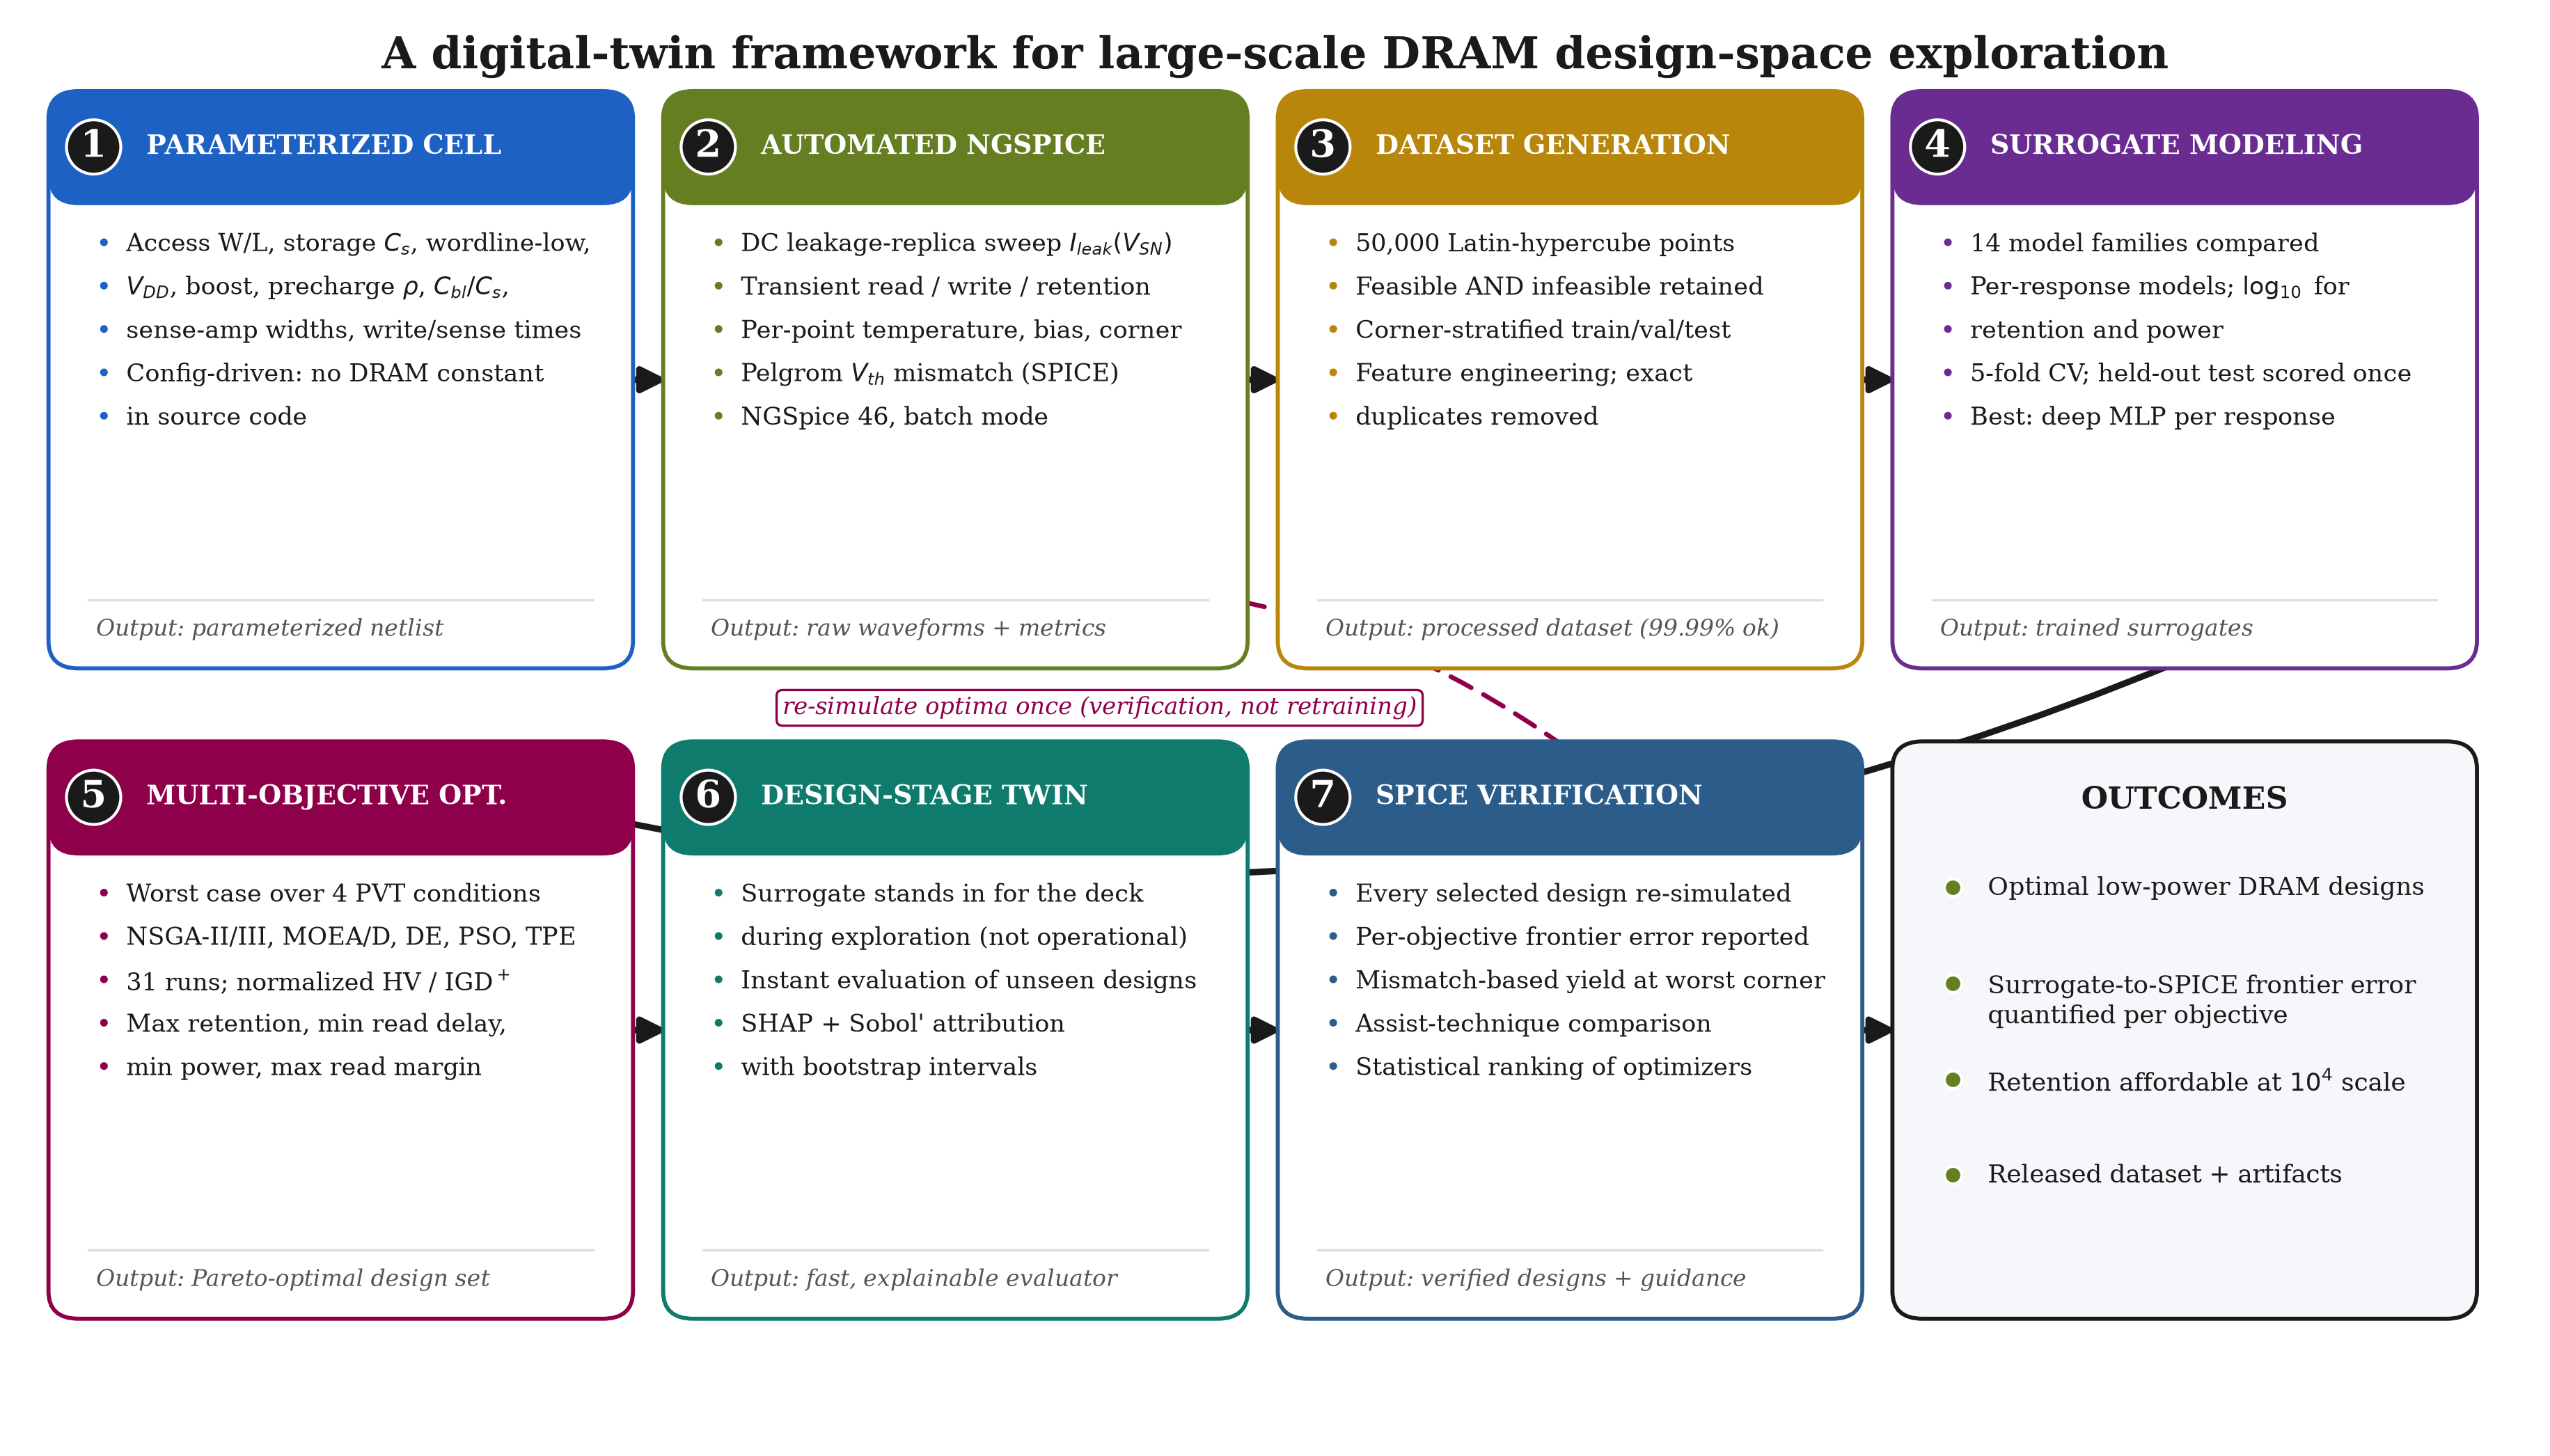
\includegraphics[width=\linewidth]{figures/fig01_framework.png}
\caption{Overview of the proposed framework. Stages one to three produce a
physically grounded dataset by automated SPICE characterization; stages four to
six convert it into a deployable digital twin and use that twin for robust
optimization; stage seven provides comparative and explanatory analysis. Optimizer
outputs are returned to the deck once for SPICE verification, not fed back into
training.}
\label{fig:framework}
\end{figure}

\subsection{The simulated slice}

Figure~\ref{fig:circuit} is the circuit each simulation evaluates.
Panel~(a) shows one 1T1C cell with its column periphery at transistor level: the
access device $M_{acc}$ connects bitline BL to storage node SN, the storage
capacitor $\Cs$ references a plate bias $V_{plate}$, each rail of the bitline pair
carries a lumped capacitance $\Cbl$, a CMOS transmission-gate write driver forces
BL to the data level, a precharge and equalize network restores both rails to
$\Vblpre$, and a cross-coupled NMOS/PMOS latch resolves the differential.
Panel~(b) shows the leakage replica: an access device identical to $M_{acc}$ whose
storage node is driven by the probe source $V_{snp}$, so a DC sweep of that source
yields $\Ileak(\Vsn)$ in the same deck.

Two features follow from physics rather than choice, both established by
simulation. The precharge pass devices are driven from a boosted rail VPP: with a
$V_{DD}$ gate and a $V_{DD}/2$ target the overdrive falls below threshold and the
rails cannot restore in time. Storing a full logic one requires
\begin{equation}
V_{\mathrm{PP}} > V_{DD} + V_{th,\mathrm{eff}},
\label{eq:vpp}
\end{equation}
where $V_{th,\mathrm{eff}}$ is the access-device threshold raised by the
storage-node body effect from its nominal $V_{th0}=\SI{0.62}{\volt}$ to about
\SI{0.85}{\volt}. It is $V_{th,\mathrm{eff}}$, not the full right-hand side, that
reaches \SI{0.85}{\volt}; with $V_{DD}$ swept to \SI{1.30}{\volt} the boosted rail
must clear $V_{DD}+V_{th,\mathrm{eff}}$, which is why the wordline-boost variable is
swept to \SI{1.2}{\volt}, spanning both the write-limited and fully-writing
regimes.

\begin{figure}[!ht]
\centering
\begin{subfigure}{\linewidth}\centering
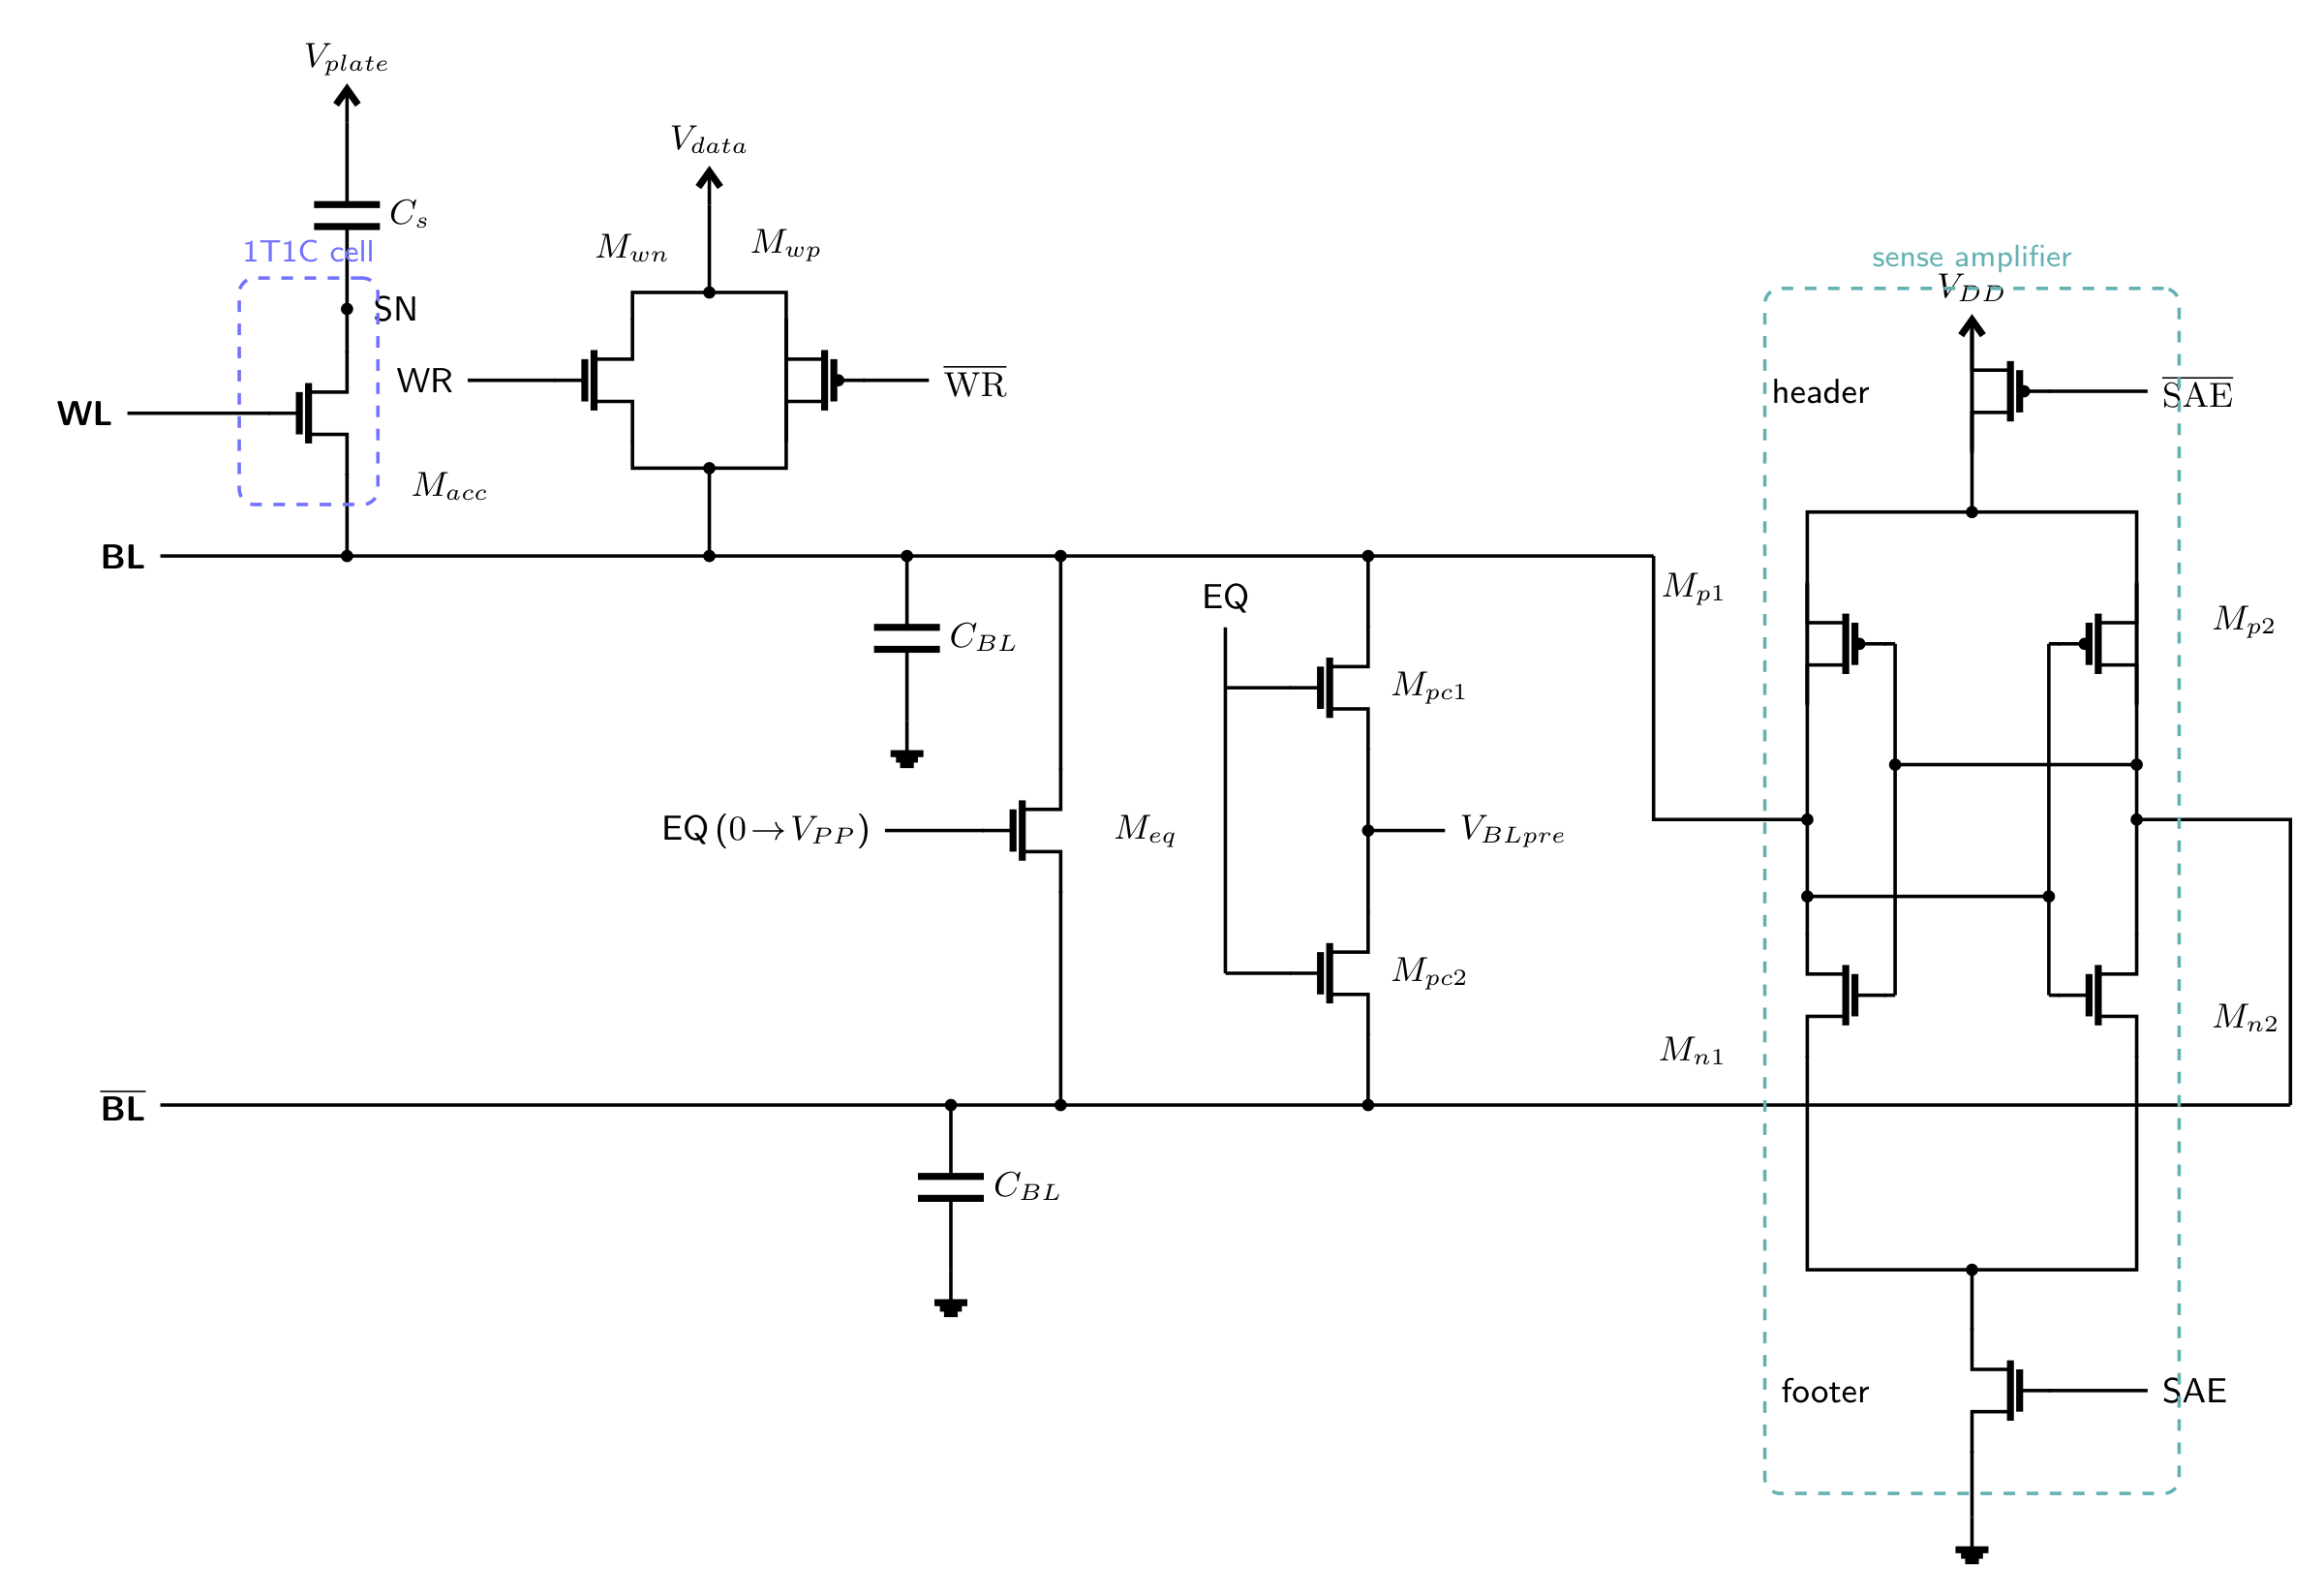
\includegraphics[width=0.96\linewidth]{figures/fig02_circuit.png}
\caption{Transistor-level schematic of the 1T1C cell and its column periphery;
the sense amplifier is a cross-coupled latch whose device gates tie to the
opposite rail.}
\label{fig:circuit-a}
\end{subfigure}\\[6pt]
\begin{subfigure}{0.60\linewidth}\centering
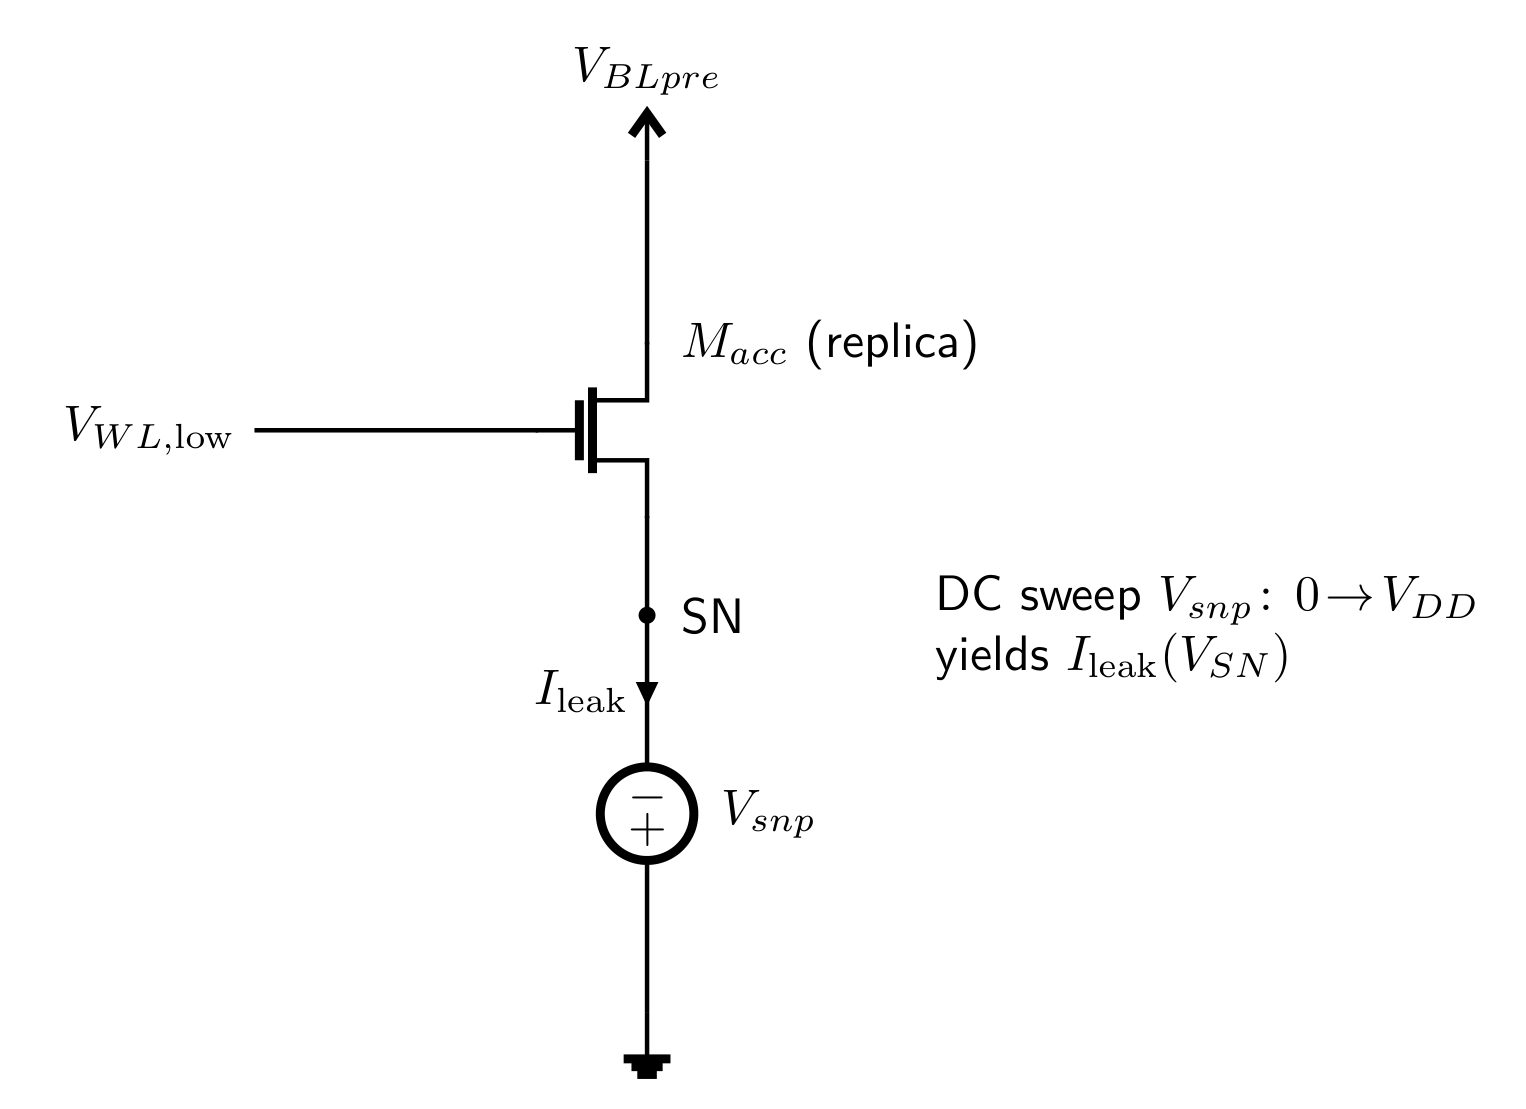
\includegraphics[width=\linewidth]{figures/fig02_replica.png}
\caption{Leakage replica: an access device identical to $M_{acc}$ probed by
$V_{snp}$ so that a DC sweep returns $\Ileak(\Vsn)$ in the same deck.}
\label{fig:circuit-b}
\end{subfigure}
\caption{The simulated DRAM slice, drawn in CircuiTikz with American source
symbols. (a) shows the cell and periphery and (b) the leakage replica.}
\label{fig:circuit}
\end{figure}

\subsection{The three-analysis deck}

Each design point is evaluated by one NGSpice invocation containing three
analyses (Algorithm~\ref{alg:spice}). An operating-point analysis of the idle
slice yields quiescent currents for standby power. A transient analysis executes
the sequence in Figure~\ref{fig:waveforms}: initial precharge, write of a logic
one, precharge, charge sharing, then sense with restore. Finally a DC sweep of the
replica probe yields the leakage characteristic. Figure~\ref{fig:waveforms}
captures a real transient rather than a drawing: (a) the control signals WL, PRE
and SAE; (b) the storage node charged to \SI{1.09}{\volt}, held through precharge,
falling to \SI{0.64}{\volt} on charge sharing and restored by the amplifier; and
(c) the bitline pair precharged to \SI{0.55}{\volt}, developing a
\SI{92}{\milli\volt} differential that the latch drives to the rails.

\begin{figure}[!ht]
\centering
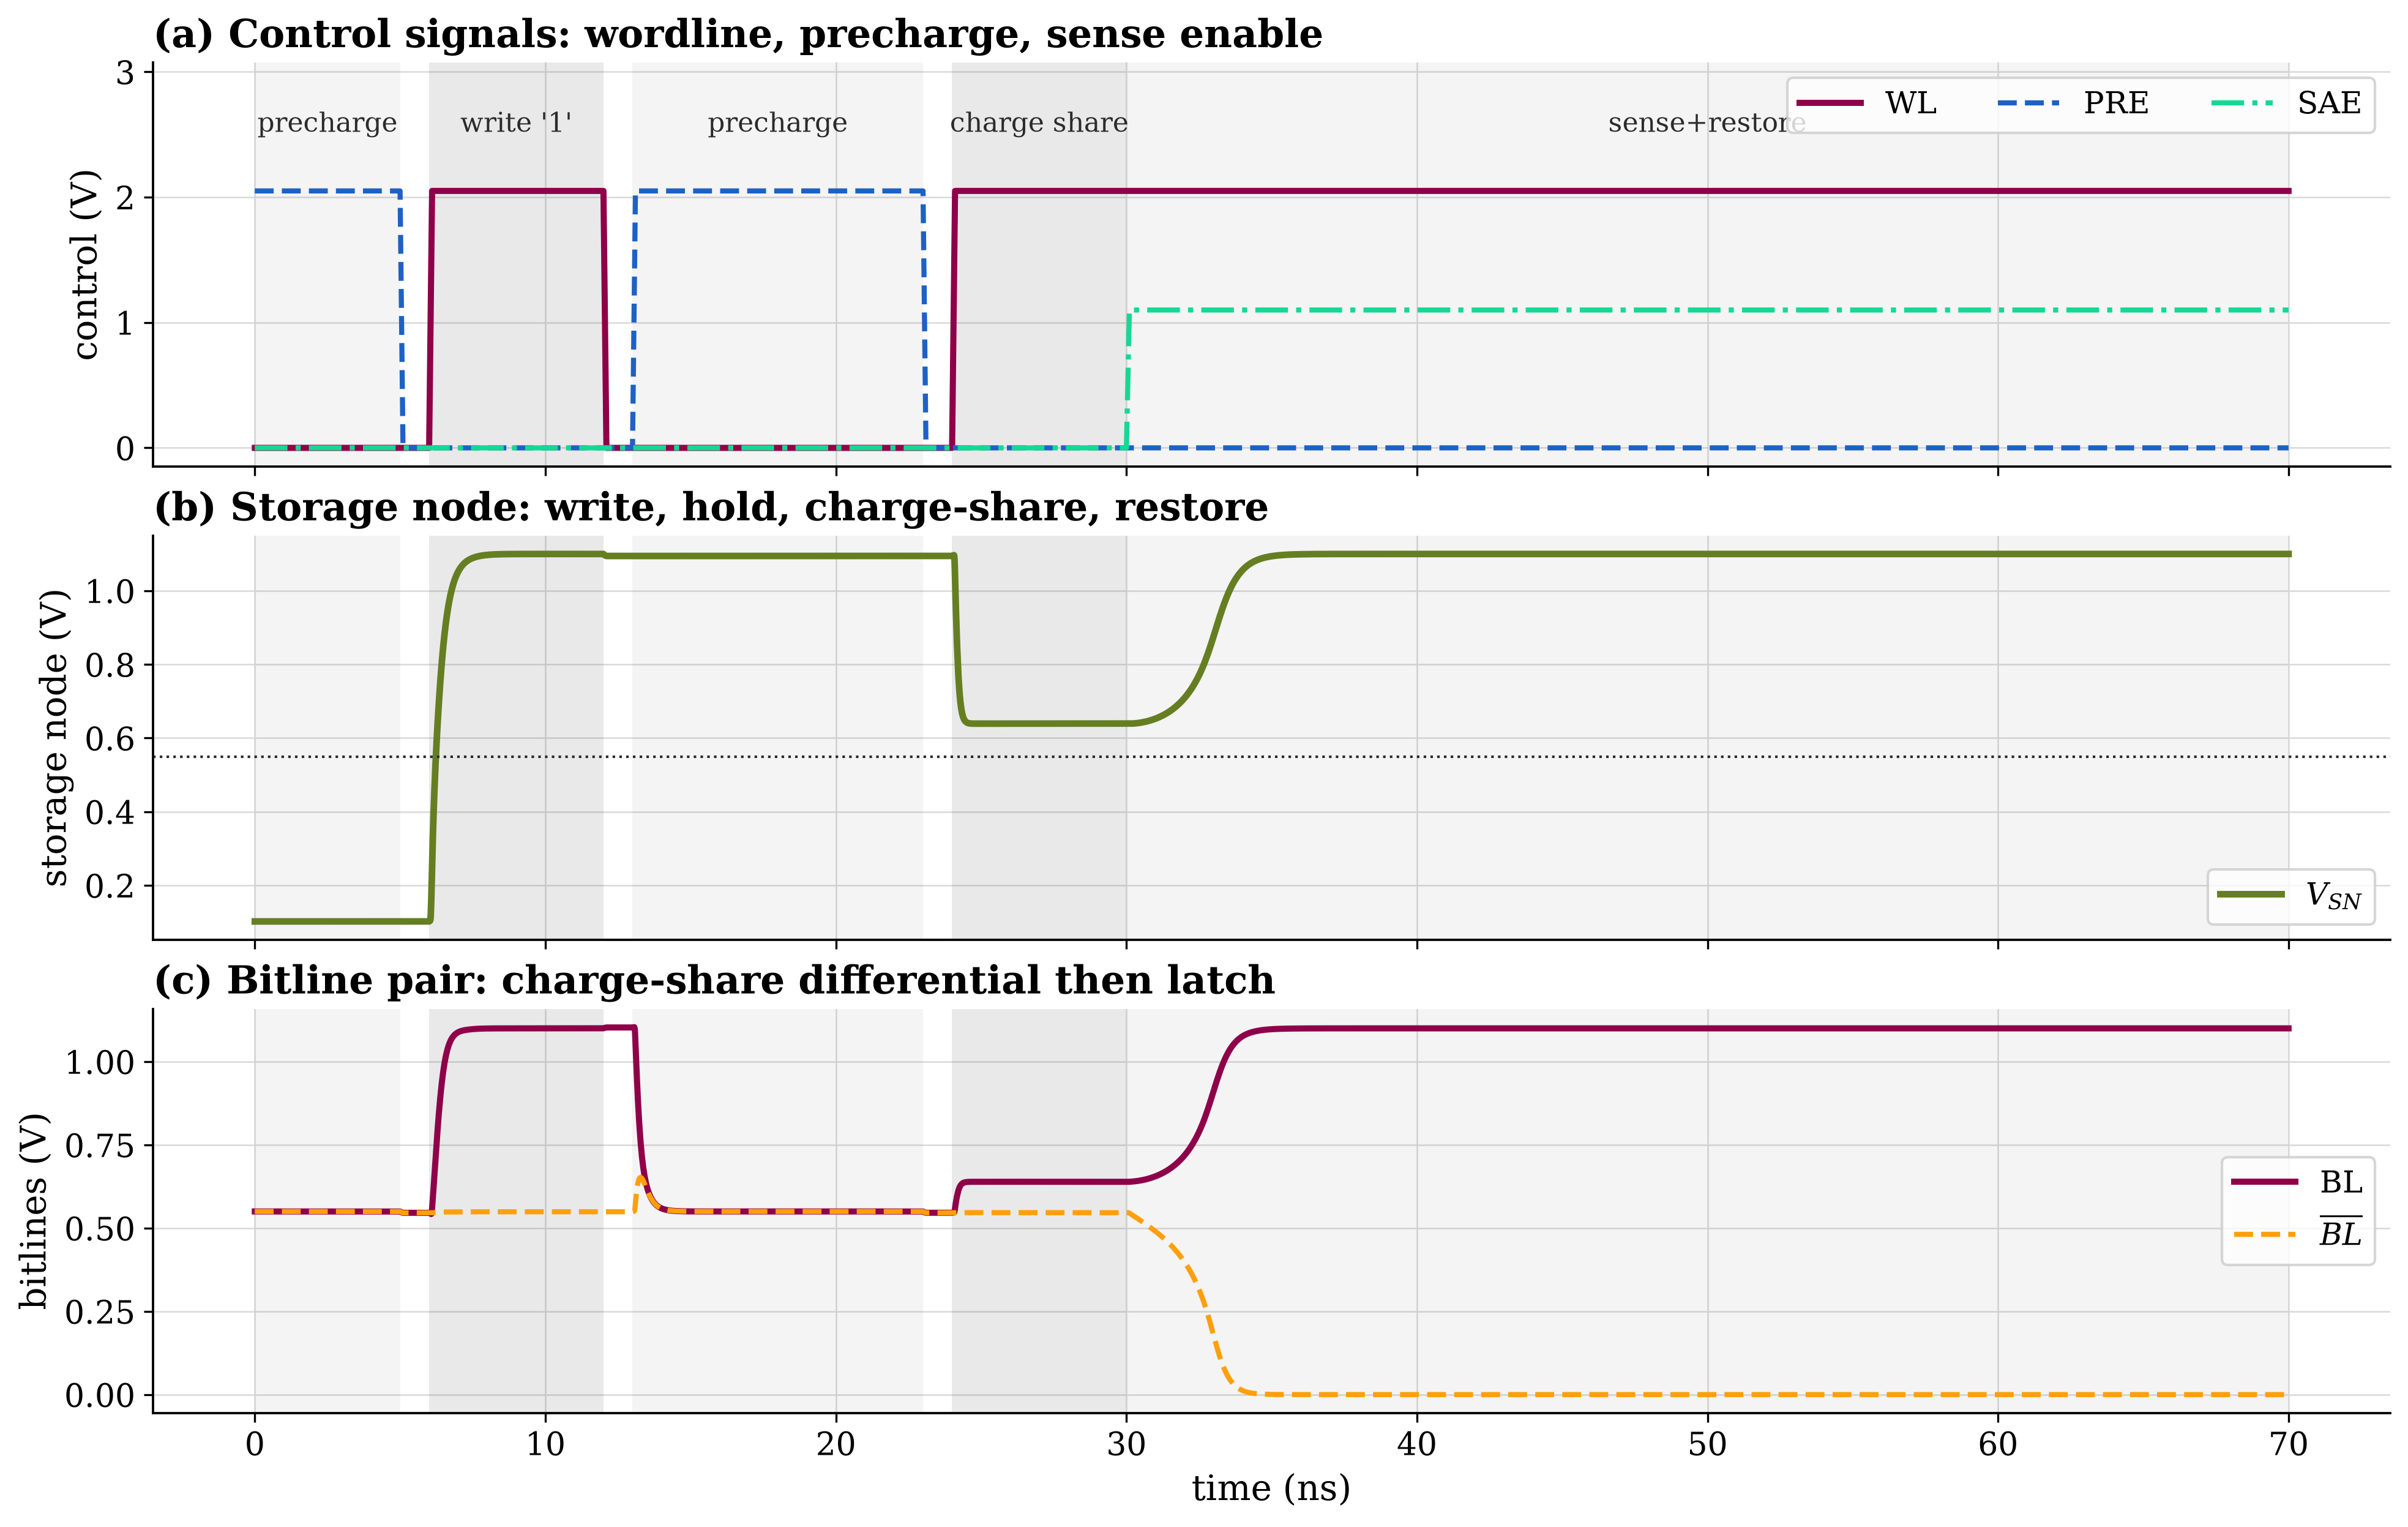
\includegraphics[width=0.92\linewidth]{figures/fig03_waveforms.png}
\caption{The characterization sequence, captured from a live NGSpice transient.
(a) Control signals: wordline WL, precharge enable PRE and sense-amplifier enable
SAE, with the five operation phases shaded, precharge, write of a logic one,
precharge, charge share, and sense with restore, over a \SI{70}{\nano\second}
window. (b) Storage node $\Vsn$ through the write, charge share and sense--restore;
the dotted line marks the plate bias. (c) The bitline pair; charge sharing produces
the differential that the latch resolves.}
\label{fig:waveforms}
\end{figure}

A single solver tolerance cannot serve all three analyses: the transient resolves
microampere currents while the leakage sweep resolves femtoampere currents.
Tolerances are therefore set per analysis, and the same holds with greater force
for \texttt{GMIN}, whose default of \SI{1e-12}{\siemens} injects hundreds of
femtoamperes across the storage-node junctions, far above the leakage measured.

\begin{algorithm}[!ht]
\caption{SPICE characterization of one DRAM design point}
\label{alg:spice}
\begin{algorithmic}[1]
\Require design point $\mathbf{p}$, technology $\mathcal{T}$, timing schedule
\Ensure measurements $\mathcal{M}$, leakage characteristic $\Ileak(\cdot)$
\State $\mathcal{C} \gets \mathcal{T}.\textsc{CardFor}(\mathbf{p}.\mathrm{corner})$
\State emit cell, bitline pair, precharge/equalize, write driver, sense latch
\State emit leakage replica: device identical to $M_{acc}$, node driven by
$V_{\mathrm{snp}}$
\State \textbf{Analysis 1 (operating point):} solve idle state; record
$i(V_{DD})$, $i(\Vblpre)$
\State set transient tolerances (\texttt{ABSTOL}$=10^{-13}$,
\texttt{GMIN}$=10^{-13}$)
\State \textbf{Analysis 2 (transient):} run schedule; measure
$\Vsn^{\mathrm{hold}}$, $t_{\mathrm{write}}$, $V_{BL}$, $V_{\overline{BL}}$,
$t_{\mathrm{read}}$, and $\int i_{DD}\,\mathrm{d}t$
\State set DC tolerances (\texttt{ABSTOL}$=10^{-18}$, \texttt{GMIN}$=10^{-15}$)
\State \textbf{Analysis 3 (DC sweep):} sweep $V_{\mathrm{snp}}: 0 \to V_{DD}$;
$\Ileak(V) \gets -\,i(V_{\mathrm{snp}})$
\State \Return $\mathcal{M}$, $\Ileak(\cdot)$
\end{algorithmic}
\end{algorithm}

\subsection{Extracted quantities}

Charge sharing between $\Cs$ and $\Cbl$ gives the bitline differential
\begin{equation}
\dVbl = \bigl(\Vsn - \Vblpre\bigr)\,\frac{\Cs}{\Cs + \Cbl},
\label{eq:chargeshare}
\end{equation}
used both as an independent check on the circuit and, inverted, to define the
retention failure level. The read margin and read delay are read from the sense
operation itself, not from Eq.~(\ref{eq:chargeshare}). The read margin is the fully
developed differential $v(\mathrm{bl})-v(\mathrm{blb})$ at the strobe time
$t_{\mathrm{sa}}$, after the cross-coupled latch has regenerated the small
charge-sharing signal; it therefore exceeds the pre-sense ceiling of
Eq.~(\ref{eq:chargeshare}) by the latch gain and is the differential a column
circuit actually resolves, which is why the constraint of \SI{25}{\milli\volt} is
placed on it rather than on $\dVbl$. The read delay is the interval from wordline
assertion to the latch crossing a fixed fraction of its rail. Both are measured on
the transient waveform and so carry the device nonlinearity that
Eq.~(\ref{eq:chargeshare}) omits. Access energy, Eq.~(\ref{eq:energy}), integrates
the supply currents over each window,
\begin{equation}
E_{\mathrm{read}} = V_{DD}\!\left|\int i_{DD}\,\mathrm{d}t\right|
+ \Vblpre\!\left|\int i_{\mathrm{pre}}\,\mathrm{d}t\right|,
\qquad
E_{\mathrm{access}} = \tfrac{1}{2}\bigl(E_{\mathrm{read}}+E_{\mathrm{write}}\bigr),
\label{eq:energy}
\end{equation}
with the absolute values taken because a supply-current sign reflects the source
reference, not the direction of energy flow. Power, Eq.~(\ref{eq:power}), decomposes into a
continuous leakage term, an access term proportional to the access rate, and a
refresh term inversely proportional to the refresh interval,
\begin{equation}
P_{\mathrm{total}} = P_{\mathrm{standby}}
+ E_{\mathrm{access}} f_{\mathrm{access}}
+ E_{\mathrm{read}} / t_{\mathrm{refresh}} .
\label{eq:power}
\end{equation}
The refresh term couples power directly to retention, which is why the two cannot
be treated as independent objectives. All three components are reported separately
so results can be reweighted for a different access profile without
re-simulation.

\subsection{Design of experiments}

The space is sampled by Latin hypercube sampling
\cite{mckay1979lhs,borisut2023alhs,phromphan2024lhs}, which guarantees one sample
per stratum in every one-dimensional projection: for $N$ samples in $d$
dimensions,
\begin{equation}
\bigl|\{\lfloor N u_{nj}\rfloor : n=1,\dots,N\}\bigr| = N
\quad \forall\, j\in\{1,\dots,d\}.
\label{eq:lhs}
\end{equation}
Each coordinate is decoded to its physical domain by its declared scale,
\begin{equation}
p_{nj} =
\begin{cases}
\ell_j + u_{nj}(h_j-\ell_j), & \text{linear},\\
\exp[\ln\ell_j + u_{nj}(\ln h_j - \ln\ell_j)], & \text{log},\\
c_{\lfloor u_{nj}|C_j|\rfloor}, & \text{categorical},
\end{cases}
\label{eq:decode}
\end{equation}
after which derived quantities are evaluated in declaration order, for example
$V_{\mathrm{PP}}=V_{DD}+V_{\mathrm{boost}}$, $\Vblpre=\rho V_{DD}$ and
$\Cbl=\kappa\Cs$ with $\rho,\kappa$ themselves sampled. Algorithm~\ref{alg:doe}
states the procedure.

\begin{algorithm}[!ht]
\caption{Configuration-driven sampling and decoding}
\label{alg:doe}
\begin{algorithmic}[1]
\Require design space $\mathcal{D}$, derived expressions $\mathcal{E}$, constants
$\mathcal{K}$, count $N$, master seed $\sigma$
\Ensure physical design points $\{\mathbf{p}^{(n)}\}$
\State $U \gets \textsc{LatinHypercube}(N,d,\textsc{DeriveSeed}(\sigma,\text{doe}))$
\Comment{Eq.~(\ref{eq:lhs})}
\State record centered-$L_2$ discrepancy and minimum pairwise distance
\For{$n \gets 1$ \textbf{to} $N$}
  \State $\mathbf{p}^{(n)} \gets \mathcal{K}$;
  \ $p^{(n)}_j \gets \textsc{Decode}(u_{nj})\ \forall j$
  \Comment{Eq.~(\ref{eq:decode})}
  \State evaluate each $e\in\mathcal{E}$ in declaration order
\EndFor
\State \Return $\{\mathbf{p}^{(n)}\}$
\end{algorithmic}
\end{algorithm}

\subsection{Process corners and mismatch}

The Predictive Technology Model gives one typical card per node
\cite{zhao2006ptm}. Slow/fast corners are synthesized by first-order shifts,
\begin{equation}
V_{th0}' = V_{th0} + \mathrm{sgn}(V_{th0})\,\Delta V_{th0},
\quad u_0' = \alpha u_0,
\quad t_{ox}' = \beta t_{ox},
\label{eq:corner}
\end{equation}
where the shift acts on the \emph{magnitude} of each device threshold: a positive
$\Delta V_{th0}$ slows the device by enlarging $|V_{th0}|$ and a negative value
speeds it, the device polarity $\mathrm{sgn}(V_{th0})$ merely steering the shift so
one table entry has the intended effect on both NMOS and PMOS.
Table~\ref{tab:corners} states the four synthesized corners in full; TT is the
unmodified card. Local mismatch uses the Pelgrom model
\cite{pelgrom1989matching},
\begin{equation}
\sigma_{V_{th}} = \frac{A_{VT}}{\sqrt{W L}},
\label{eq:pelgrom}
\end{equation}
applied per device through the BSIM4 instance parameter \texttt{delvto}.
Equation~(\ref{eq:corner}) shifts every device in a sample together (global
variation) while Eq.~(\ref{eq:pelgrom}) perturbs each independently (local
mismatch).

\begin{table}[!ht]
\centering
\caption{The four synthesized process corners. $\Delta V_{th0}$ is the shift added
to $|V_{th0}|$ ($+$ slower, $-$ faster); $u_0$ and $t_{ox}$ entries are
multiplicative. TT is the unmodified PTM card. The recipe is first-order and is not
a foundry-signed-off corner model.}
\label{tab:corners}
\footnotesize
\begin{tabular}{@{}l ccc c ccc@{}}
\toprule
& \multicolumn{3}{c}{\textbf{NMOS}} & & \multicolumn{3}{c}{\textbf{PMOS}} \\
\cmidrule(lr){2-4}\cmidrule(lr){6-8}
\textbf{Corner} & $\Delta|V_{th0}|$ & $u_0$ & $t_{ox}$ & &
$\Delta|V_{th0}|$ & $u_0$ & $t_{ox}$ \\
\midrule
TT & --          & 1.00 & 1.00 & & --          & 1.00 & 1.00 \\
SS & $+45$\,mV    & 0.95 & 1.02 & & $+45$\,mV    & 0.95 & 1.02 \\
FF & $-45$\,mV    & 1.05 & 0.98 & & $-45$\,mV    & 1.05 & 0.98 \\
SF & $+45$\,mV    & 0.95 & 1.00 & & $-45$\,mV    & 1.05 & 1.00 \\
FS & $-45$\,mV    & 1.05 & 1.00 & & $+45$\,mV    & 0.95 & 1.00 \\
\bottomrule
\end{tabular}
\end{table}

%=======================================================================
\section{Quasi-Static Retention Modeling}
\label{sec:retention}

\subsection{Formulation}

Once the wordline is low, the storage node is an isolated capacitor, so charge
conservation is exact,
\begin{equation}
\Cnode\,\frac{\mathrm{d}\Vsn}{\mathrm{d}t} = -\,\Ileak(\Vsn).
\label{eq:ode}
\end{equation}
Equation~(\ref{eq:ode}) involves no approximation; the entire difficulty of
retention is that integrating it in time needs a ten-decade transient. Because
$\Ileak$ depends only on $\Vsn$, the equation is separable, and integrating
between the written level and the failure level eliminates time and gives
retention in closed form,
\begin{equation}
\boxed{\;
\tret = \int_{\Vfail}^{V_{\mathrm{init}}}
\frac{\Cnode}{\Ileak(V)}\,\mathrm{d}V \;}
\label{eq:tret}
\end{equation}
Equation~(\ref{eq:tret}) carries one physical assumption, that leakage is
quasi-static, which holds because the discharge is far slower than every device
time constant, together with one modeling boundary: $\Ileak$ is the current the
access-device compact model reports, so every mechanism that model describes is
included, while dielectric leakage of the storage capacitor, for which the deck
carries no compact model, is not. Retention here is therefore an
access-device-limited estimate. Within that boundary the method assumes nothing
about the magnitude or dominant mechanism of leakage, both of which are measured
rather than posited. The failure level is derived from the sense-margin
specification rather than assumed directly: a cell fails when charge sharing can no
longer resolve a differential, so setting $\dVbl=\dVmin$ in
Eq.~(\ref{eq:chargeshare}) gives
\begin{equation}
\Vfail = \Vblpre + \dVmin\,\frac{\Cs+\Cbl}{\Cs},
\qquad
t_{\mathrm{refresh}} = \tret / \gamma ,
\label{eq:vfail}
\end{equation}
with $\gamma$ a policy guard band. The refresh interval booked against a design is
thus $\tret/\gamma$; at the $\gamma=2$ used throughout, sustaining the JEDEC
\SI{64}{\milli\second} refresh interval requires $\tret\ge\SI{128}{\milli\second}$,
whereas the yield criterion of \S\ref{sec:results} applies the weaker floor
$\tret\ge\SI{64}{\milli\second}$, that is, the bit survives at least one nominal
refresh period. If $V_{\mathrm{init}}\le\Vfail$ the write already fails and
$\tret=0$, a real observation rather than a missing value; if $\Ileak$ falls to the
leakage floor $\epsilon_I=\SI{1e-21}{\ampere}$ anywhere in the range, a numerical
guard against division by zero that the node's leakage never physically reaches,
the node holds the bit indefinitely within that bias condition and the observation
is right-censored. This floor test, $\min\Ileak\le\epsilon_I$, is the condition
applied in Algorithm~\ref{alg:retention}.

\subsection{What is measured}

The DC sweep supplies $\Ileak(\Vsn)$ containing every mechanism the access-device
compact model describes,
\begin{equation}
\Ileak(\Vsn) = I_{\mathrm{sub}} + I_{\mathrm{GIDL}}
+ I_{\mathrm{junc}} + I_{\mathrm{gate}} .
\label{eq:leakcomp}
\end{equation}
The card enables gate tunneling, the junction diode model and non-zero GIDL
coefficients, so no access-device term is omitted. The method does not need the terms separated,
since the sweep returns their sum, exactly what Eq.~(\ref{eq:tret}) requires;
Eq.~(\ref{eq:leakcomp}) matters because it confirms nothing is excluded and
explains the measured shape. The subthreshold and GIDL terms have the familiar
forms
\begin{align}
I_{\mathrm{sub}} &\propto
\exp\!\Big(\tfrac{V_{gs}-V_{th}}{n k_BT/q}\Big)
\Big[1-\exp\!\big(-\tfrac{V_{ds}}{k_BT/q}\big)\Big],
\label{eq:isub}\\
I_{\mathrm{GIDL}} &= A_{\mathrm{GIDL}} W\,
\frac{V_{ds}-V_{gs}-E_{\mathrm{GIDL}}}{t_{ox}}
\exp\!\Big(\tfrac{-B_{\mathrm{GIDL}} t_{ox}}{V_{ds}-V_{gs}-E_{\mathrm{GIDL}}}\Big),
\label{eq:igidl}
\end{align}
the second of which explains why a negative wordline is not unambiguously good:
driving $V_{gs}$ negative suppresses Eq.~(\ref{eq:isub}) but raises the numerator
and exponent of Eq.~(\ref{eq:igidl}).

Figure~\ref{fig:retention} presents the measured characteristic and the model
validation. Panel~(a) gives $\Ileak(\Vsn)$ at six temperatures. Panel~(b) plots
the leakage at the written level against $1/k_BT$. Above about \SI{55}{\celsius}
it rises steeply with an extracted activation energy of \SI{1.31}{\electronvolt},
close to the silicon bandgap and therefore consistent with diffusion-limited
junction leakage where $n_i^2\propto\exp(-E_g/k_BT)$; this hot, thermally
activated regime is where retention is set. Below room temperature the curve
flattens, but that plateau is not physical: at the campaign solver floor
(DC $\texttt{GMIN}=10^{-15}\,\mathrm{S}$) it sits at \SI{1.6}{\femto\ampere}, and
the $\texttt{GMIN}$ sweep of panel~(f) shows this value tracking $1/\texttt{GMIN}$
rather than any device parameter, the ohmic signature $k/\texttt{GMIN}\approx1.2$
of the solver's minimum-conductance injection. Converging the floor to
$10^{-17}\,\mathrm{S}$ lowers the cold leakage to \SI{0.56}{\femto\ampere}; at
\SI{125}{\celsius}, by contrast, $k/\texttt{GMIN}=5.9\times10^{3}$ and the leakage
is unchanged to within 2\%, so the design-relevant hot corner is physical and
floor-independent. Panel~(c) shows the integrand $\Cnode/\Ileak$ of
Eq.~(\ref{eq:tret}), whose area is the retention time; retention runs from tens of
seconds at the cold, floor-limited end to \SI{1.9}{\milli\second} at
\SI{125}{\celsius}. Panels~(d) and~(e) validate the model across its full working
range: pooling 200 short-retention points with 30 points carried out to
\SI{25}{\second} by coarse-step transient integration (Table~\ref{tab:retval}),
the quasi-static prediction matches direct transient simulation with $r=0.99992$
over roughly six and a half decades, 100\% within a factor of two, and a median
error of $-0.011$ decades. The slight systematic under-prediction is consistent
with neglecting the voltage-dependent parasitic capacitance of the access device.

The numerical floor touches only the cold end, and no reported result depends on
it. The retention objective is worst-cased over the conditions $\mathcal{Q}$,
whose binding member is always the hot corner (\SI{0.13}{\second} at
\SI{85}{\celsius}, \SI{1.9}{\milli\second} at \SI{125}{\celsius}), orders of
magnitude below the cold values; and the \SI{64}{\milli\second} criterion is met
at \SI{27}{\celsius} with wide margin whether the cold leakage reads \num{0.56} or
\SI{1.6}{\femto\ampere}. The floor is therefore bounded, labelled and non-binding
rather than removed at the cost of regenerating the entire campaign.

\begin{figure}[!ht]
\centering
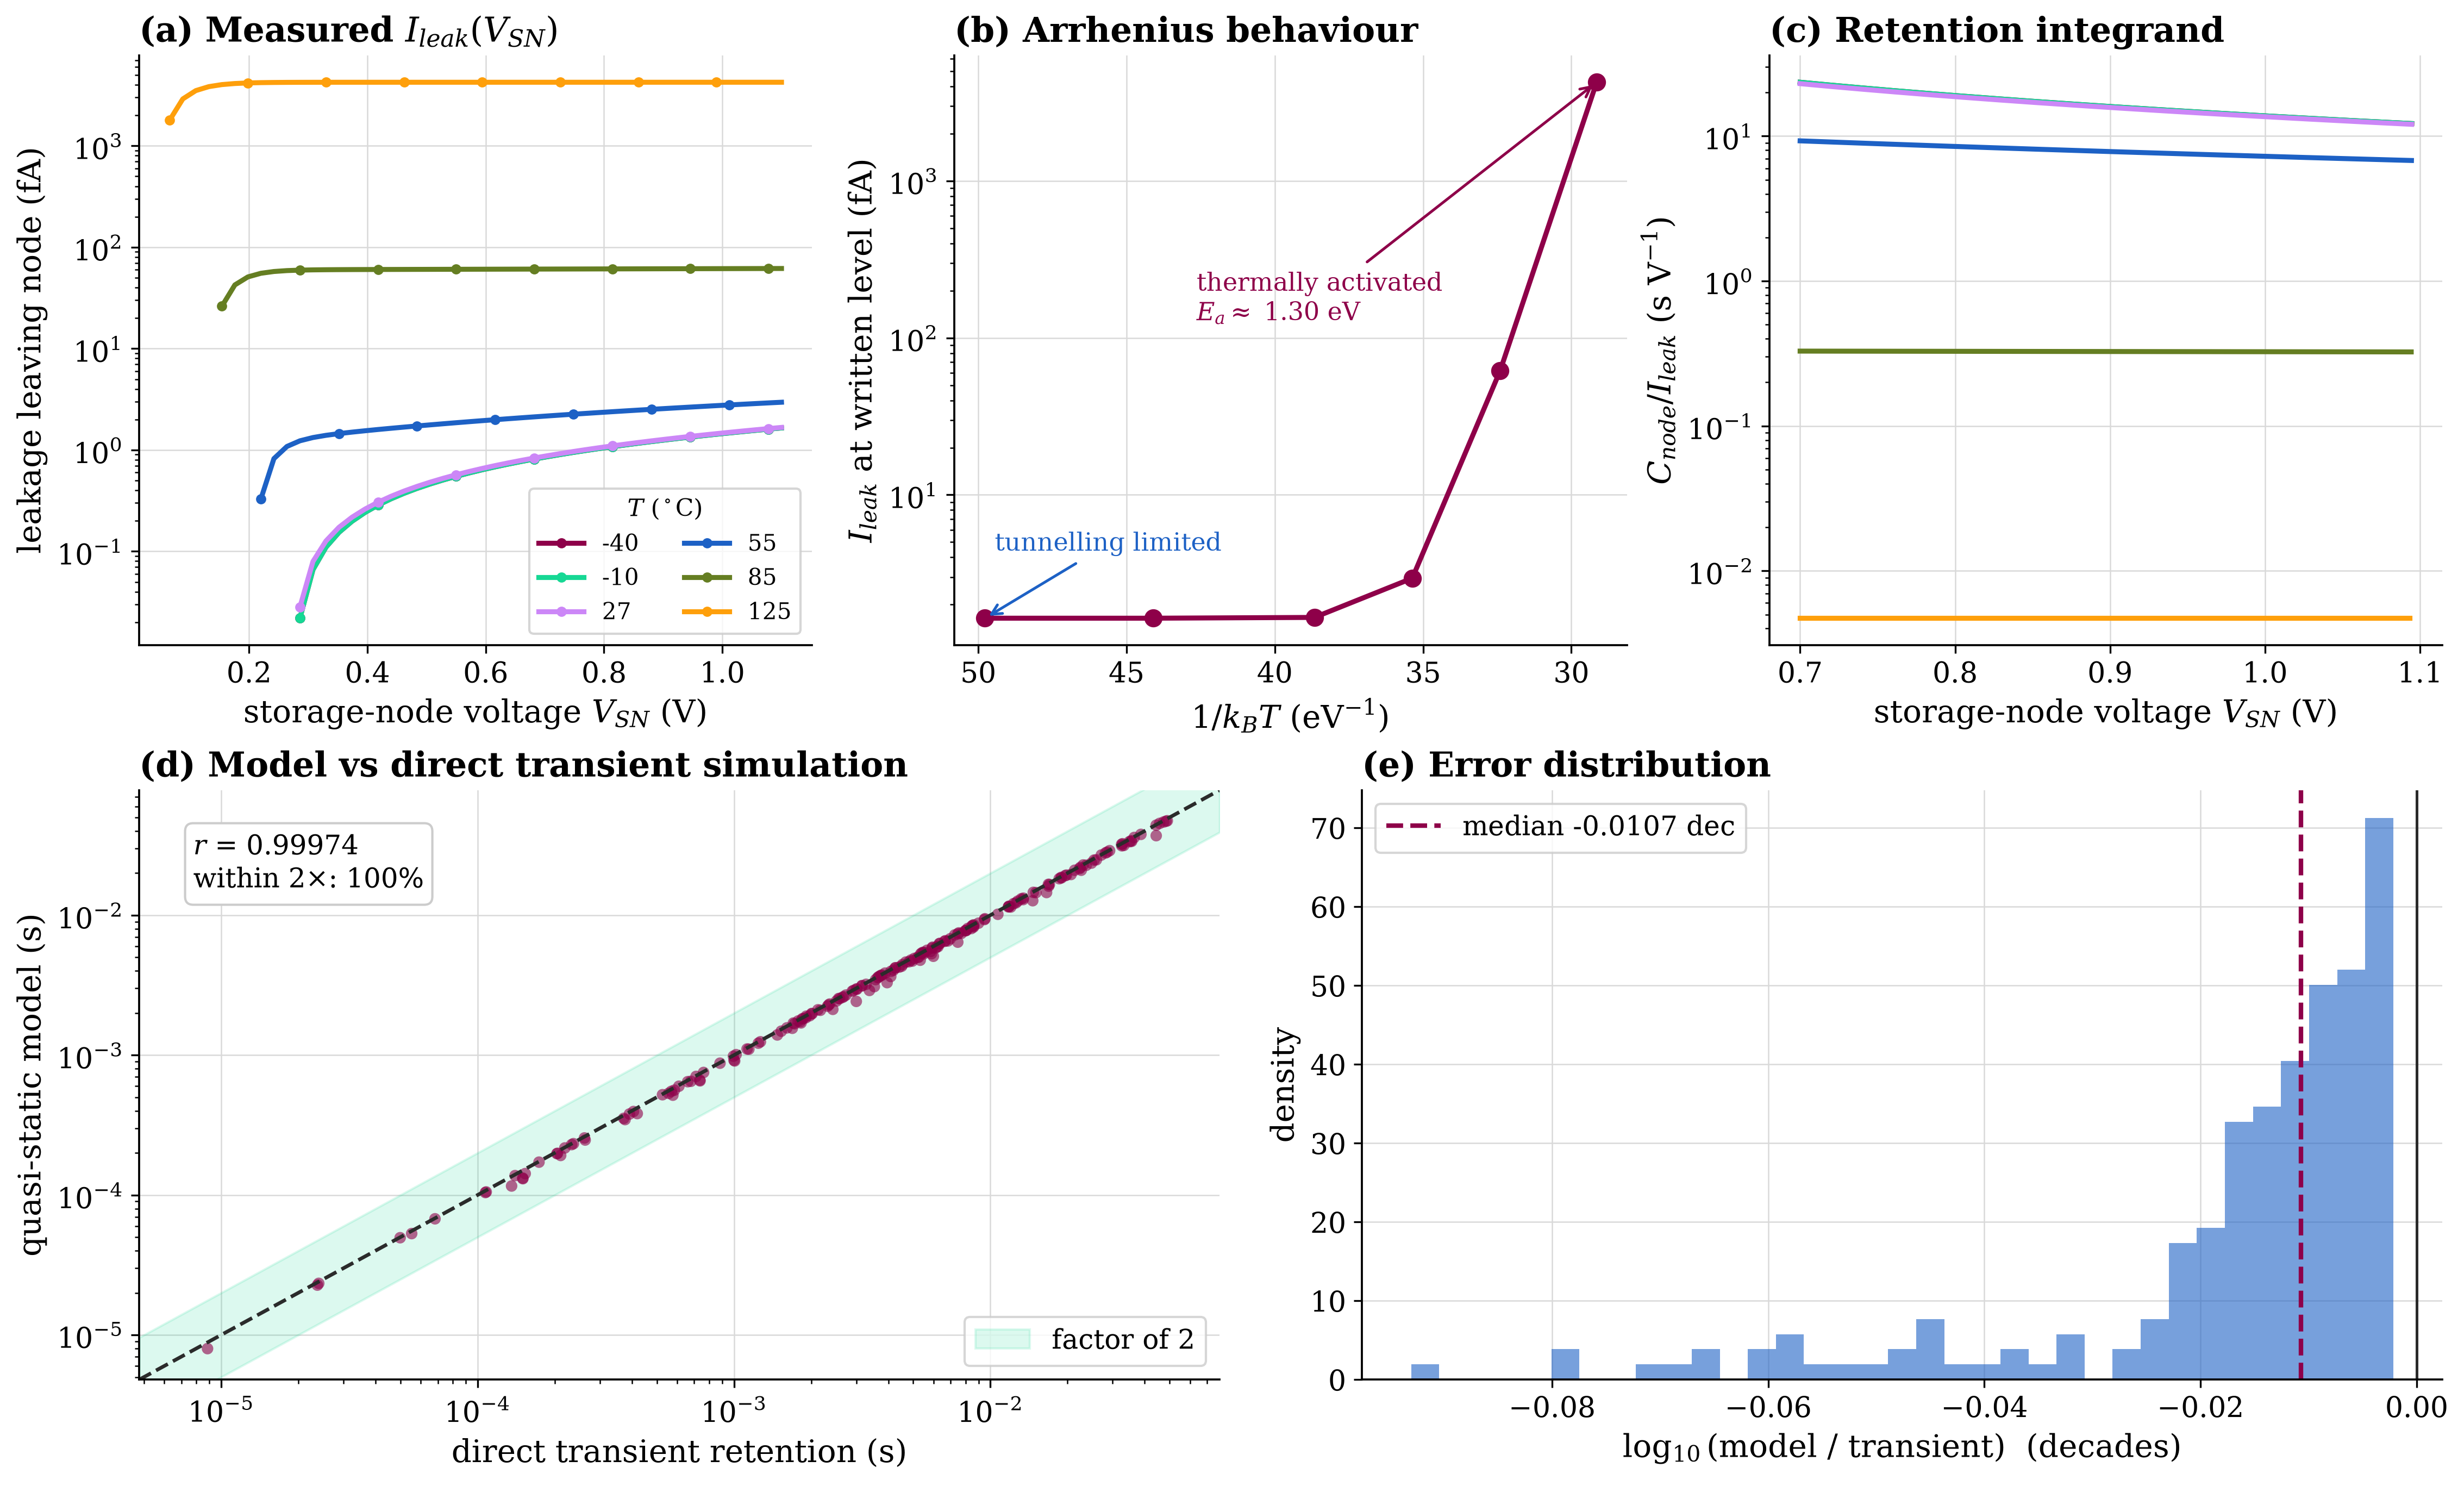
\includegraphics[width=\linewidth]{figures/fig04_retention.png}
\caption{Measured storage-node leakage and validation of the quasi-static model.
(a) $\Ileak(\Vsn)$ at six temperatures at the converged floor. (b) Leakage at the
written level against $1/k_BT$: a thermally activated regime with
$E_a\approx\SI{1.31}{\electronvolt}$ and a low-temperature plateau set by the
solver floor rather than the device (see~(f)). (c) The retention integrand
$\Cnode/\Ileak$ of Eq.~(\ref{eq:tret}). (d) Quasi-static prediction against direct
transient simulation over the full working range, short points plus a
long-retention set out to \SI{25}{\second}; the shaded band is a factor of two.
(e) Distribution of the $\log_{10}$ ratio between the two. (f) Convergence of the
written-level leakage as DC $\texttt{GMIN}$ is swept from $10^{-14}$ to
$10^{-18}\,\mathrm{S}$: the cold curves track $1/\texttt{GMIN}$ (numerical), the
\SI{125}{\celsius} curve is flat (physical).}
\label{fig:retention}
\end{figure}

\begin{table}[!ht]
\centering
\caption{Quasi-static retention against direct transient simulation, matched on
identical designs, split by retention range. The pooled set spans the model's full
working range.}
\label{tab:retval}
\footnotesize
\begin{tabular}{@{}lccccc@{}}
\toprule
\textbf{Range} & \textbf{$n$} & \textbf{$r_{\log_{10}}$} &
\textbf{median err (dec)} & \textbf{$p_{90}|$err$|$ (dec)} & \textbf{within $2\times$} \\
\midrule
short ($\approx$9\,\textmu s--49\,ms) & 200 & 0.99974 & $-0.0107$ & 0.044 & 100\% \\
long (1.05--25.2\,s)                  & 30  & 0.99980 & $-0.0077$ & 0.021 & 100\% \\
\midrule
pooled ($\approx$6.5 decades)         & 230 & 0.99992 & $-0.0106$ & 0.037 & 100\% \\
\bottomrule
\end{tabular}
\end{table}

Algorithm~\ref{alg:retention} states the computation: the integral is evaluated by
trapezoidal quadrature on a uniform grid, adequate because $\Ileak$ is smooth and
strictly positive over the range whenever the design is feasible.

\begin{algorithm}[!ht]
\caption{Quasi-static retention from measured leakage}
\label{alg:retention}
\begin{algorithmic}[1]
\Require $\Ileak(\cdot)$, $\Cnode$, $V_{\mathrm{init}}$, $\Vblpre$, $\Cs$, $\Cbl$,
$\dVmin$, grid $N_g$, leakage floor $\epsilon_I=\SI{1e-21}{\ampere}$
\Ensure retention $\tret$ and censoring flag
\State $\Vfail \gets \Vblpre + \dVmin(\Cs+\Cbl)/\Cs$
\Comment{Eq.~(\ref{eq:vfail})}
\If{$V_{\mathrm{init}} \le \Vfail$} \Return $\tret \gets 0$ (not censored)
\EndIf
\State $\mathcal{V} \gets$ grid of $N_g$ points on $[\Vfail,V_{\mathrm{init}}]$;
$I \gets \textsc{Interp}(\Ileak,\mathcal{V})$
\If{$\min I \le \epsilon_I$} \Return $\tret \gets \infty$ (censored)
\EndIf
\State \Return $\tret \gets \textsc{Trapezoid}(\Cnode/I,\mathcal{V})$
\Comment{Eq.~(\ref{eq:tret})}
\end{algorithmic}
\end{algorithm}

%=======================================================================
\section{Experimental Setup}
\label{sec:setup}

Table~\ref{tab:designspace} lists the 15 sampled variables; thirteen are design
variables and two are operating conditions treated separately during
optimization. Table~\ref{tab:setup} states the technology and solver
configuration.

\begin{table}[!ht]
\centering
\caption{The sampled design space. Thirteen design variables plus two operating
conditions.}
\label{tab:designspace}
\footnotesize
\begin{tabular}{@{}llrrll@{}}
\toprule
\textbf{Variable} & \textbf{Group} & \textbf{Lower} & \textbf{Upper} &
\textbf{Unit} & \textbf{Scale} \\
\midrule
$V_{DD}$              & design      & 0.70   & 1.30   & V   & linear \\
$V_{\mathrm{boost}}$  & design      & 0.30   & 1.20   & V   & linear \\
$V_{WL,\mathrm{low}}$ & design      & $-0.40$& 0.00   & V   & linear \\
$\rho$ (BL precharge) & design      & 0.35   & 0.65   & 1   & linear \\
$\Cs$                 & design      & 5.0    & 40.0   & fF  & log \\
$\kappa$ ($\Cbl/\Cs$) & design      & 2.0    & 12.0   & 1   & linear \\
$W_{\mathrm{acc}}$    & design      & 60     & 220    & nm  & linear \\
$L_{\mathrm{acc}}$    & design      & 45     & 120    & nm  & linear \\
$W_{\mathrm{san}}$    & design      & 90     & 540    & nm  & log \\
$W_{\mathrm{sap}}/W_{\mathrm{san}}$ & design & 1.0 & 3.0 & 1 & linear \\
$W_{\mathrm{en}}/W_{\mathrm{san}}$  & design & 1.0 & 4.0 & 1 & linear \\
$t_{\mathrm{wr}}$     & design      & 1.0    & 10.0   & ns  & linear \\
$t_{\mathrm{sense}}$  & design      & 1.0    & 10.0   & ns  & linear \\
$T$                   & condition   & $-40$  & 125    & \si{\celsius} & linear \\
corner                & condition   & \multicolumn{3}{l}{\{TT, SS, FF, SF, FS\}} & set \\
\bottomrule
\end{tabular}
\end{table}

\begin{table}[!ht]
\centering
\caption{Technology, solver and campaign configuration.}
\label{tab:setup}
\footnotesize
\begin{tabular}{@{}ll@{}}
\toprule
\textbf{Item} & \textbf{Value} \\
\midrule
Simulator & NGSpice 46 (console build), batch mode \cite{ngspice} \\
Device models & PTM BSIM4 level 54, 45\,nm low-power \cite{zhao2006ptm} \\
Enabled leakage physics & gate tunneling, junction diode, non-zero GIDL \\
Corners & TT/SS/FF/SF/FS; $\Delta V_{th0}=\pm\SI{45}{\milli\volt}$,
$u_0(1\pm0.05)$, $t_{ox}(1\mp0.02)$ \\
Transient tolerances & \texttt{ABSTOL}$=10^{-13}$, \texttt{GMIN}$=10^{-13}$ \\
DC tolerances & \texttt{ABSTOL}$=10^{-18}$, \texttt{GMIN}$=10^{-15}$ \\
Sense offset $\dVmin$ / refresh guard $\gamma$ & \SI{25}{\milli\volt} / 2.0 \\
Sampler & Latin hypercube, $N=50{,}000$, $d=15$ \\
Master seed / configuration hash & 20260723 / \texttt{954478d4cad7f9d6} \\
Parallelism & 18 worker processes \\
\bottomrule
\end{tabular}
\end{table}

Table~
ef{tab:config} lists the objectives, constraints, operating
conditions and load-bearing constants, and Table~
ef{tab:nomen} the
principal symbols; no value used below is left implicit.

% ===== Configuration table (M14) =====
\begin{table}[!ht]
\centering
\caption{Objectives, constraints, operating conditions and the load-bearing
constants of the study, complementing the technology and solver settings of
Table~\ref{tab:setup} and the variables of Table~\ref{tab:designspace}. Every
value is an explicit configuration entry, not a hidden constant; together the
three tables and the released configuration reproduce each result.}
\label{tab:config}
\footnotesize
\begin{tabular}{@{}lll@{}}
\toprule
\textbf{Symbol / item} & \textbf{Value} & \textbf{Role} \\
\midrule
\multicolumn{3}{@{}l@{}}{\textit{Objectives (worst case over the conditions $\mathcal{Q}$)}}\\
$\tret$ (retention) & maximize ($\log_{10}$) & Eqs.~(\ref{eq:ode})--(\ref{eq:tret}) \\
$t_{rd}$ (read delay) & minimize & timing budget \\
$P_{\mathrm{total}}$ (power) & minimize ($\log_{10}$) & Eq.~(\ref{eq:power}) \\
read margin & maximize & developed SA differential \\
\addlinespace
\multicolumn{3}{@{}l@{}}{\textit{Constraints (thresholds $\tau_s$)}}\\
read margin & $\ge \SI{25}{\milli\volt}$ & exceeds SA offset \\
write efficiency & $\ge 0.85$ & $\Vsn/V_{DD}$ \\
read delay & $\le \SI{30}{\nano\second}$ & inside timing budget \\
retention (yield spec) & $\ge \SI{64}{\milli\second}$ & JEDEC refresh budget \\
\addlinespace
\multicolumn{3}{@{}l@{}}{\textit{Operating conditions $\mathcal{Q}$ (4 PVT points)}}\\
$\mathcal{Q}$ & \{(27,TT),(85,SS),(125,SS),(85,FF)\} & ($^\circ$C, corner) \\
\addlinespace
\multicolumn{3}{@{}l@{}}{\textit{Physical / metric constants}}\\
$\dVmin$ & \SI{25}{\milli\volt} & sense offset + guard (Eq.~\ref{eq:vfail}) \\
$\gamma$ (refresh guard) & 2.0 & $t_{\mathrm{refresh}}=\tret/\gamma$ \\
$f_{\mathrm{access}}$ & \SI{1e5}{\hertz} & active-power access rate \\
$\Cnode$ & $\Cs$ (+overhead $0$) & storage-node capacitance \\
$V_{\mathrm{plate}}$ & $\rho V_{DD}$ ($\approx\SI{0.55}{\volt}$ nom.) & cell-plate bias \\
$V_{\mathrm{init}}$ & $\Vsn^{\mathrm{hold}}$ (written level) & integration upper limit \\
retention grid $N_g$ & 2001 & quadrature points \\
leakage floor $\epsilon_I$ & \SI{1e-21}{\ampere} & censoring guard (Alg.~\ref{alg:retention}) \\
log floor $\epsilon_t$ & \SI{1e-12}{\second} & floors $\tret$ before $\log_{10}$ \\
\addlinespace
\multicolumn{3}{@{}l@{}}{\textit{Selection and mismatch}}\\
selection weights & [0.30, 0.25, 0.30, 0.15] & ret/delay/power/margin \\
$A_{VT}$ (Pelgrom) & \SI{3.5}{\milli\volt\micro\metre} & Eq.~(\ref{eq:pelgrom}) \\
mismatch $\sigma_{V_{th}}$ & $A_{VT}/\sqrt{WL}$, per device & Eq.~(\ref{eq:pelgrom}) \\
process sigmas & $\sigma_{\Cs}{=}\sigma_{\Cbl}{=}0.05$; $\sigma_W{=}0.04$; & robustness \\
 & $\sigma_{V_{DD}}{=}\sigma_{V}{=}0.02$ & (relative) \\
\addlinespace
\multicolumn{3}{@{}l@{}}{\textit{Analysis}}\\
Sobol' base $N$ & 2048; $B{=}500$ bootstrap & \cite{saltelli2010sobol} \\
SHAP estimator & Kernel/Deep SHAP \cite{lundberg2017shap} & neural twin \\
\bottomrule
\end{tabular}
\end{table}

% ===== Nomenclature (L9) =====
\begin{table}[!ht]
\centering
\caption{Nomenclature of the principal symbols.}
\label{tab:nomen}
\footnotesize
\begin{tabular}{@{}ll@{\hskip 24pt}ll@{}}
\toprule
\textbf{Symbol} & \textbf{Meaning} & \textbf{Symbol} & \textbf{Meaning} \\
\midrule
$\Vsn$ & storage-node voltage & $\Ileak$ & node leakage current \\
$\Cnode$ & storage-node capacitance & $\Cs$ & storage capacitance \\
$\Cbl$ & bitline capacitance ($=\kappa\Cs$) & $\kappa$ & $\Cbl/\Cs$ ratio \\
$V_{\mathrm{init}}$ & written level ($\Vsn^{\mathrm{hold}}$) & $\Vfail$ & retention failure level \\
$\Vblpre$ & bitline precharge ($=\rho V_{DD}$) & $\rho$ & precharge ratio \\
$V_{\mathrm{PP}}$ & boosted wordline rail & $\dVmin$ & min. resolvable differential \\
$W_{\mathrm{acc}},L_{\mathrm{acc}}$ & access-device width/length & $W_{\mathrm{san}}$ & SA NMOS width \\
$W_{\mathrm{sap}}$ & SA PMOS width & $W_{\mathrm{en}}$ & SA enable width \\
$\tret$ & retention time & $t_{\mathrm{refresh}}$ & refresh interval \\
$A_{VT}$ & Pelgrom mismatch coeff. & $\sigma_{V_{th}}$ & threshold mismatch \\
$S_j,S_{Tj}$ & first/total Sobol' index & $\phi_j$ & SHAP attribution \\
$\mathcal{Q}$ & PVT condition set & $\mathcal{R}$ & reference front \\
\bottomrule
\end{tabular}
\end{table}

Model comparison uses five-fold cross-validation over a train-plus-validation
partition stratified by corner; the test partition is scored once and never used
for selection. Fourteen families are compared: linear (ridge, elastic net,
quadratic ridge), neighbor and kernel ($k$-nearest neighbors, support-vector
regression, Gaussian process), bagged ensembles (random forest, extremely
randomized trees), gradient boosting (histogram GBR, XGBoost
\cite{chen2016xgboost}, LightGBM \cite{ke2017lightgbm}, CatBoost
\cite{prokhorenkova2018catboost}) and neural networks (two-layer and three-layer
perceptrons), all implemented on scikit-learn \cite{pedregosa2011sklearn}. Because a
few learners have super-linear cost, the cross-validated comparison uses a capped
15,000-row subsample while the selected model is refitted on the full development
set. Quality is reported by the
coefficient of determination and error magnitudes of Eq.~(\ref{eq:r2}),
\begin{equation}
R^{2} = 1 - \frac{\sum_i (y_i-\hat y_i)^2}{\sum_i (y_i-\bar y)^2},
\qquad
\mathrm{RMSE} = \sqrt{\tfrac{1}{n}\textstyle\sum_i (y_i-\hat y_i)^2},
\label{eq:r2}
\end{equation}
both being needed since a high $R^{2}$ on a wide-ranging response can hide a large
absolute error, as occurs for retention.

Optimization treats temperature and corner as conditions. For a candidate
$\mathbf{x}$ over condition set $\mathcal{Q}$ each objective is reduced
pessimistically,
\begin{align}
f_j^{\mathrm{wc}} &= \min_{q\in\mathcal{Q}} f_j(\mathbf{x},q)
&& \text{(maximized objective)},
\label{eq:wcmax}\\
f_j^{\mathrm{wc}} &= \max_{q\in\mathcal{Q}} f_j(\mathbf{x},q)
&& \text{(minimized objective)},
\label{eq:wcmin}
\end{align}
so a candidate is only as good as its worst corner. Objectives are cast to a pure
minimization by $F_j = s_j f_j^{\mathrm{wc}}$ with $s_j=+1$ (minimize) or $-1$
(maximize), and constraints are threshold-normalized in the convention $g\le0$,
\begin{equation}
g_c(\mathbf{x}) =
\begin{cases}
(\tau_c - y_c)/|\tau_c|, & \text{lower bound},\\
(y_c - \tau_c)/|\tau_c|, & \text{upper bound}.
\end{cases}
\label{eq:constraint}
\end{equation}
Six optimizers are compared: NSGA-II \cite{deb2002nsga2}, NSGA-III
\cite{deb2014nsga3}, MOEA/D \cite{zhang2007moead}, differential evolution
\cite{storn1997de}, particle-swarm optimization \cite{kennedy1995pso} and
multi-objective Bayesian optimization with a tree-structured Parzen estimator
\cite{bergstra2011tpe}, implemented in Optuna \cite{akiba2019optuna}; the
evolutionary methods through pymoo
\cite{blank2020pymoo}. The two single-objective methods use an augmented
Tchebycheff scalarization,
\begin{equation}
g^{\mathrm{tch}}(\mathbf{x}\mid\mathbf{w},\mathbf{z}^{*}) =
\max_j w_j|F_j-z^{*}_j| + \varrho\sum_j w_j|F_j-z^{*}_j|,
\label{eq:tchebycheff}
\end{equation}
whose first term reaches non-convex fronts and whose second, weighted by the
augmentation coefficient $\varrho=0.05$, removes the weakly optimal points the
plain Tchebycheff function would admit. Rather than search toward one weighted
point, each scalarizing method is run as a decomposition over a set of uniformly
spread weight vectors $\mathbf{w}$ on the unit simplex, with the non-dominated
archive pooled across subproblems, so it too returns a front and is compared on the
same footing as the population methods; the ideal point $\mathbf{z}^{*}$ is
estimated from a space-filling probe of the domain and charged against the budget,
so no method gains an accounting advantage. Every algorithm receives a budget of
1{,}500 candidate evaluations per run (a population of 100 over 15 generations) and
31 independent runs. Front
quality uses hypervolume and the Pareto-compliant IGD$^{+}$ of
Eq.~(\ref{eq:hv}),
\begin{equation}
\mathrm{HV}(\mathcal{P},\mathbf{r}) =
\Lambda\!\Big(\bigcup_{\mathbf{f}\in\mathcal{P}}[\mathbf{f},\mathbf{r}]\Big),
\quad
\mathrm{IGD}^{+} =
\tfrac{1}{|\mathcal{R}|}\textstyle\sum_{\mathbf{z}\in\mathcal{R}}
\min_{\mathbf{f}\in\mathcal{P}}\sqrt{\textstyle\sum_j (\max\{f_j-z_j,0\})^2},
\label{eq:hv}
\end{equation}
with $\mathcal{R}$ the non-dominated union of all runs. The two answer different
questions: hypervolume rewards coverage, IGD$^{+}$ rewards proximity, so an
algorithm can rank last on one and first on the other.

Algorithms~\ref{alg:opt} and~\ref{alg:robust} state the optimization and
robustness procedures. Robustness reports the joint Monte-Carlo yield
\begin{equation}
Y = \frac{1}{M}\sum_{m=1}^{M}
\prod_{s\in\mathcal{S}}\mathbb{1}[\,y_s^{(m)}\ \text{meets}\ \tau_s\,],
\label{eq:yield}
\end{equation}
the fraction meeting every specification simultaneously, not the product of
marginals. Variance-based sensitivity uses the Saltelli estimator
\cite{saltelli2010sobol} with first-order and total indices $S_j$ and $S_{Tj}$,
whose gap $S_{Tj}-S_j$ is the interaction share; attribution uses SHAP in its
unified formulation \cite{lundberg2017shap}, estimated here with the model-agnostic
Kernel~SHAP variant because the selected twins are neural rather than tree models,
together with accumulated local effects (ALE) \cite{apley2020ale}, which stay valid
under the correlated derived variables where partial dependence does not. Optimizer
comparisons use the Friedman test with the Nemenyi critical difference and
Holm-corrected Wilcoxon tests, reporting effect size as Cliff's delta.

\begin{algorithm}[!ht]
\caption{Robust surrogate-driven multi-objective optimization}
\label{alg:opt}
\begin{algorithmic}[1]
\Require twin $\mathcal{F}$, objectives with senses, constraints, conditions
$\mathcal{Q}$, budget $B$, runs $R$, algorithms $\mathcal{A}$
\Ensure Pareto set $\mathcal{R}$ and indicator distributions
\ForAll{$a\in\mathcal{A}$, $r\in\{1,\dots,R\}$}
  \While{budget $B$ remains}
    \State get population $X$ from $a$; evaluate $\mathcal{F}$ on
    $X\times\mathcal{Q}$ in one batched call
    \State reduce over $\mathcal{Q}$ (Eqs.~\ref{eq:wcmax},~\ref{eq:wcmin});
    apply $F_j=s_jf_j^{\mathrm{wc}}$ and $g_c$ (Eq.~\ref{eq:constraint})
  \EndWhile
  \State record $\mathcal{P}_{a,r}$
\EndFor
\State $\mathcal{R} \gets \textsc{NonDominated}(\bigcup \mathcal{P}_{a,r})$;
compute HV, IGD$^{+}$, spacing, spread per run
\State \Return $\mathcal{R}$, indicators
\end{algorithmic}
\end{algorithm}

\begin{algorithm}[!ht]
\caption{Robustness and yield with SPICE verification}
\label{alg:robust}
\begin{algorithmic}[1]
\Require design $\mathbf{x}^{\star}$, process sigmas, specs, trials $M$,
verification subset $M_v$
\Ensure joint yield $Y$, worst-case corner, twin-versus-SPICE agreement
\State draw $\mathbf{x}^{(m)}=\mathbf{x}^{\star}(1+\boldsymbol\varepsilon)$,
$\varepsilon_p\sim\mathcal{N}(0,\varsigma_p^2)$;\ $\mathbf{Y}\gets
\mathcal{F}(\{\mathbf{x}^{(m)}\})$
\State $Y \gets$ fraction meeting all specs (Eq.~\ref{eq:yield})
\State evaluate $\mathbf{x}^{\star}$ over the corner-temperature grid; record the
worst case per spec
\State re-simulate $M_v$ trials in NGSpice; report
$|Y_{\mathrm{twin}}-Y_{\mathrm{SPICE}}|$
\State \Return $Y$, worst case, agreement
\end{algorithmic}
\end{algorithm}

%=======================================================================
\section{Results and Analysis}
\label{sec:results}

\subsection{Campaign, dataset and validation}

The campaign dispatched 50,000 NGSpice evaluations in 3393.5 s (56.6 min) on 18
workers, 14.7 per second. One deck failed to return a result, so 49,999 ran to
completion, a solver success rate of 99.998\%. Completeness at the row level is a
stricter test: a row is kept only if the deck also converged and every required
metric is present. Preprocessing removed 13 of the 50,000 rows on that criterion,
the one hard failure together with three that ran but did not converge and nine
that returned with a metric missing, leaving 49,987 rows in 84 columns. The Latin
hypercube reached a centered-$L_2$ discrepancy of $6.80\times10^{-3}$. Design points
that fail to write or sense are retained and labeled, so the dataset covers the
infeasible region; 57.9\% of retained points are feasible.
Figure~\ref{fig:dataset} summarizes the dataset: (a) confirms the Latin hypercube
fills the $V_{DD}$-$\Cs$ plane uniformly on each variable's own scale; (b) shows the
three multi-decade response distributions, each in its own panel and unit rather
than pooled onto one axis; and (c) gives the Spearman correlation between the
variables and responses. Temperature heads the correlation panel: it carries the
strongest retention correlation of any input, so the near-zero design-variable
correlations below it are the genuine signal that retention is governed mainly by
operating temperature, not an artifact of omitting it. The design-variable signs
match Eqs.~(\ref{eq:chargeshare}) and~(\ref{eq:tret}). Table~\ref{tab:dataset} lists
the composition.

\begin{figure}[!ht]
\centering
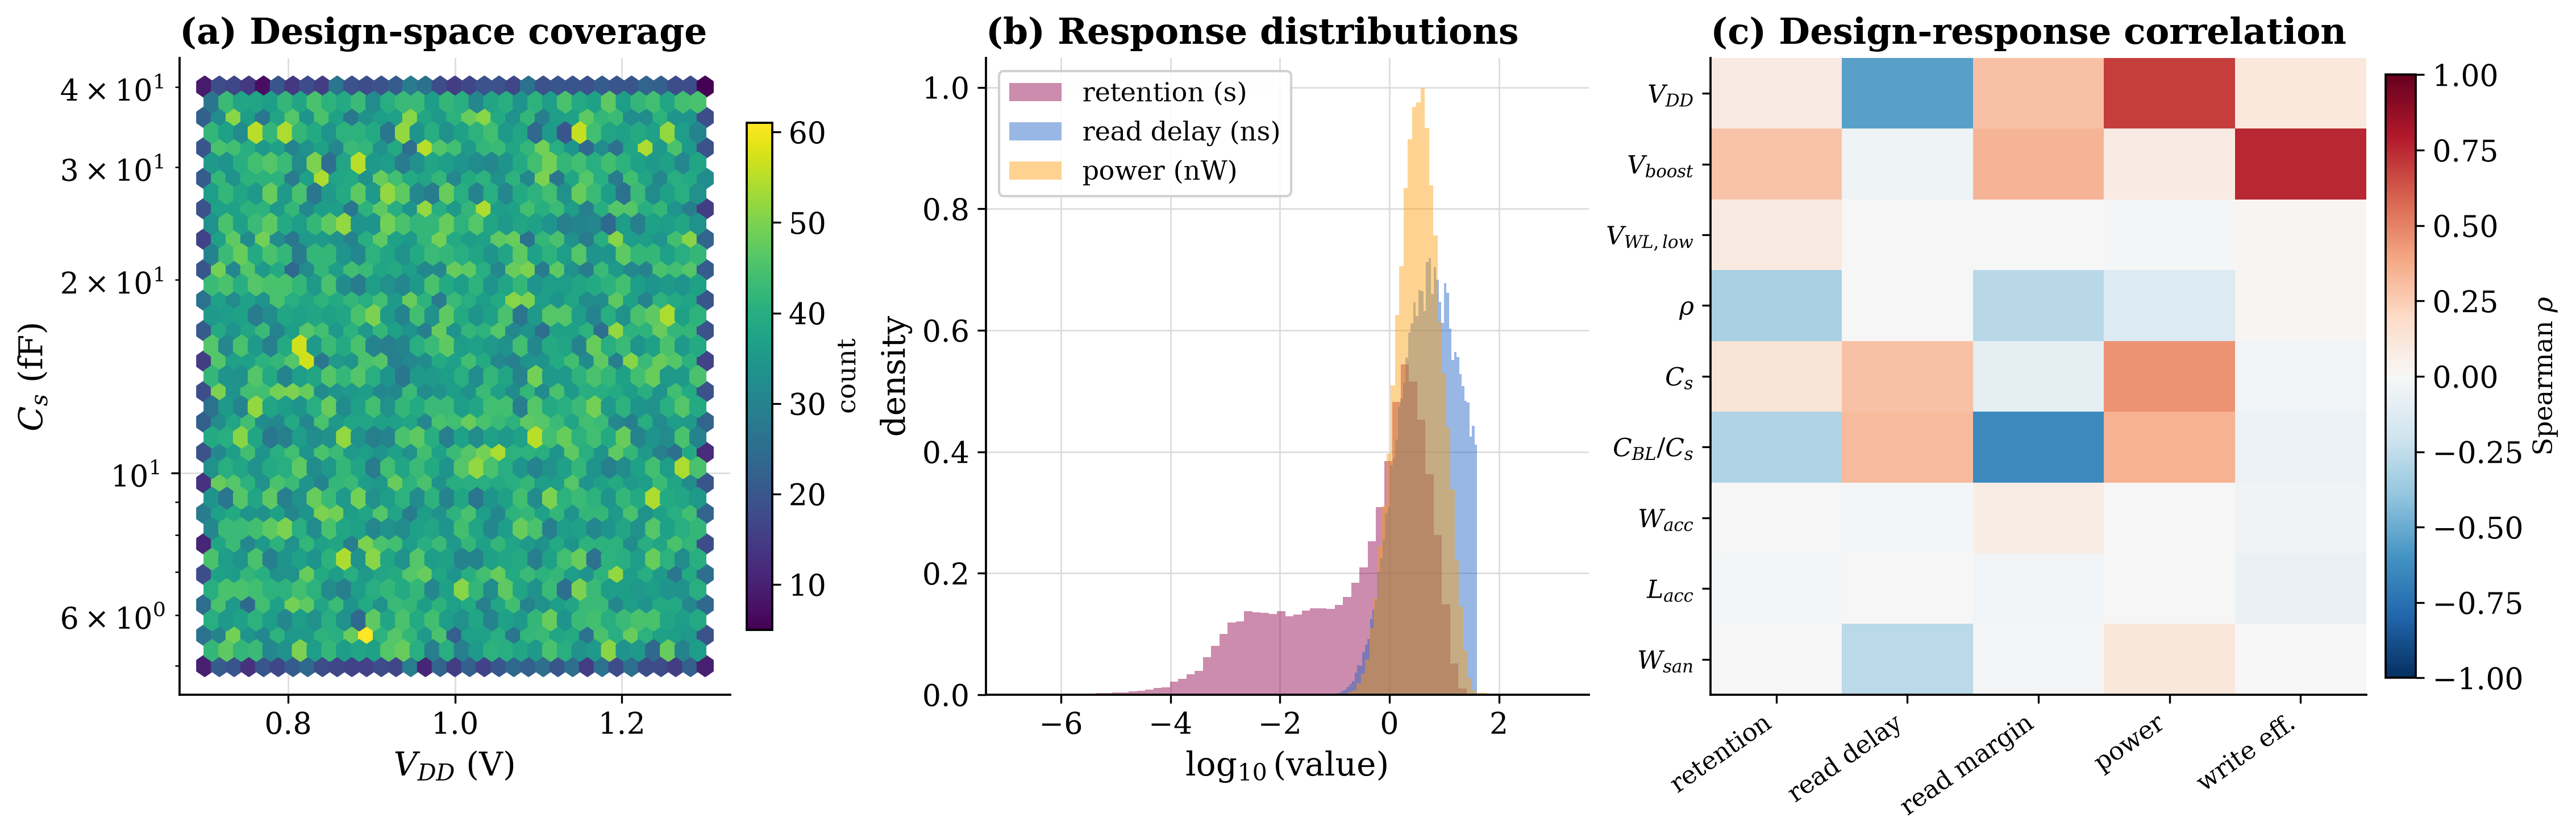
\includegraphics[width=\linewidth]{figures/fig05_dataset.png}
\caption{The released dataset. (a) Design-space coverage in the $V_{DD}$-$\Cs$
plane (hexagonal binning, $\Cs$ on a log axis). (b) The three multi-decade response
distributions, each in its own panel and native $\log_{10}$ unit. (c) Spearman
correlation between temperature and the thirteen design variables (rows) and the
responses (columns); temperature is separated at the top, and the diverging scale is
centred on zero.}
\label{fig:dataset}
\end{figure}

\begin{table}[!ht]
\centering
\caption{Composition of the released dataset. Percentiles are over all retained
rows.}
\label{tab:dataset}
\footnotesize
\begin{tabular}{@{}lrrrrr@{}}
\toprule
\textbf{Response} & \textbf{Min} & \textbf{p25} & \textbf{Median} &
\textbf{p75} & \textbf{Max} \\
\midrule
Retention time (s)        & 0      & 0.00334 & 0.341  & 2.095  & 25.83 \\
Read delay (ns)           & 0.109  & 2.195   & 5.349  & 12.70  & 39.95 \\
Read margin (mV)          & $-60.1$& 36.53   & 53.86  & 80.56  & 344.8 \\
Total power (nW)          & 0.0714 & 1.820   & 3.415  & 6.322  & 1397 \\
Storage-node leakage (fA) & 0.251  & 1.361   & 20.90  & 1032   & $1.4\times10^{7}$ \\
Write efficiency          & 0.222  & 0.816   & 0.964  & 0.989  & 0.999 \\
\midrule
\multicolumn{6}{@{}l@{}}{Rows retained / simulated: $49{,}987 / 50{,}000$;
feasible $57.9\%$; read / write success $78.6\% / 70.0\%$} \\
\multicolumn{6}{@{}l@{}}{Zero-retention points $14.5\%$; corners
9,996 to 9,998 each; train/val/test $34{,}992 / 7{,}499 / 7{,}496$} \\
\bottomrule
\end{tabular}
\end{table}

Three checks preceded use. Charge sharing matched Eq.~(\ref{eq:chargeshare}) to a
median relative error of 3.80\% (p95 17.99\%) over 120 points, the residual
reflecting junction and overlap capacitance the first-order law omits. A solver
study against a \SI{20}{\pico\second} Gear reference showed the production
\SI{50}{\pico\second} setting changing no metric by more than 0.152\% at the
median while running 1.69 times faster and preserving all pass/fail labels.
Finally the retention model was validated as in Figure~\ref{fig:retention}(d,e).

\subsection{Surrogate models and the digital twin}

Table~\ref{tab:surrogates} gives the selected model and held-out performance per
response, and Table~\ref{tab:families} the family and model comparison.
Two engineered features that are exact functions of others, the temperature in
kelvin and one capacitance-ratio duplicate, are dropped before training, since a
feature carrying no independent information only confounds later attribution; their
removal leaves accuracy unchanged. Figure~\ref{fig:parity} shows the six parity
plots: (a) retention, (b) read delay, (c) read margin, (d) power, (e) energy per
access and (f) write efficiency, each annotated with its test $R^{2}$ and RMSE.
Neural models dominate: the deep perceptron is selected for every response.
Held-out $R^{2}$ ranges from 0.951 for retention, the hardest response spanning
decades, to 0.999 for write efficiency; the wider scatter in
Figure~\ref{fig:parity}(a) at short retention is the log-floored infeasible
region.

That aggregate retention figure needs qualifying, because it is measured over a
target that is part physical and part floor. Split at the feasibility boundary, the
twin reproduces the retention of feasible designs with a median error of 0.056
decades and $R^{2}=0.73$ on the held-out set, while the floored infeasible rows,
which are easy to place near the floor but carry no gradient, inflate the aggregate
$R^{2}$ to 0.951 and dominate the RMSE. The honest reading is therefore that
retention on real, non-floored designs is predicted to within a median factor of
1.14, and that the aggregate score is optimistic. The floor is better treated as a
separate question: a gradient-boosted classifier separates feasible from infeasible
designs on the held-out set with an area under the ROC curve of 0.998 and average
precision 0.9997, so a two-stage twin, feasibility first and a feasible-only
retention regressor second, is both available and preferable to reading one
$R^{2}$ off the pooled target. Figure~\ref{fig:surrogate} summarizes the twin: (a) ranks the fourteen
models by median test $R^{2}$, placing both neural models above the boosting
family; (b) shows the selected twin per response with bootstrap intervals; and (c)
shows evaluation cost, which falls with batch size to \SI{32.5}{\micro\second} per
design at a batch of $10^{4}$, that is $30{,}769$ designs per second and a
$3.70\times10^{4}$ speedup over single-core SPICE. Two qualifications keep the
figure honest: it is the fully batched best case, an order of magnitude larger
than the tenfold speedup at batch one, and it is measured against one SPICE
process, whereas the campaign itself ran 18 workers, so the wall-clock advantage
over the parallel campaign is about $18\times$ smaller. That headroom is still what
makes the optimization, sensitivity and yield studies affordable: the optimization
alone consumes $1.68\times10^{5}$ evaluations, which the twin returns in under a
minute against about 56 hours of single-core SPICE time.

\begin{table}[!ht]
\centering
\caption{Selected surrogate per response. Selection uses the cross-validated
score; the test columns are the single untouched evaluation of that choice, with
95\% percentile-bootstrap intervals.}
\label{tab:surrogates}
\footnotesize
\begin{tabular}{@{}llrrrl@{}}
\toprule
\textbf{Response} & \textbf{Model} & \textbf{CV $R^{2}$} & \textbf{Test $R^{2}$} &
\textbf{Test RMSE} & \textbf{95\% CI} \\
\midrule
Write efficiency          & MLP (deep) & 0.99410 & 0.99917 & 0.00353 & [0.9991, 0.9993] \\
Energy per access (fJ)     & MLP (deep) & 0.99120 & 0.99666 & 2.489   & [0.9959, 0.9974] \\
$\log_{10}$ power (nW)     & MLP (deep) & 0.97042 & 0.98410 & 0.0495  & [0.9774, 0.9884] \\
Read delay (ns)           & MLP (deep) & 0.96915 & 0.98937 & 0.9616  & [0.9868, 0.9916] \\
Read margin (mV)          & MLP (deep) & 0.95378 & 0.99253 & 3.382   & [0.9905, 0.9944] \\
$\log_{10}$ retention (s) & MLP (deep) & 0.92510 & 0.95113 & 0.9197  & [0.9407, 0.9617] \\
\midrule
\multicolumn{6}{@{}l@{}}{\textit{Retention, split at the feasibility boundary
(feasible-region regression):}}\\
\quad feasible only        & MLP (deep) & --      & 0.732   & 0.674   & median err 0.056 dec \\
\quad feasibility (AUC/AP) & Hist-GBR   & --      & \multicolumn{3}{l}{AUC 0.998, AP 0.9997, accuracy 0.984} \\
\bottomrule
\end{tabular}
\end{table}

\begin{table}[!ht]
\centering
\caption{All fourteen compared models. Median test $R^{2}$ is taken across the six
responses; the mean rank averages the per-response cross-validated ranking (lower
is better). Both columns use the same aggregation.}
\label{tab:families}
\footnotesize
\begin{tabular}{@{}llrr@{}}
\toprule
\textbf{Model} & \textbf{Family} & \textbf{Median test $R^{2}$} &
\textbf{Mean rank} \\
\midrule
MLP (deep)        & Neural   & 0.9909 & 1.00 \\
MLP               & Neural   & 0.9866 & 2.33 \\
CatBoost          & Boosting & 0.9641 & 2.83 \\
LightGBM          & Boosting & 0.9595 & 4.00 \\
Hist-GBR          & Boosting & 0.9519 & 5.17 \\
XGBoost           & Boosting & 0.9544 & 5.67 \\
Poly2-ridge       & Linear   & 0.8852 & 8.00 \\
Random forest     & Ensemble & 0.8587 & 8.67 \\
GPR               & Kernel   & 0.8685 & 9.00 \\
Extra-trees       & Ensemble & 0.8665 & 9.00 \\
SVR-RBF           & Kernel   & 0.8637 & 10.33 \\
$k$-NN            & Neighbor & 0.7285 & 12.67 \\
Ridge             & Linear   & 0.6661 & 12.67 \\
Elastic-net       & Linear   & 0.6645 & 13.67 \\
\bottomrule
\end{tabular}
\end{table}

\begin{figure}[!ht]
\centering
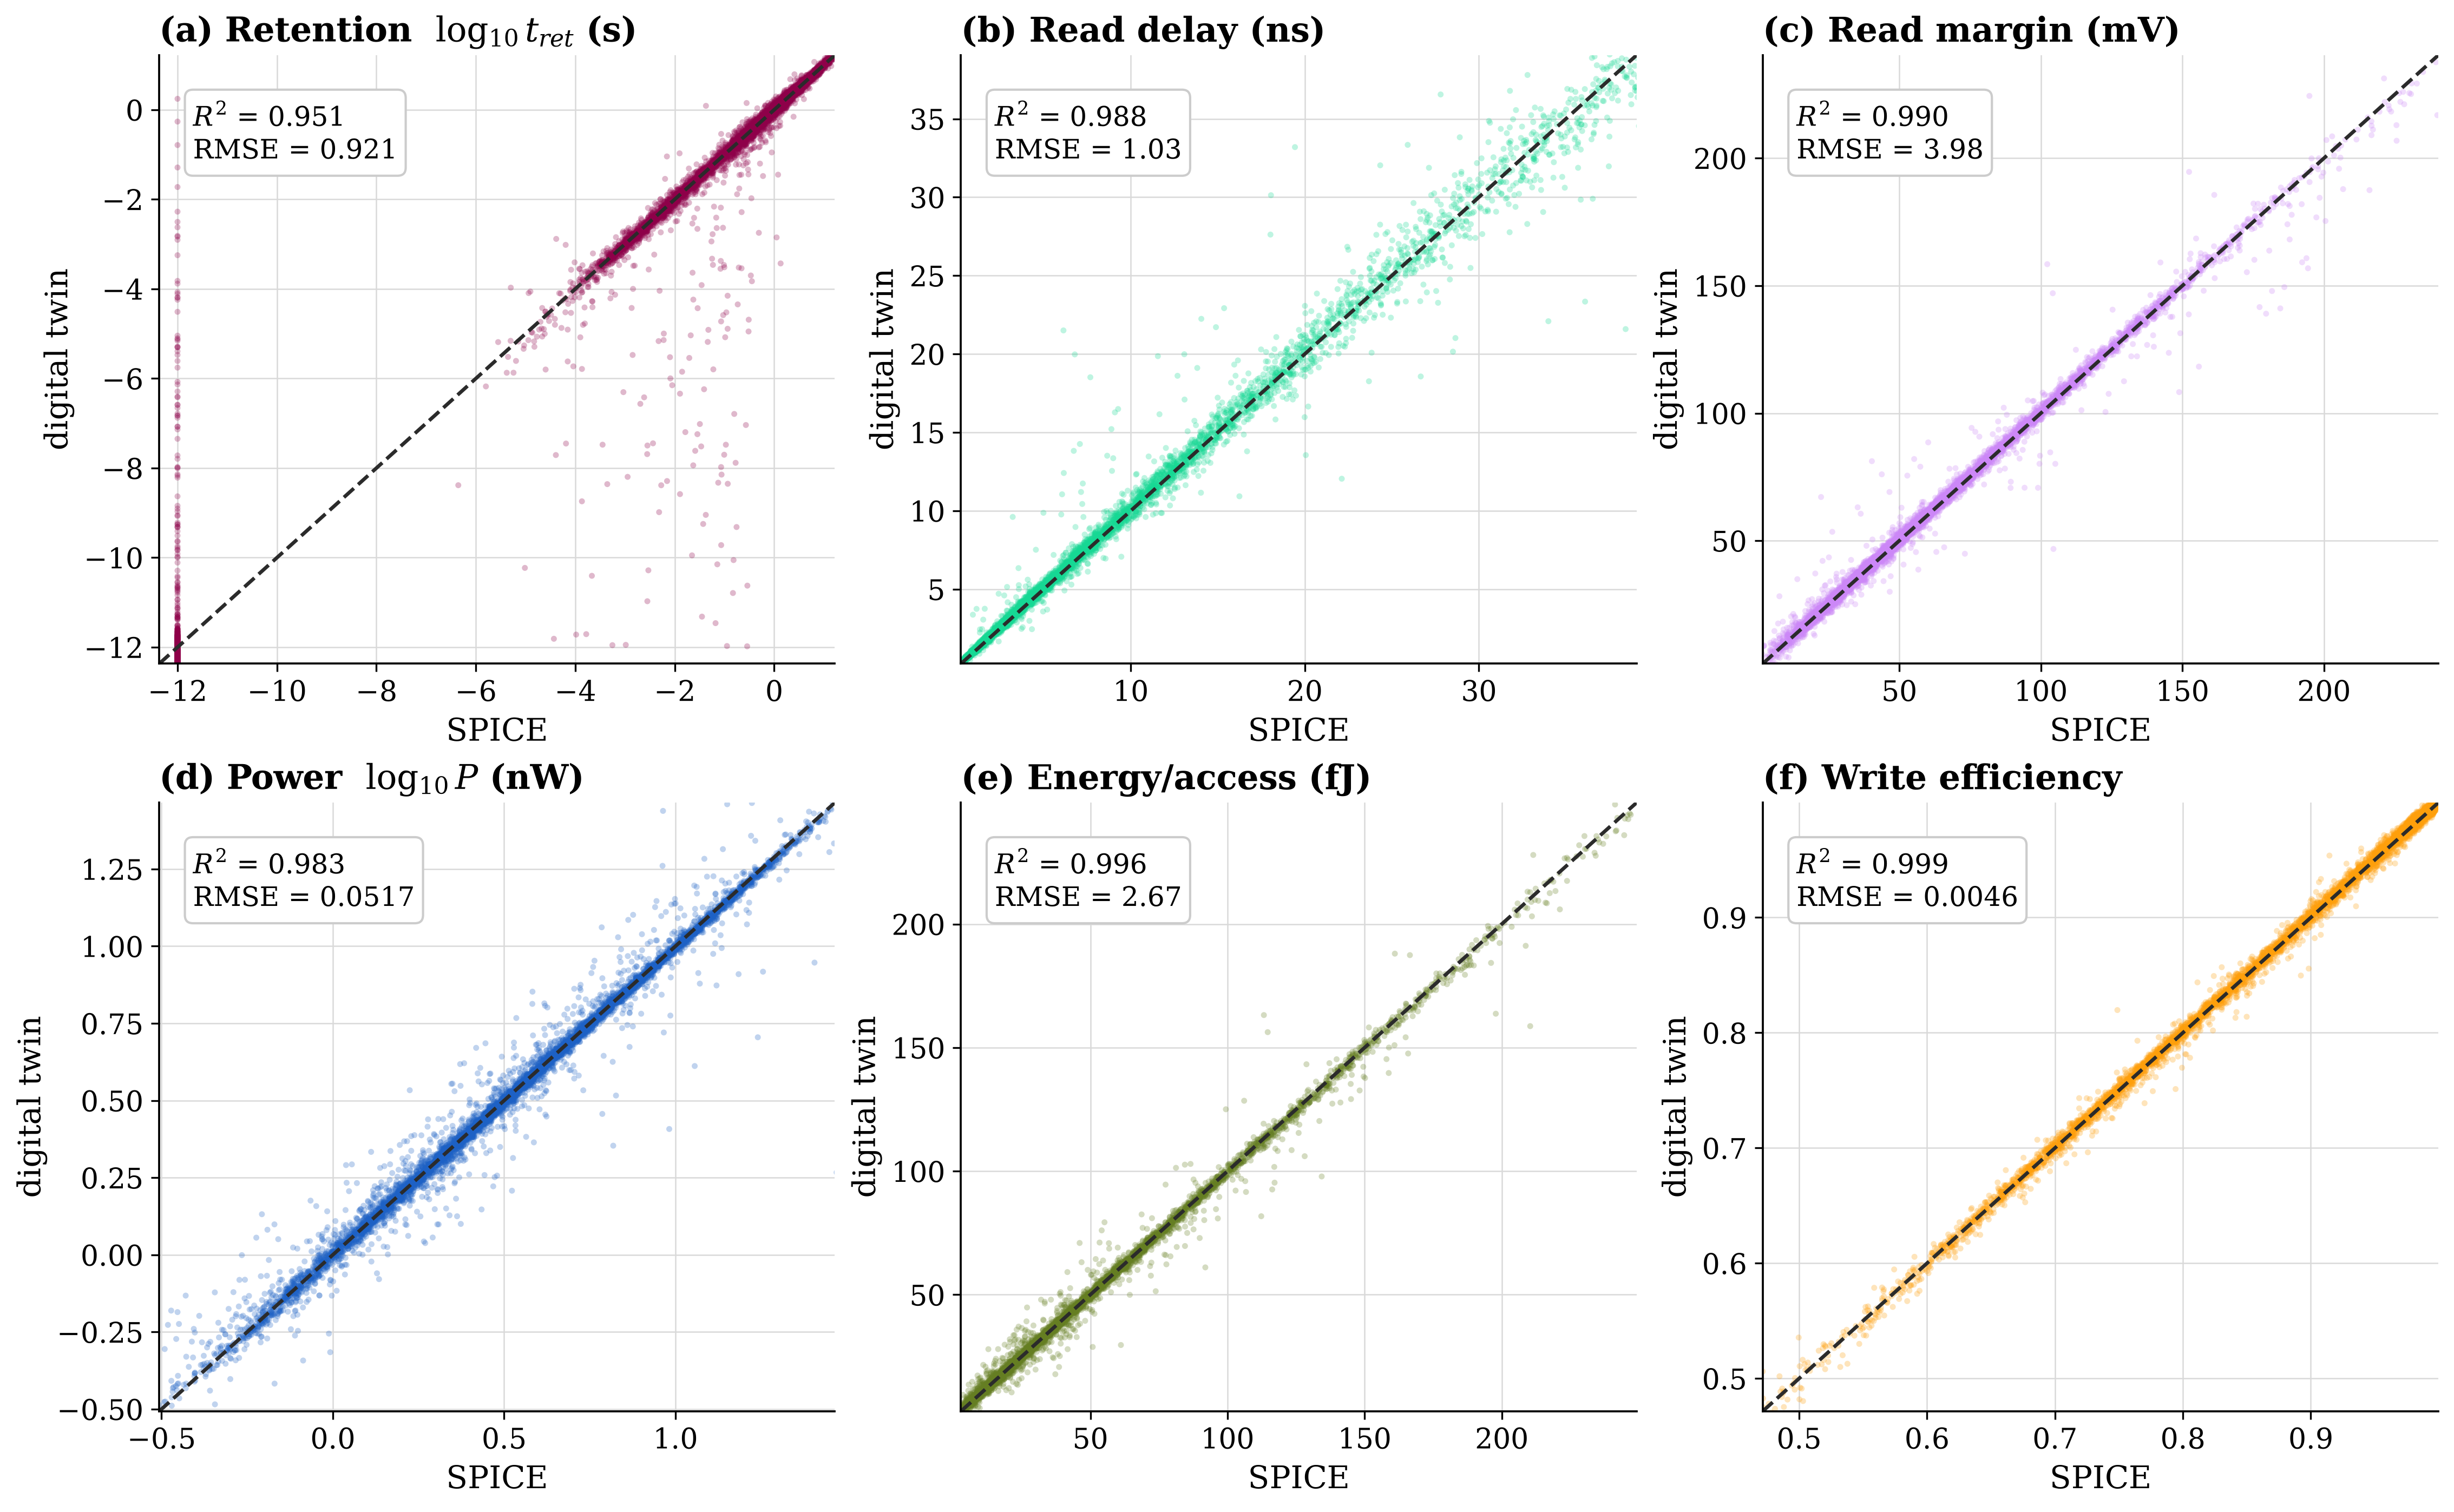
\includegraphics[width=\linewidth]{figures/fig06_parity.png}
\caption{Digital-twin predictions against SPICE on the held-out test partition
for the selected model of each response: (a) $\log_{10}$ retention, (b) read
delay, (c) read margin, (d) $\log_{10}$ power, (e) energy per access, (f) write
efficiency. Each panel is annotated with its test $R^{2}$ and RMSE; the dashed
line is the identity.}
\label{fig:parity}
\end{figure}

\begin{figure}[!ht]
\centering
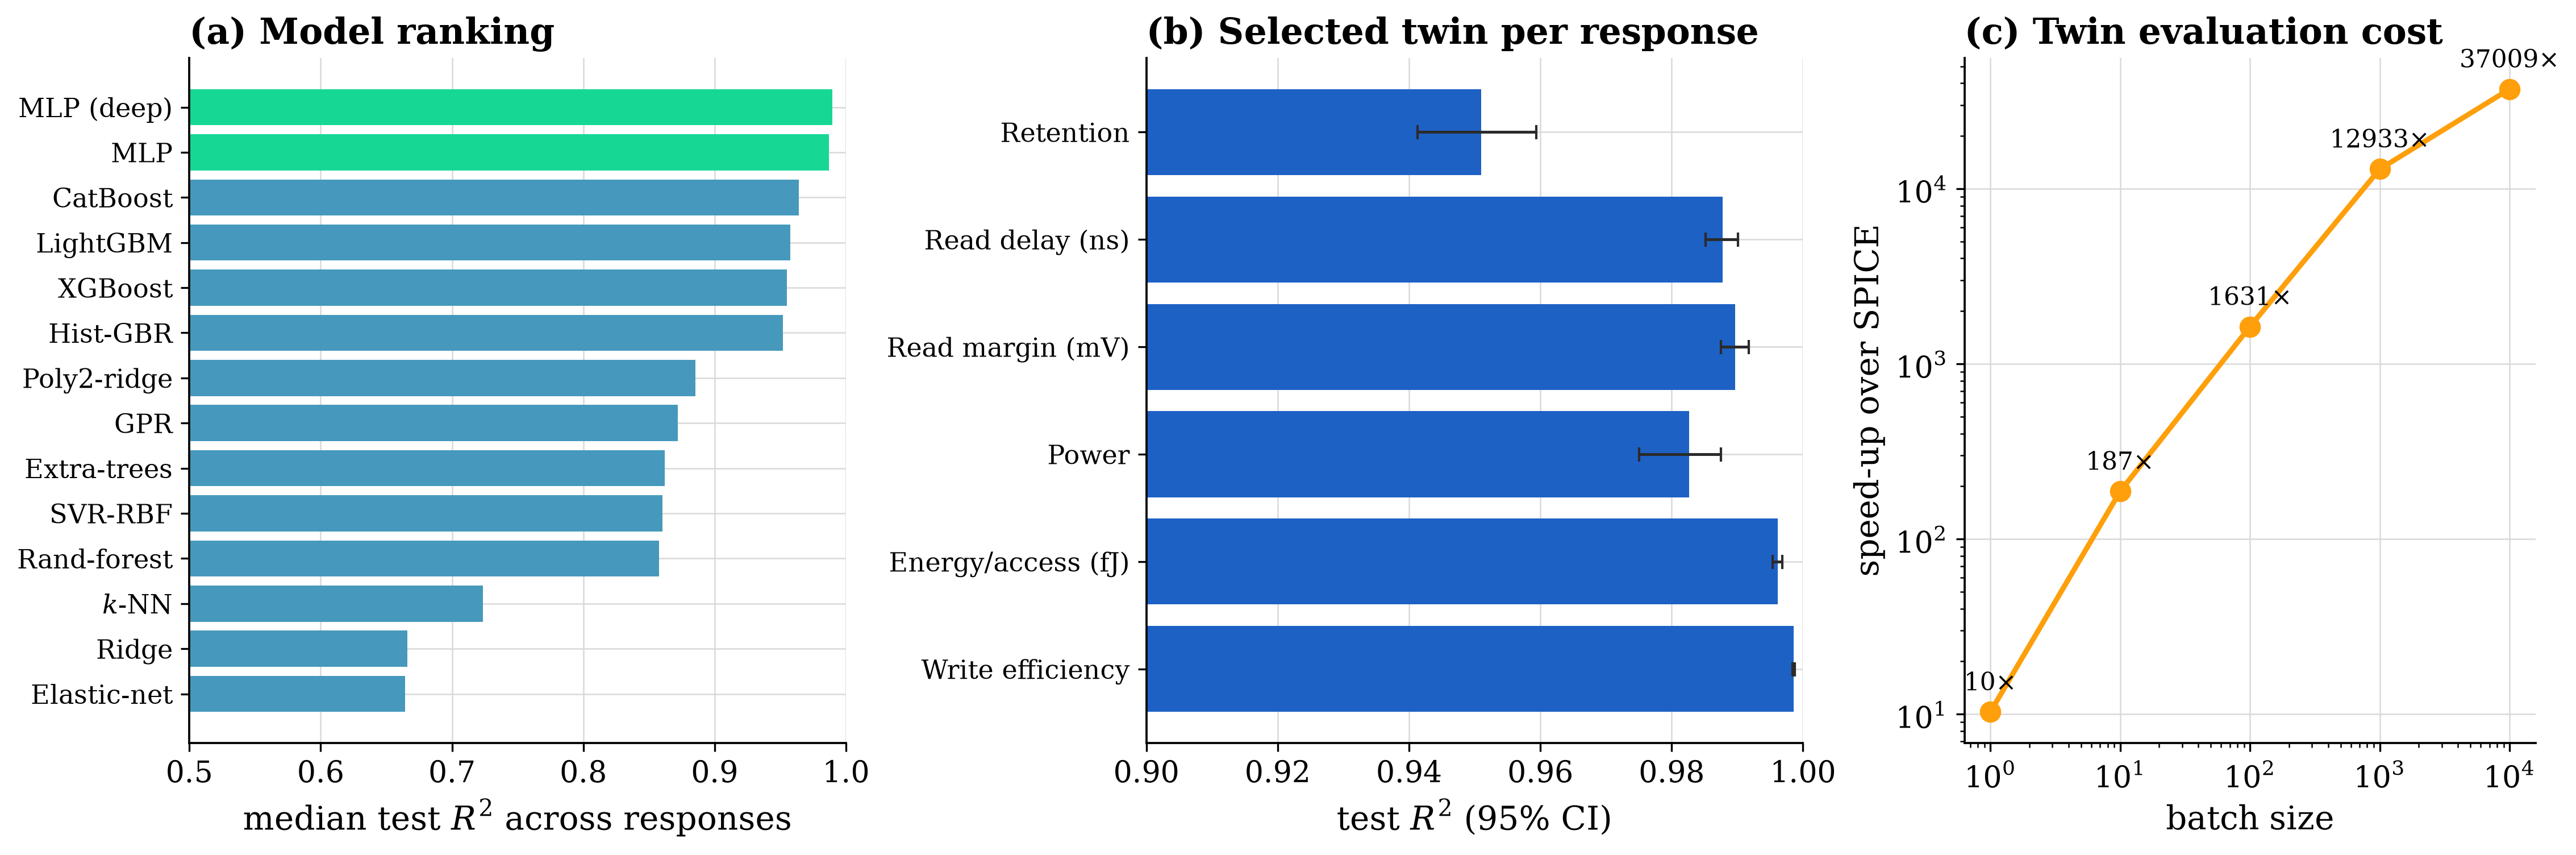
\includegraphics[width=\linewidth]{figures/fig07_surrogate.png}
\caption{Digital twin: accuracy and cost. (a) Model ranking by median test
$R^{2}$ across responses, neural models in green. (b) Selected twin per response
with 95\% bootstrap intervals. (c) Twin evaluation speedup over the measured SPICE
cost against batch size.}
\label{fig:surrogate}
\end{figure}

\subsection{Explainability}

Figure~\ref{fig:xai} interprets the twin. The two attribution methods deliberately
operate on different input spaces, and saying which is half the interpretation:
SHAP (panel~a) runs over the twin's full fifteen-feature engineered input, which
includes derived quantities such as the wordline overdrive $V_{ov}$, the gate bias
at the retention point $V_{gs,\mathrm{ret}}$ and the charge-share ratio, whereas the
Sobol' analysis of Figure~\ref{fig:robust}(c) runs over the raw design variables
alone. Panel~(a) ranks the capacitance ratio $\kappa$ first for retention, followed
by the supply, the precharge ratio $\rho$, the wordline boost and overdrive, and
temperature; colour shows that higher boost and lower precharge lengthen retention,
exactly the mechanism of Eqs.~(\ref{eq:vpp}) and~(\ref{eq:vfail}). The storage
capacitance $\Cs$ ranks lower here than a raw-variable analysis places it, because
part of its influence is carried by the derived charge-share and gate-bias features
that share its information; once the differing input spaces are accounted for, the
two analyses agree that the capacitance ratio, the precharge and supply levels, and
temperature are what govern retention. Panel~(b) aggregates attribution across all
six responses, with $V_{DD}$ the single most influential variable overall and
dominating read delay and power. Panel~(c) overlays partial dependence and
accumulated local effects for $\kappa$, both centred on a common baseline; they
agree where variables are weakly correlated and diverge for the derived ones, which
is why ALE, faithful under the correlated derived relations of
Eq.~(\ref{eq:decode}) such as $\Cbl=\kappa\Cs$ and $\Vblpre=\rho V_{DD}$, is
reported alongside.

\begin{figure}[!ht]
\centering
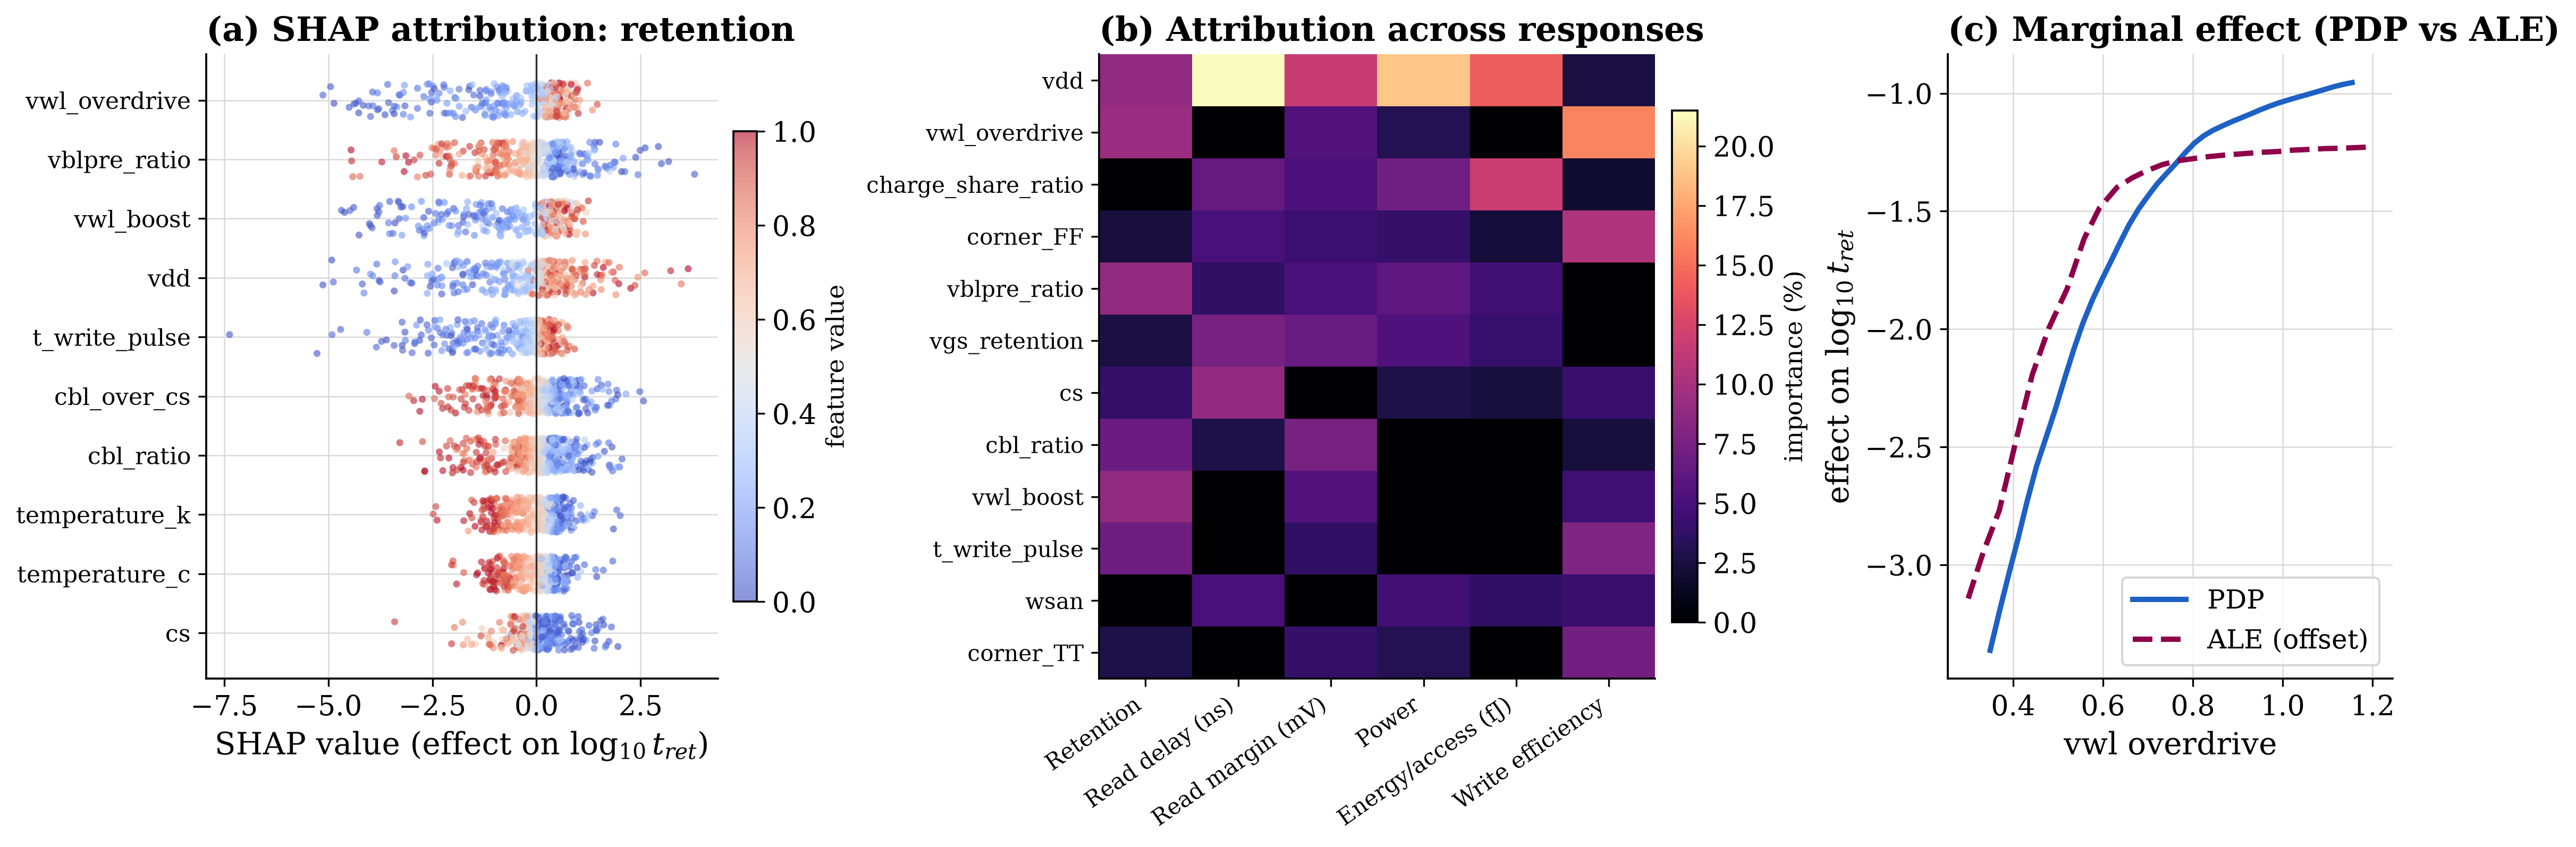
\includegraphics[width=\linewidth]{figures/fig08_xai.png}
\caption{Explainability of the twin, over the twin's fifteen-feature engineered
input. (a) SHAP summary for $\log_{10}$ retention; horizontal position is
attribution and colour is feature value. (b) Attribution (percentage) across the
six responses. (c) Marginal effect of the capacitance ratio $\kappa$, partial
dependence against accumulated local effects, both centred on a common baseline so
the comparison carries no offset.}
\label{fig:xai}
\end{figure}

\subsection{Multi-objective optimization}

Table~\ref{tab:optimizers} compares the six optimizers over 31 independent runs at
an identical 1{,}500-evaluation budget (a population of 100 over 15 generations),
with all four objectives normalized to $[0,1]$ over the pooled front and
hypervolume computed against a common reference point at 1.1 in each normalized
objective; Figure~\ref{fig:opt} visualizes the comparison. The normalization is what
makes the comparison meaningful: on the raw objectives, which span milliseconds,
nanoseconds, nanowatts and millivolts, both indicators were dominated by whichever
objective carried the largest numbers, and that alone produced the earlier
impression that a narrowly converged method could score well. Once every objective
shares a scale the ranking is unambiguous. Bayesian optimization attains the highest
median hypervolume, 0.941, then NSGA-II at 0.867 and NSGA-III at 0.768, and these
three also give the best IGD$^{+}$ (0.10, 0.11 and 0.095). The Friedman test on
hypervolume gives $\chi^2_F=144.0$, $p=2.5\times10^{-29}$, Kendall's $W=0.929$, and
with 31 runs the Nemenyi critical difference falls to 1.35 and now separates 11 of
the 15 pairs, where seven runs had separated only six, so the increased replication
is what buys the resolution. Figure~\ref{fig:opt}(d) shows the resulting structure:
Bayesian optimization and NSGA-II form the leading group and are statistically
indistinguishable, NSGA-III overlaps NSGA-II, and the two scalarizing methods with
MOEA/D trail; MOEA/D is not isolated but overlaps particle swarm. A difference is
counted significant only when it strictly exceeds the critical difference. The
MOEA/D anomaly of the raw indicators disappears under normalization: its
decomposition drives every subproblem hard but into a very narrow region of the
front, with an inter-point spacing and spread more than an order of magnitude
smaller than any other method, so it earns the worst normalized hypervolume, 0.184,
and only a middling IGD$^{+}$, 0.159, exactly as a narrowly converged front should,
not the best. The two scalarizing methods, differential evolution and particle
swarm, each pool an archive over a spread of weight vectors yet return only a
handful of well-separated optima (medians of 7 and 6), so their low hypervolume
reflects the coverage a scalarization reaches within the budget rather than a
failure of search, and they are scored on the same normalized indicators as the
rest. The Solutions column is the median size of each method's own final
non-dominated archive per run, not a share of any pooled set. Figure~\ref{fig:opt}
shows (a) the retention-versus-read-delay projection with its 2-D non-dominated
subset drawn, (b) hypervolume convergence, and (c) the hypervolume distribution by
algorithm.

\begin{table}[!ht]
\centering
\caption{Optimizer comparison over 31 runs at an identical 1{,}500-evaluation
budget, on objectives normalized to $[0,1]$ over the pooled front with the
hypervolume reference point at 1.1 in each. Hypervolume larger is better;
IGD$^{+}$ smaller is better. Statistics are on hypervolume.}
\label{tab:optimizers}
\footnotesize
\begin{tabular}{@{}lrrrrr@{}}
\toprule
\textbf{Algorithm} & \textbf{HV median} & \textbf{HV s.d.} & \textbf{IGD$^{+}$} &
\textbf{Solutions} & \textbf{Mean rank} \\
\midrule
Bayesian (TPE)              & \textbf{0.941} & 0.048 & 0.101 & 143 & \textbf{1.26} \\
NSGA-II                     & 0.867 & 0.076 & 0.107 & 100 & 1.81 \\
NSGA-III                    & 0.768 & 0.064 & \textbf{0.095} & 35 & 2.94 \\
Differential evolution      & 0.290 & 0.056 & 0.311 & 7  & 4.35 \\
Particle swarm              & 0.270 & 0.047 & 0.312 & 6  & 4.74 \\
MOEA/D                      & 0.184 & 0.028 & 0.159 & 99 & 5.90 \\
\midrule
\multicolumn{6}{@{}l@{}}{Friedman $\chi^2_F=144.0$, $p=2.5\times10^{-29}$,
$W=0.929$; Nemenyi CD $=1.35$ (11 of 15 pairs significant)} \\
\multicolumn{6}{@{}l@{}}{Leading clique (not separated): Bayesian and NSGA-II;
$n=31$ gives the pairwise tests power the seven-run study lacked} \\
\bottomrule
\end{tabular}
\end{table}

\begin{figure}[!ht]
\centering
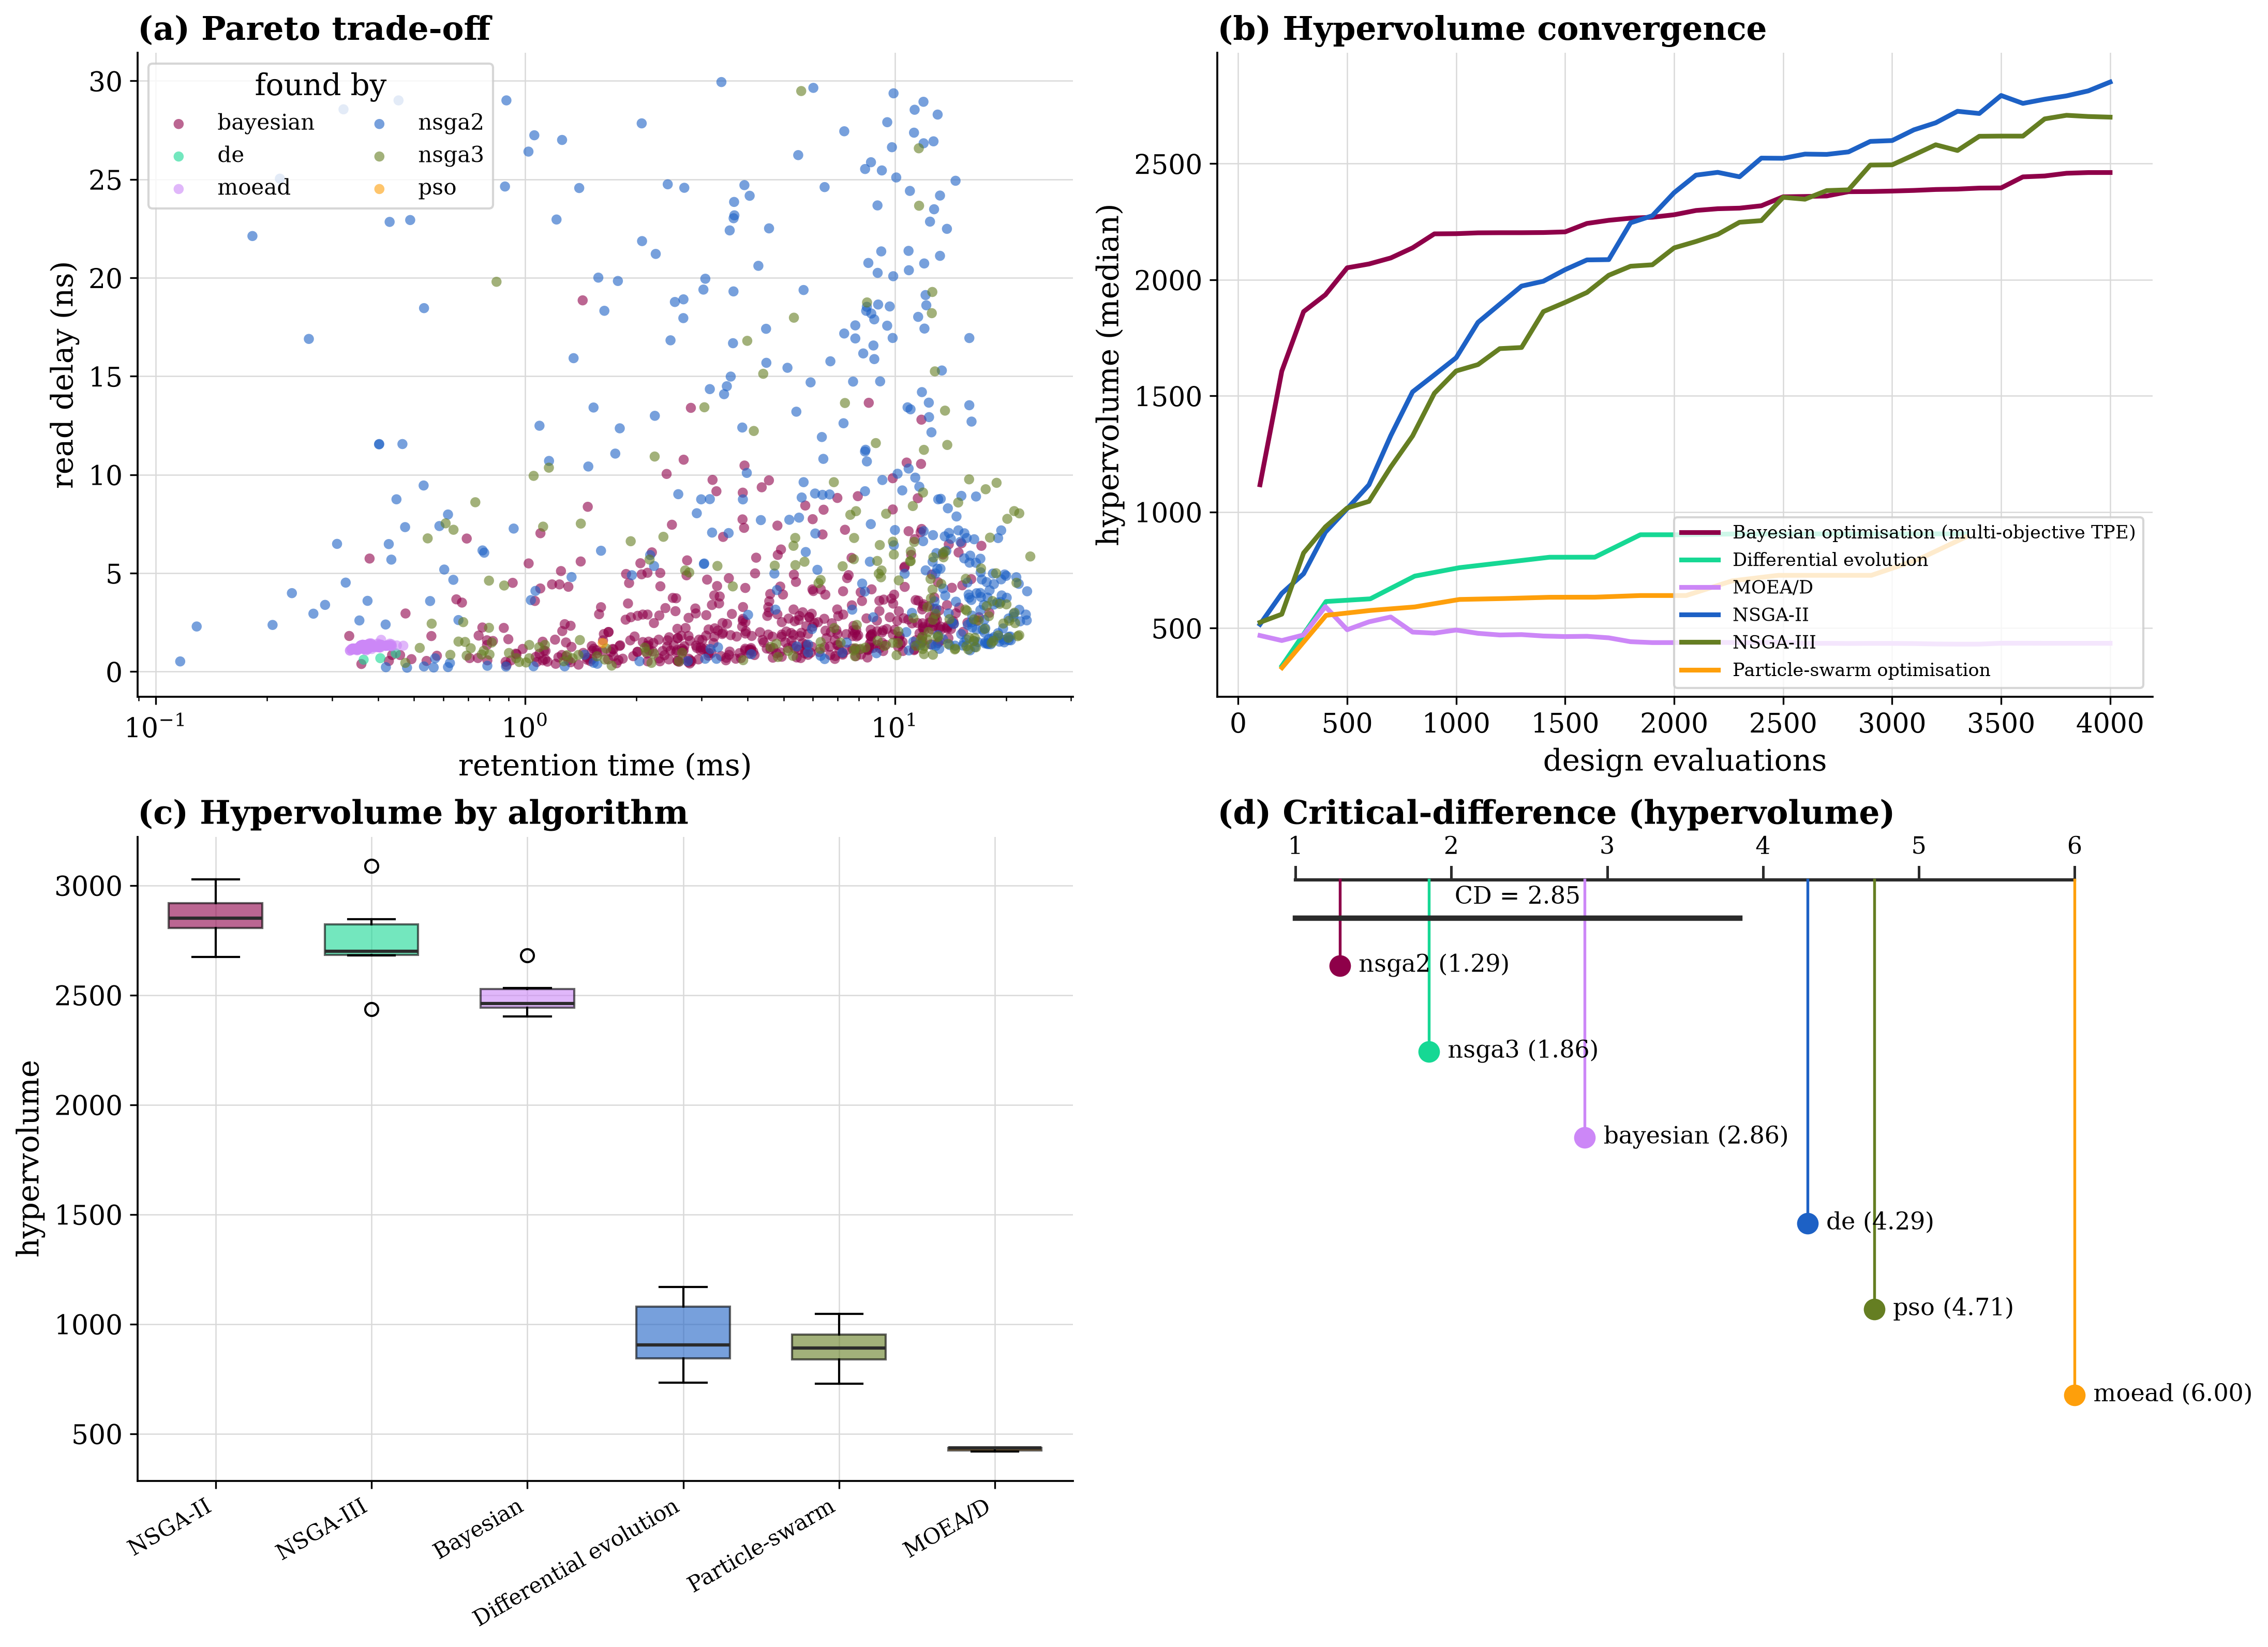
\includegraphics[width=\linewidth]{figures/fig09_optimization.png}
\caption{Multi-objective optimization over 31 runs on objectives normalized to
$[0,1]$. (a) Retention-versus-read-delay projection of the four-dimensional front,
coloured per algorithm, with the 2-D non-dominated subset drawn as the black line so
the trade-off is visible. (b) Hypervolume convergence (median over 31 runs), one
fixed colour per algorithm, legend outside the axes. (c) Hypervolume distribution by
algorithm. (d) Critical-difference diagram for hypervolume (Nemenyi,
$\mathrm{CD}=1.35$); each bar joins a clique of methods that are not significantly
different.}
\label{fig:opt}
\end{figure}

\subsection{Selected designs and SPICE verification}

Table~\ref{tab:designs} lists representative Pareto designs. A clear pattern
emerges: every high-retention design drives the capacitance ratio to its lower
bound and $\Cs$ toward its upper bound, exactly as
Eqs.~(\ref{eq:chargeshare}) and~(\ref{eq:vfail}) predict, since a light bitline
both raises charge-sharing gain and lowers the failure level.

\begin{table}[!ht]
\centering
\caption{Representative Pareto-optimal designs. Objective values are worst case
over the four PVT conditions.}
\label{tab:designs}
\footnotesize
\begin{tabular}{@{}llrrrrrrr@{}}
\toprule
\textbf{Selection} & \textbf{By} & $V_{DD}$ & $\Cs$ & $\Cbl/\Cs$ &
\textbf{$\tret$} & \textbf{$t_{rd}$} & \textbf{P} & \textbf{Margin} \\
 & & (V) & (fF) & & (ms) & (ns) & (nW) & (mV) \\
\midrule
Knee            & NSGA-II  & 1.286 & 30.2 & 2.06 & 10.33 & 2.53  & 5.94  & 230.9 \\
Weighted        & NSGA-II  & 1.163 & 39.3 & 2.00 & 12.47 & 4.14  & 6.76  & 229.4 \\
Best retention  & Bayesian & 1.269 & 39.2 & 2.37 & \textbf{14.11} & 4.51 & 8.44 & 202.1 \\
Best read delay & NSGA-II  & 1.235 & 5.0  & 2.03 & 0.61  & \textbf{0.0} & 6.95 & 140.7 \\
Best power      & NSGA-II  & 0.735 & 6.0  & 2.21 & 0.46  & 23.97 & \textbf{0.41} & 90.6 \\
Best margin     & MOEA/D   & 1.300 & 5.1  & 2.00 & 0.69  & 1.33  & 4.43  & \textbf{284.5} \\
\bottomrule
\end{tabular}
\end{table}

Returning these designs to NGSpice gives two findings that point in opposite
directions (Table~\ref{tab:verify}). First, the constraints survive: all 48
verification points satisfy the read and write criteria under full simulation, so
the optimizer's feasibility reasoning is sound. Second, the objective accuracy is
uneven at the frontier. Against the held-out test split the twin reaches
$R^{2}\ge0.95$ on every response, and on the optimizer-selected designs read margin,
power and even retention still verify well, with median discrepancies of 2.0\%,
6.7\% and 0.039 decades (a factor of $1.09$). Read delay is the exception: its
median error rises to 31.6\% and its 90th percentile to 109\%. The reason is where
the read-delay optima sit; the search pushes them against the timing feasibility
boundary, where a small change in device strength swings the latch resolution time
sharply, so the surrogate, accurate in the interior, loses precision at exactly the
edge it is driven toward. This is the concrete form the extrapolation risk takes
here, and it is measured rather than assumed.

\begin{table}[!ht]
\centering
\caption{Twin-predicted versus NGSpice-simulated performance of the selected
designs, over 48 design-condition points.}
\label{tab:verify}
\footnotesize
\begin{tabular}{@{}lrrl@{}}
\toprule
\textbf{Objective} & \textbf{Median err (\%)} & \textbf{p90 err (\%)} &
\textbf{Character} \\
\midrule
Read margin (mV)   & 2.01  & 5.78   & smooth, near-linear \\
Total power (nW)   & 6.72  & 16.19  & smooth, two decades \\
Retention time (s) & 9.4   & 27.0   & 0.039 / 0.105 decades \\
Read delay (ns)    & 31.60 & 109.35 & turns sharply at the timing boundary \\
\midrule
\multicolumn{4}{@{}l@{}}{Read and write constraints satisfied: 100\% of 48 points}
\\
\bottomrule
\end{tabular}
\end{table}

\subsection{Robustness, sensitivity and assist techniques}

Yield is estimated where cells actually fail. At the nominal condition the selected
designs all pass, so a saturated 100\% tells us nothing; the informative test
applies the Pelgrom threshold mismatch of Eq.~(\ref{eq:pelgrom}) at the worst
corner, \SI{125}{\celsius} SS, drawing an independent $\delta V_{th}$ for the access
device and both sense-amplifier pairs from $\mathcal{N}(0,\sigma_{V_{th}})$ with
$\sigma_{V_{th}}=A_{VT}/\sqrt{WL}$, and re-simulating 1{,}000 trials per design in
NGSpice; the twin does not carry $\delta V_{th}$, so this is necessarily a
deck-level check. Table~\ref{tab:yield} shows the electrical yield is then a real
distribution rather than a ceiling: the robust best-margin design holds 100\% and
the knee 93.9\%, but the low-power design, whose small access and sense transistors
give the largest per-device $\sigma_{V_{th}}$, drops to 56.6\% as its read success
alone falls to 72.7\%, and a deliberately marginal design fails almost entirely.
The retention specification is a separate axis: at \SI{125}{\celsius} no design
holds its bit for \SI{64}{\milli\second} irrespective of mismatch, the
temperature-limited shortfall discussed below, so a retention-inclusive joint yield
is zero at that corner for every design and the electrical yield is the meaningful
mismatch metric. The corner sweep, meanwhile,
exposes a conclusion the nominal condition conceals. Sustaining the JEDEC
\SI{64}{\milli\second} refresh interval requires \SI{128}{\milli\second} of
retention under the $\gamma=2$ guard of Eq.~(\ref{eq:vfail}); no design in the
Pareto set reaches that at \SI{125}{\celsius}, the best worst-case retention being
\SI{12.4}{\milli\second}, which under the same guard would support only a
\SI{6.2}{\milli\second} refresh interval. Whether that shortfall is physical or an
artifact of the general-purpose logic cards, whose access devices leak less than a
production DRAM transistor, is taken up in \S\ref{sec:discussion}; either way it is
what a worst-case-aware exploration is for, not a failure of the method.
Figure~\ref{fig:robust} shows (a) the corner sweep of the knee design on a
logarithmic colour scale, retention falling from tens of seconds cold to
milliseconds hot while the corner spread within any one temperature stays small,
the physical picture that motivates the rescoped PVT claim of \S\ref{sec:discussion}
(temperature first order, corner second order for retention); (b) the Monte-Carlo
retention distribution of the best-retention design, whose median of \SI{28.1}{\second}
sits just beyond the \SI{25.83}{\second} training maximum and is therefore flagged
as an extrapolation; and (c) the Sobol' indices for retention, where the precharge
ratio ($S_T=0.34$), the capacitance ratio ($S_T=0.32$), the storage capacitance
($S_T=0.28$) and the wordline boost ($S_T=0.20$) lead, each with a bootstrap
interval, and the gap to the first-order indices shows a substantial interaction
share. This ordering is the same set the SHAP analysis of \S\ref{sec:results}
identifies; the two differ only in where $V_{DD}$ and $\Cs$ sit, for the
input-space reason given there. Across responses the supply voltage dominates read
delay ($S_T=0.78$) and power ($S_T=0.71$), so the variable that governs retention
least among the leaders is the one that governs timing and energy most.

\begin{table}[!ht]
\centering
\caption{Mismatch yield of the selected designs, 1{,}000 Monte-Carlo trials each at
\SI{125}{\celsius} SS with an independent Pelgrom $\delta V_{th}$ per device
(Eq.~\ref{eq:pelgrom}) in NGSpice. Electrical yield requires read
margin~$\ge\SI{25}{\milli\volt}$, write efficiency~$\ge0.85$ and read
delay~$\le\SI{30}{\nano\second}$ jointly.}
\label{tab:yield}
\footnotesize
\begin{tabular}{@{}lcccr@{}}
\toprule
\textbf{Design} & \textbf{$\sigma_{V_{th}}$ acc/san/sap (mV)} &
\textbf{Read margin (mV)} & \textbf{Read success} & \textbf{Electrical yield} \\
\midrule
Best read margin      & 21.6 / 54.9 / 50.4 & $304\pm1$  & 100\%  & \textbf{100.0\%} \\
Knee                  & 64.9 / 30.5 / 30.1 & $231\pm16$ & 100\%  & 93.9\% \\
Best total power      & 54.5 / 40.7 / 35.6 & $91\pm1$   & 72.7\% & 56.6\% \\
Marginal (stress)     & 59.2 / 52.2 / 52.2 & $21\pm5$   & 12.0\% & 0.0\% \\
\bottomrule
\end{tabular}
\end{table}

\begin{figure}[!ht]
\centering
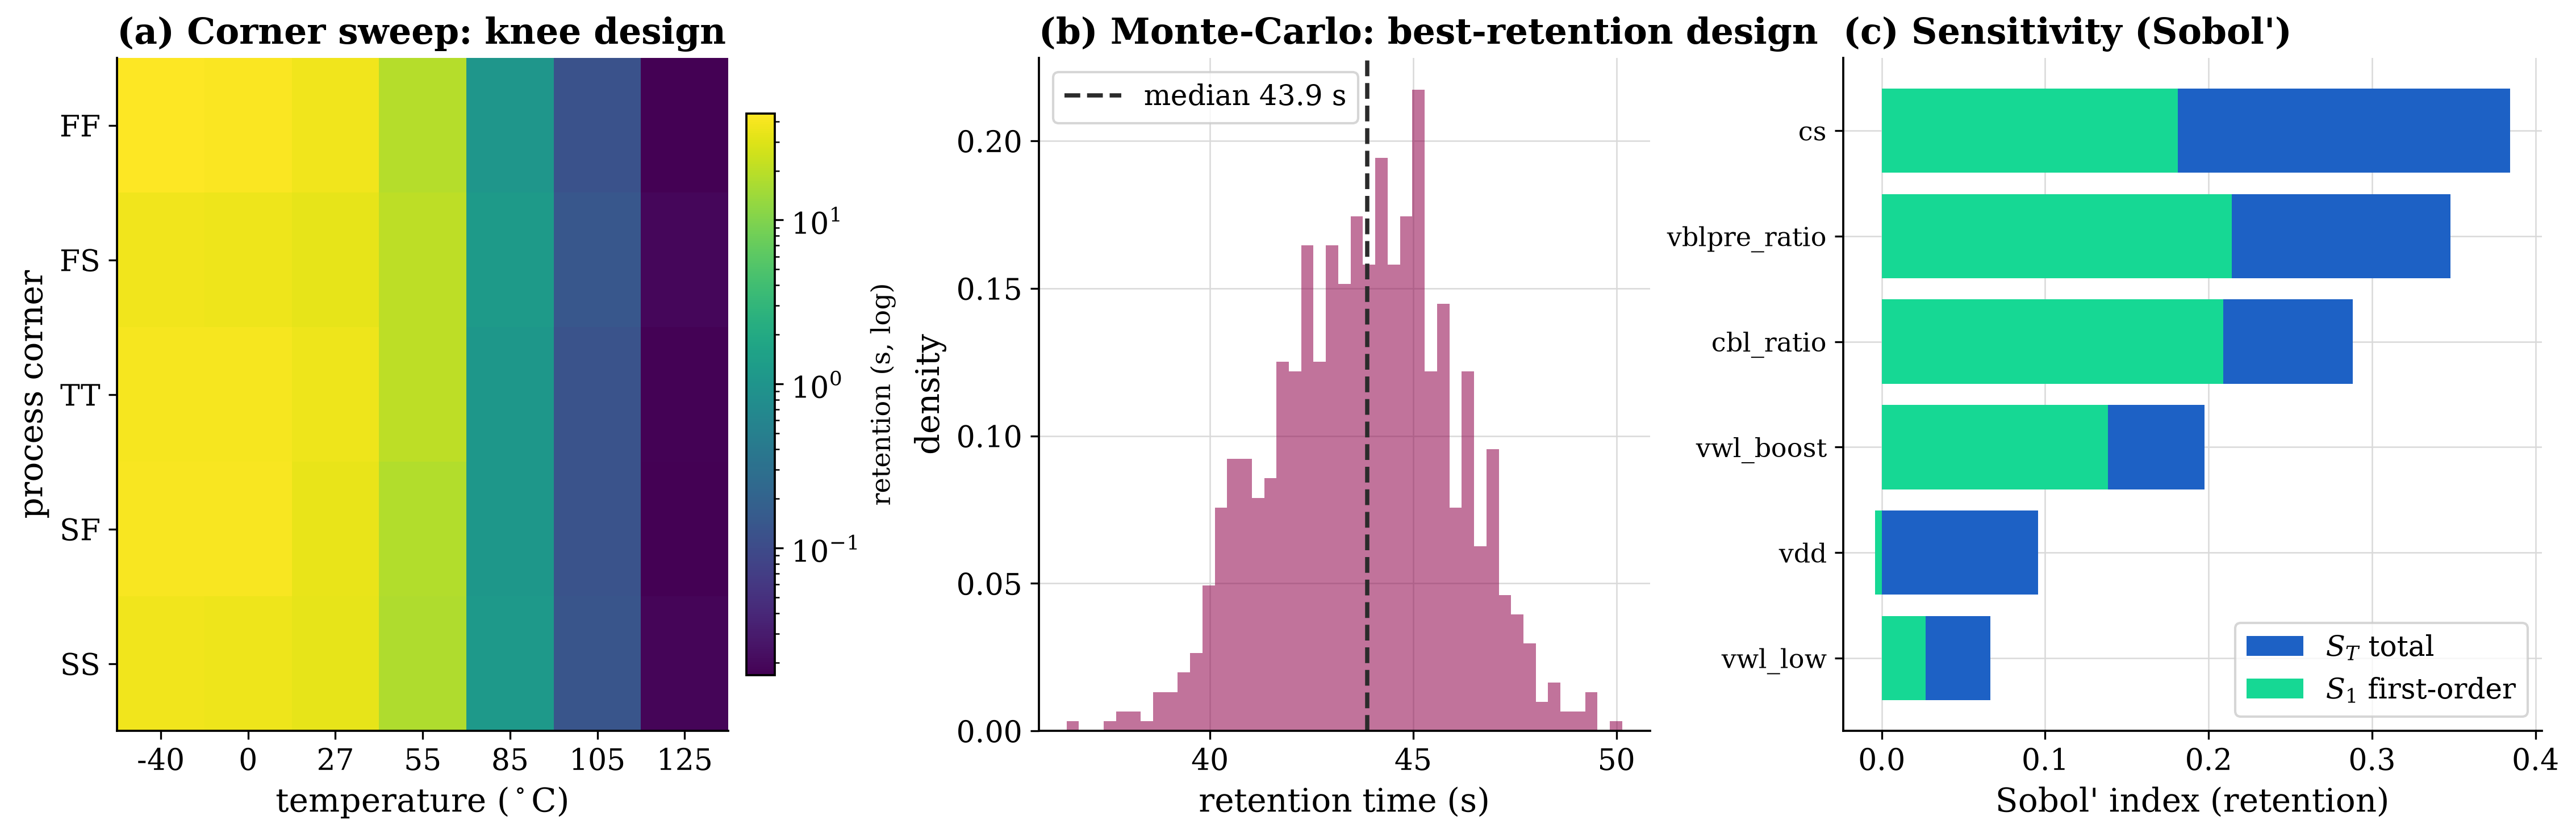
\includegraphics[width=\linewidth]{figures/fig10_robustness.png}
\caption{Robustness and sensitivity. (a) Corner sweep of the knee design across
process corner and temperature, retention on a logarithmic colour scale with the
value printed in each cell; reading down a column shows that at a fixed temperature
the corners differ only slightly, while reading across a row shows temperature
moving retention by three decades. The seven-temperature grid here is the
robustness sweep and is wider than the six-temperature characterization grid of
Figure~\ref{fig:retention}. (b) Monte-Carlo retention distribution of the
best-retention design; the dotted line marks the largest retention in the training
set and the shaded region is where the twin extrapolates beyond it. (c) Sobol'
total-effect and first-order indices for retention with bootstrap confidence
intervals; the gap between them is the interaction share.}
\label{fig:robust}
\end{figure}

Figure~\ref{fig:assist} reports the assist study, a paired and controlled design in
which each technique is composed on a common baseline over 300 base designs drawn by
a separate Latin hypercube, all simulated in NGSpice. The baseline deliberately pins
the assist-relevant knobs, wordline boost, precharge level and device sizes, to
their un-assisted nominal values, which is why its feasibility is 26.3\% rather than
the 57.9\% of the free design space: the reference is intentionally weaker than an
unconstrained draw so that each technique's effect is isolated on identical designs.
The refresh-interval control, a pure scheduling policy, correctly shows exactly
\SI{0}{\percent} change on every electrical metric and is labelled as such in the
figure. All seven rows are reported, including the leakage series on which the
negative-wordline result depends. Wordline boosting is the strongest single assist,
lengthening retention by 346.7\% and margin by 55.9\% for 6.4\% more power while
raising feasibility to 76.3\%. Bitline-precharge optimization lengthens retention by
213.9\%, consistent with lowering $\Vblpre$ and hence $\Vfail$ in
Eq.~(\ref{eq:vfail}). Sense-amplifier upsizing is a timing rather than a retention
assist: it cuts read delay by 31.6\% at 12.5\% more power and leaves retention
essentially unchanged. The high-k capacitor shortens retention by 81.2\%: its
$1.8\times$ capacitance is outweighed by a dielectric leakage entered as an assumed
parallel resistance (\SI{2e13}{\ohm} against the baseline \SI{1e15}{\ohm}), an input
to the study rather than a measured quantity, so this row's magnitude reflects that
assumption. The negative wordline shortens retention by 37.0\% while raising leakage
by 1105\%: Eqs.~(\ref{eq:isub}) and~(\ref{eq:igidl}) explain it, since subthreshold
conduction is already negligible at zero bias so a more negative gate only turns on
GIDL. Finally the combined-low-power configuration, which the multi-objective search
is expected to approach, is the instructive negative result: stacking the cell,
periphery and policy assists raises leakage by more than two orders of magnitude, so
although margin improves by 70.9\% the refresh term of Eq.~(\ref{eq:power}) drives
total power up by 90.3\% and retention barely moves, a reminder that ``low-power''
assists interact and do not add.

\begin{figure}[!ht]
\centering
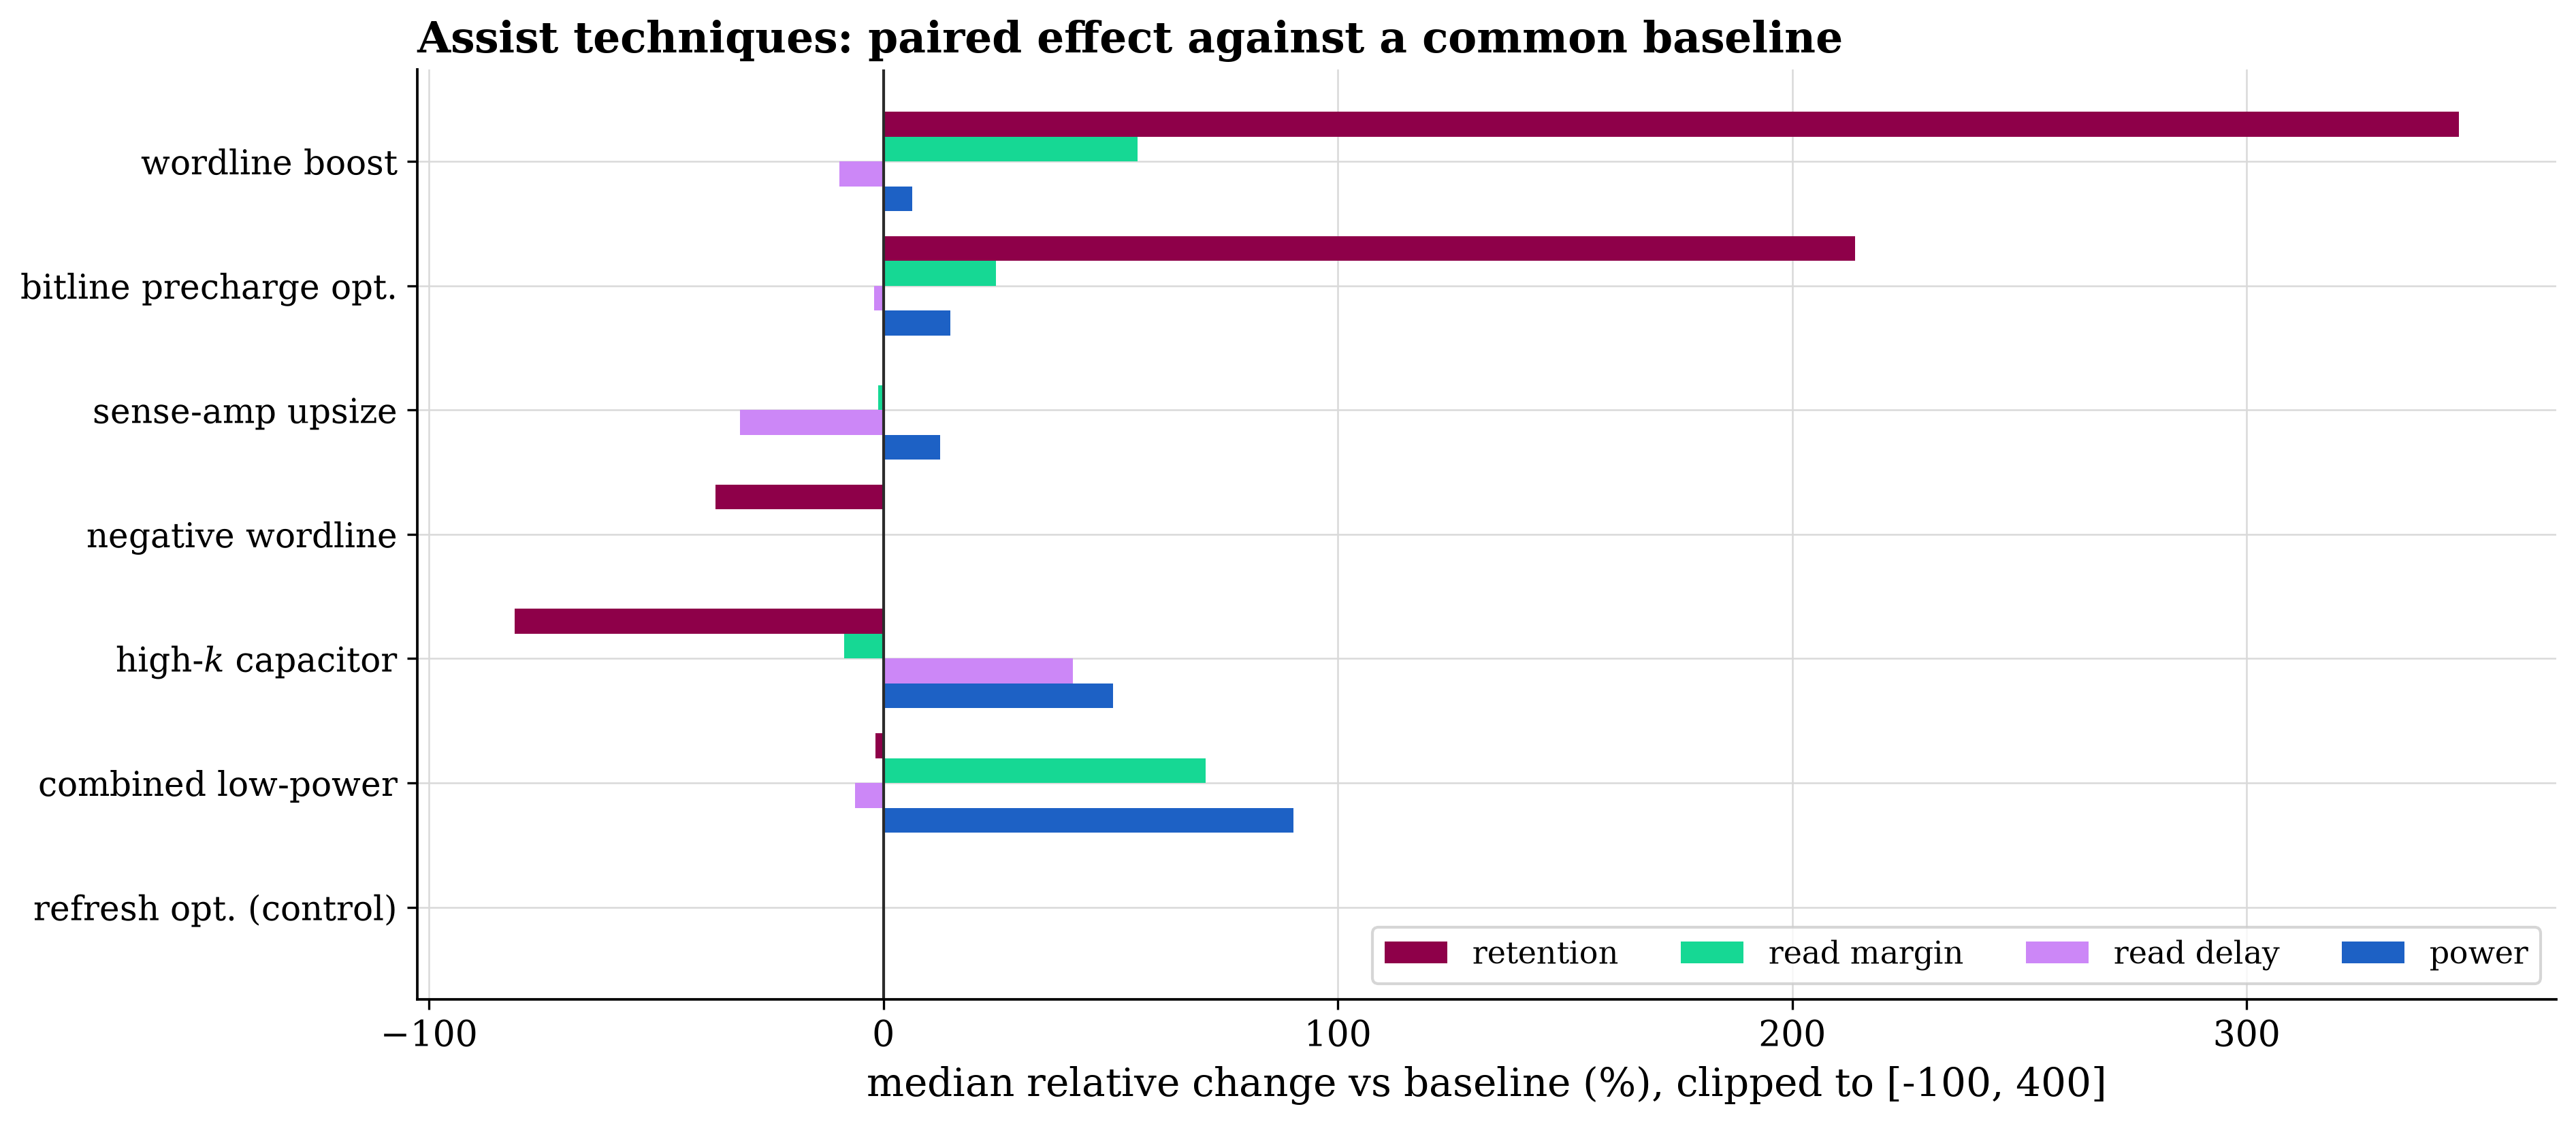
\includegraphics[width=\linewidth]{figures/fig11_assist.png}
\caption{Assist techniques as median relative change against a common baseline over
300 paired designs, all simulated in NGSpice, for five metrics including
storage-node leakage. The refresh-interval row is a null-effect control and its
zero bars are labelled explicitly. Values are clipped to $[-100, 400]\%$ for
display, with values beyond the clip annotated.}
\label{fig:assist}
\end{figure}

%=======================================================================
\section{Discussion}
\label{sec:discussion}

\subsection{Significance and relationship to existing work}

The contribution is best seen by asking what each strand of the literature would
have to do to obtain these results. Device-level retention studies
\cite{kim2021rdf,kim2021trap,bepary2022aging,park2025capleak} produce higher
physical fidelity but at a cost per point that confines them to a few devices;
this work consumes the same compact-model physics and converts it into an
observable cheap enough for 50,000 candidate designs, so the two are
complementary. Surrogate circuit-sizing methods
\cite{budak2022sizing,rashid2024global,yin2023surrogate,lberni2024eadl} share the
economics but not the obstacle: they presume the reference simulator scales, which
is false for DRAM retention, so the distinguishing contribution here is upstream
of the surrogate, in the replica construction that makes the training data
obtainable at all. Beyond that, worst-case reduction places PVT robustness inside
the loop rather than in a later check, the surrogate is chosen by a tested
fourteen-family comparison rather than asserted, and the optimizer output is
returned to the simulator with the error reported. Relative to the closest
optimizer study \cite{saglican2023moead}, the comparison is run at a replication of
31 repetitions that gives the pairwise tests real power: the Friedman omnibus and
the Nemenyi post-hoc agree, separating 11 of the 15 pairs and placing Bayesian
optimization and NSGA-II in a single leading clique that the two scalarizing methods
and MOEA/D sit well below. Relative to operational
digital twins \cite{ruhe2023dtwin,massaro2025dtwin}, this is a design-stage twin
whose value is measured by simulator agreement, which is why
Table~\ref{tab:verify} is a central result rather than an appendix. These
properties, a measured retention observable validated against the simulator, a
released dataset, statistically tested model selection, robust optimization, and a
quantified account of surrogate failure at the frontier, together make the
framework suitable as a reusable, reproducible basis for data-driven DRAM design.

\subsection{Limitations}

\begin{enumerate}
\item \textbf{Logic device models:} All simulations use public PTM BSIM4 cards for
a general-purpose low-power logic process \cite{zhao2006ptm}. Real DRAM access
devices have stronger storage-node GIDL, so the absolute retention times here are
longer than a production part; relative trends, variable rankings and the
methodology are unaffected, but no absolute retention value should be read as a
prediction about a commercial device.
\item \textbf{Access-device leakage only:} The replica is an access device driven
at the storage node (Fig.~\ref{fig:circuit}), so it captures every path the
access-device compact model carries but not dielectric leakage of the storage
capacitor, an established retention mechanism \cite{park2025capleak}. Retention here
is thus an access-device-limited estimate, and the high-$k$ assist result is driven
by an assumed dielectric-leakage multiplier rather than a measured one. Beyond the
quasi-static assumption, Eq.~(\ref{eq:tret}) also takes $\Cnode$ as
voltage-independent and treats the driven replica node as equivalent to the real
floating node; the former is the likely source of the small systematic bias in
Fig.~\ref{fig:retention}(e).
\item \textbf{Synthesized corners:} The SS/FF/SF/FS cards are first-order shifts
(Eq.~\ref{eq:corner}), spanning a defensible range but not foundry-qualified;
corner-dependent conclusions inherit this. The corner also enters the responses
unevenly: it moves read delay and read margin at first order (the sense-amplifier
strength tracks the device corner directly) but retention only weakly and mostly
through the written level, because at $V_{WL,\mathrm{low}}\le0$ the subthreshold
path is off and the GIDL and junction terms that set leakage are largely
threshold-independent. Temperature, not corner, is the first-order variable for
retention; the worst-case reduction is over both, but the retention component of it
is driven by the hot conditions.
\item \textbf{Quasi-static retention:} Equation~(\ref{eq:tret}) is exact for an
isolated capacitor with voltage-only leakage and is validated in
Figure~\ref{fig:retention}, but does not capture variable-retention-time or
trap-assisted transient behavior \cite{kim2021trap,kim2021rdf}.
\item \textbf{Lumped bitline:} $\Cbl$ is a single capacitance, so bitline
resistance, neighbor coupling and position-dependent effects are not
represented.
\item \textbf{Slice-level power:} Power is reported per cell-plus-column slice and
depends on the configured access rate; the three components are reported
separately so results can be reweighted.
\item \textbf{Frontier and out-of-range extrapolation:} As Table~\ref{tab:verify}
shows, twin accuracy on optimizer-selected designs is worse than on a random split.
A related risk is range: the best-retention designs are driven to cold corners where
the predicted retention exceeds the largest value in the training set
(\SI{25.83}{\second}, Table~\ref{tab:dataset}), so those figures are extrapolations
and are flagged as such on Fig.~\ref{fig:robust}. The twin is a search accelerator
whose proposals require confirmation; closing the loop by re-simulating the Pareto
region and refitting is the natural next step and is not done here.
\item \textbf{Statistical power and scope:} With 31 runs the pairwise post-hoc
tests resolve the ranking, but Bayesian optimization and NSGA-II remain within one
critical difference of each other, so their order is a tie rather than a ranking. A
single node (45\,nm) was carried end to end, though the pipeline is node-agnostic.
\end{enumerate}

%=======================================================================
\section{Conclusion}
\label{sec:conclusion}

This paper addressed a specific obstacle that has kept DRAM bit-cell design outside
the reach of data-driven exploration: retention time, the response that matters
most, is the one a circuit simulator cannot afford to produce in quantity because a
faithful transient spans up to ten decades of time. The resolution was to stop
simulating the discharge and instead measure what causes it. A leakage replica
embedded in the cell's own deck makes the storage-node leakage characteristic
observable in a single DC sweep, at each design point's temperature, bias and
corner, with every access-device leakage mechanism present. Retention then follows
from the exact charge-loss relation by closed-form integration, with the failure
level derived from the charge-sharing condition. Validated against direct transient
simulation across its full working range, from microseconds to twenty-five seconds,
the model reproduced the simulator with a correlation of 0.99992 in logarithmic
space and agreement within a factor of two for every matched design.

That economy changed what became possible. Fifty thousand design points were
characterized in under an hour at a success rate above 99.99 percent, yielding a
dataset in which failing designs are retained rather than discarded. From it a
digital twin was built by comparing fourteen surrogate families under
cross-validation, reaching held-out coefficients of determination between 0.951 and
0.999 and, fully batched, evaluating a design up to thirty-seven thousand times
faster than a single simulator process. That speed made worst-case-over-corners
optimization, variance-based sensitivity analysis and mismatch yield estimation
affordable, and the resulting designs were returned to the simulator for
verification. Every selected design satisfied its read and write constraints under
nominal simulation; but subjecting them to local threshold mismatch at the worst
corner, the condition where cells actually fail, drove joint yield below one hundred
percent for the more aggressive designs, so the reported yield is a real
distribution rather than a saturated ceiling. The accuracy of the predicted
objective values held to a few percent for read margin, power and retention at the
Pareto frontier but degraded to tens of percent for read delay, whose optima sit
against the timing boundary, while the retention accuracy is itself honest only when
split at the feasibility boundary; reporting both, rather than assuming them away,
is what lets the twin be used as a search accelerator whose proposals require
confirmation. The exploration further showed that within the space
examined no design sustains the sixty-four millisecond JEDEC refresh interval at the
highest temperature, which under the retention guard band needs one hundred and
twenty-eight milliseconds of retention, a conclusion a nominal-condition study would
have missed. Two
directions follow: closing the feedback loop by re-simulating the Pareto region and
refitting, and replacing the logic-process models with process models
representative of a real DRAM technology. The framework, the dataset and every
analysis artifact are released to make both straightforward.

%=======================================================================
\section*{Data and code availability}

The framework, configuration files, the 49,987-point dataset (Excel, CSV and
Parquet), the trained digital twin, and every figure, table and run manifest are
publicly available at
\url{https://github.com/USERNAME/dram-retention-digital-twin} and are archived, on
acceptance, at Zenodo under a persistent DOI (\texttt{10.5281/zenodo.XXXXXXX}) so the
exact artifacts behind every number here can be retrieved. All randomness derives
from a single master seed through a pure (seed, label, index) hash, so results are
independent of worker count and completion order.

%=======================================================================
\begin{thebibliography}{99}
\bibitem{budak2022sizing}
Budak AF, Gandara M, Shi W, Pan DZ, Sun N, Liu B. An Efficient Analog Circuit Sizing Method Based on Machine Learning Assisted Global Optimization. IEEE Trans. Comput.-Aided Des. Integr. Circuits Syst. 2022;41:1209-1221.
\href{https://doi.org/10.1109/tcad.2021.3081405}{https://doi.org/10.1109/tcad.2021.3081405}

\bibitem{rashid2024global}
Rashid R, Krishna K, George CP, Nambath N. Machine learning driven global optimisation framework for analog circuit design. Microelectronics Journal. 2024;151:106362.
\href{https://doi.org/10.1016/j.mejo.2024.106362}{https://doi.org/10.1016/j.mejo.2024.106362}

\bibitem{yin2023surrogate}
Yin S, Wang R, Zhang J, Liu X, Wang Y. Fast Surrogate-Assisted Constrained Multiobjective Optimization for Analog Circuit Sizing via Self-Adaptive Incremental Learning. IEEE Trans. Comput.-Aided Des. Integr. Circuits Syst. 2023;42:2080-2093.
\href{https://doi.org/10.1109/tcad.2022.3221694}{https://doi.org/10.1109/tcad.2022.3221694}

\bibitem{huang2021mleda}
Huang G, Hu J, He Y, Liu J, Ma M, Shen Z, et al. Machine Learning for Electronic Design Automation: A Survey. ACM Trans. Des. Autom. Electron. Syst. 2021;26:1-46.
\href{https://doi.org/10.1145/3451179}{https://doi.org/10.1145/3451179}

\bibitem{jang2023gnn}
Jang W, Myung S, Choe JM, Kim YG, Kim DS. TCAD Device Simulation With Graph Neural Network. IEEE Electron Device Lett. 2023;44:1368-1371.
\href{https://doi.org/10.1109/led.2023.3290930}{https://doi.org/10.1109/led.2023.3290930}

\bibitem{wang2023tcadcal}
Wang BC, Tang CX, Qiu MT, Chen W, Wang T, Xu JY, et al. A machine learning approach to TCAD model calibration for MOSFET. NUCL SCI TECH. 2023;34.
\href{https://doi.org/10.1007/s41365-023-01340-x}{https://doi.org/10.1007/s41365-023-01340-x}

\bibitem{li2025devmodel}
Li X, Wu Z, Rzepa G, Karner M, Xu H, Wu Z, et al. Overview of emerging semiconductor device model methodologies: From device physics to machine learning engines. Fundamental Research. 2025;5:2149-2160.
\href{https://doi.org/10.1016/j.fmre.2024.01.010}{https://doi.org/10.1016/j.fmre.2024.01.010}

\bibitem{liu2025sann}
Liu Y, Liu X, Zhou Y, Cao P. S-ANN: Synchronous TCAD device simulation of FinFET using Artificial Neural Network. Microelectronics Journal. 2025;159:106630.
\href{https://doi.org/10.1016/j.mejo.2025.106630}{https://doi.org/10.1016/j.mejo.2025.106630}

\bibitem{maniyar2022sidewall}
Maniyar A, Srinivas PSTN, Tiwari PK, Chang-Liao KS. Impact of Process-Induced Inclined Sidewalls on Gate-Induced Drain Leakage (GIDL) Current of Nanowire GAA MOSFETs. IEEE Trans. Electron Devices. 2022;69:4815-4820.
\href{https://doi.org/10.1109/ted.2022.3194109}{https://doi.org/10.1109/ted.2022.3194109}

\bibitem{lee2022stress}
Lee K, Kaczer B, Kruv A, Gonzalez M, Eneman G, Okudur OO, et al. Gate-Induced-Drain-Leakage (GIDL) in CMOS Enhanced by Mechanical Stress. IEEE Trans. Electron Devices. 2022;69:2214-2217.
\href{https://doi.org/10.1109/ted.2022.3154341}{https://doi.org/10.1109/ted.2022.3154341}

\bibitem{thakur2023gidl}
Thakur A, Dhiman R. Comprehensive study of gate induced drain leakage in nanowire and nanotube junctionless FETs using Si1-xGex source/drain. AEU - International Journal of Electronics and Communications. 2023;167:154668.
\href{https://doi.org/10.1016/j.aeue.2023.154668}{https://doi.org/10.1016/j.aeue.2023.154668}

\bibitem{kaushal2022ncfinfet}
Kaushal S, Rana AK. Modeling and analysis of gate-induced drain leakage current in negative capacitance junctionless FinFET. J Comput Electron. 2022;21:1229-1238.
\href{https://doi.org/10.1007/s10825-022-01930-9}{https://doi.org/10.1007/s10825-022-01930-9}

\bibitem{bashir2024btbt}
Bashir MY, Jaiswal AK, Patel SD, Sahay S. Revisiting Lateral-BTBT Gate-Induced Drain Leakage in Nanowire FETs for 1T-DRAM. IEEE Trans. Electron Devices. 2024;71:2714-2720.
\href{https://doi.org/10.1109/ted.2024.3365773}{https://doi.org/10.1109/ted.2024.3365773}

\bibitem{kwak2024gidl}
Kwak B, Lee K, Kim S, Kwon D. Suppression of Gate-Induced-Drain-Leakage Utilizing Local Polarization in Ferroelectric-Gate Field-Effect Transistors for DRAM Applications. IEEE Electron Device Lett. 2024;45:813-816.
\href{https://doi.org/10.1109/led.2024.3370592}{https://doi.org/10.1109/led.2024.3370592}

\bibitem{kim2021trap}
Kim KY, Min KK, Park BG. Trap-Induced Data-Retention-Time Degradation of DRAM and Improvement Using Dual Work-Function Metal Gate. IEEE Electron Device Lett. 2021;42:38-41.
\href{https://doi.org/10.1109/led.2020.3037640}{https://doi.org/10.1109/led.2020.3037640}

\bibitem{kim2021rdf}
Kim KY, Park BG. Effect of Random Dopant Fluctuation on Data Retention Time Distribution in DRAM. IEEE Trans. Electron Devices. 2021;68:5572-5577.
\href{https://doi.org/10.1109/ted.2021.3108743}{https://doi.org/10.1109/ted.2021.3108743}

\bibitem{bepary2022aging}
Bepary MK, Talukder BMSB, Rahman MT. DRAM Retention Behavior with Accelerated Aging in Commercial Chips. Applied Sciences. 2022;12:4332.
\href{https://doi.org/10.3390/app12094332}{https://doi.org/10.3390/app12094332}

\bibitem{park2025capleak}
Park DS, Lee EO, Lee JM, Cho E, Choi B. Suppression of Capacitor Leakage Through Thermal Budget Control in DRAM With ZrO 2 -Based Dielectrics. IEEE Access. 2025;13:35019-35028.
\href{https://doi.org/10.1109/access.2024.3502036}{https://doi.org/10.1109/access.2024.3502036}

\bibitem{du2025crdram}
Du H, Zhu H, Chen S, Kang Y. CR-DRAM: Improving DRAM Refresh Energy Efficiency With Inter-Subarray Charge Recycling. IEEE Trans. VLSI Syst. 2025;33:21-34.
\href{https://doi.org/10.1109/tvlsi.2024.3445631}{https://doi.org/10.1109/tvlsi.2024.3445631}

\bibitem{golman2021refresh}
Golman R, Nachum N, Cohen T, Giterman R, Teman A. Refresh Algorithm for Ensuring 100\% Memory Availability in Gain-Cell Embedded DRAM Macros. IEEE Access. 2021;9:105831-105840.
\href{https://doi.org/10.1109/access.2021.3099970}{https://doi.org/10.1109/access.2021.3099970}

\bibitem{nguyen2021zem}
Nguyen DT, Ho NM, Le MS, Wong WF, Chang IJ. ZEM: Zero-Cycle Bit-Masking Module for Deep Learning Refresh-Less DRAM. IEEE Access. 2021;9:93723-93733.
\href{https://doi.org/10.1109/access.2021.3088893}{https://doi.org/10.1109/access.2021.3088893}

\bibitem{gupta2021tfet}
Gupta N, Makosiej A, Shrimali H, Amara A, Vladimirescu A, Anghel C. Tunnel FET Negative-Differential-Resistance Based 1T1C Refresh-Free-DRAM, 2T1C SRAM and 3T1C CAM. IEEE Trans. Nanotechnology. 2021;20:270-277.
\href{https://doi.org/10.1109/tnano.2021.3061607}{https://doi.org/10.1109/tnano.2021.3061607}

\bibitem{zhang2022batchbo}
Zhang S, Yang F, Yan C, Zhou D, Zeng X. An Efficient Batch-Constrained Bayesian Optimization Approach for Analog Circuit Synthesis via Multiobjective Acquisition Ensemble. IEEE Trans. Comput.-Aided Des. Integr. Circuits Syst. 2022;41:1-14.
\href{https://doi.org/10.1109/tcad.2021.3054811}{https://doi.org/10.1109/tcad.2021.3054811}

\bibitem{touloupas2022locomobo}
Touloupas K, Sotiriadis PP. LoCoMOBO: A Local Constrained Multiobjective Bayesian Optimization for Analog Circuit Sizing. IEEE Trans. Comput.-Aided Des. Integr. Circuits Syst. 2022;41:2780-2793.
\href{https://doi.org/10.1109/tcad.2021.3121263}{https://doi.org/10.1109/tcad.2021.3121263}

\bibitem{chen2022highdimbo}
Chen C, Wang H, Song X, Liang F, Wu K, Tao T. High-Dimensional Bayesian Optimization for Analog Integrated Circuit Sizing Based on Dropout and gm/ID Methodology. IEEE Trans. Comput.-Aided Des. Integr. Circuits Syst. 2022;41:4808-4820.
\href{https://doi.org/10.1109/tcad.2022.3147431}{https://doi.org/10.1109/tcad.2022.3147431}

\bibitem{saglican2023moead}
Saglican E, Afacan E. MOEA/D vs. NSGA-II: A Comprehensive Comparison for Multi/Many Objective Analog/RF Circuit Optimization through a Generic Benchmark. ACM Trans. Des. Autom. Electron. Syst. 2023;29:1-23.
\href{https://doi.org/10.1145/3626096}{https://doi.org/10.1145/3626096}

\bibitem{abdollahi2024xai}
Abdollahi A, Li D, Deng J, Amini A. An explainable artificial-intelligence-aided safety factor prediction of road embankments. Engineering Applications of Artificial Intelligence. 2024;136:108854.
\href{https://doi.org/10.1016/j.engappai.2024.108854}{https://doi.org/10.1016/j.engappai.2024.108854}

\bibitem{homafar2022shap}
Homafar A, Nasiri H, Chelgani SC. Modeling coking coal indexes by SHAP-XGBoost: Explainable artificial intelligence method. Fuel Communications. 2022;13:100078.
\href{https://doi.org/10.1016/j.jfueco.2022.100078}{https://doi.org/10.1016/j.jfueco.2022.100078}

\bibitem{yun2021rowhammer}
Yun D, Park M, Bak G, Baeg S, Wen SJ. Exploitations of Multiple Rows Hammering and Retention Time Interactions in DRAM Using X-Ray Radiation. IEEE Access. 2021;9:137514-137523.
\href{https://doi.org/10.1109/access.2021.3117601}{https://doi.org/10.1109/access.2021.3117601}

\bibitem{kong2025twoT}
Kong S, Shim W. Design of 2T DRAM Cell With Surrounding Poly-Si Capacitor for Enhanced Retention and Mitigated Coupling Effect. IEEE Trans. Device Mater. Relib. 2025;25:460-464.
\href{https://doi.org/10.1109/tdmr.2025.3578692}{https://doi.org/10.1109/tdmr.2025.3578692}

\bibitem{kong2024pim1}
Hwan Kong S, Shim W. Advanced 2T0C DRAM Technologies for Processing-in-Memory-Part I: Vertical Transistor on Gate (VTG) DRAM Cell Structure. IEEE Trans. Electron Devices. 2024;71:6633-6638.
\href{https://doi.org/10.1109/ted.2024.3447612}{https://doi.org/10.1109/ted.2024.3447612}

\bibitem{kong2026threeT}
Kim K, Shim W. A novel 3T DRAM cell with depletion mode PMOS for extended retention time in processing-in-memory applications. Semicond. Sci. Technol. 2026;41:045011.
\href{https://doi.org/10.1088/1361-6641/ae544d}{https://doi.org/10.1088/1361-6641/ae544d}

\bibitem{nano2026gidl}
Ma H, Gu S, Zhai M, Liu H. Suppressing Gate-Induced Drain Leakage with an Asymmetric Gate Design in HiPco CNT FETs. Nanomaterials. 2026;16:653.
\href{https://doi.org/10.3390/nano16110653}{https://doi.org/10.3390/nano16110653}

\bibitem{tcad2026refresh}
Golman R, Cohen H, Shapiro G, Teman A. Cyclic Refresh Algorithm for Ensuring 100\% Memory Availability in Gain-Cell Embedded DRAM Macros. IEEE Trans. Comput.-Aided Des. Integr. Circuits Syst. 2026;45:4532-4543.
\href{https://doi.org/10.1109/tcad.2026.3652963}{https://doi.org/10.1109/tcad.2026.3652963}

\bibitem{ted2026refresh}
Ko K, Moon D, Kim J, Oh J, Park S, Song J. Dipole-Based Characteristic Enhancement Strategy for Refresh Performance Enhancement in DRAM BCAT Structure. IEEE Trans. Electron Devices. 2026;73:4885-4890.
\href{https://doi.org/10.1109/ted.2026.3708805}{https://doi.org/10.1109/ted.2026.3708805}

\bibitem{luza2022neutron}
Matana Luza L, Soderstrom D, Puchner H, Alia RG, Letiche M, Cazzaniga C, et al. Neutron-induced effects on a self-refresh DRAM. Microelectronics Reliability. 2022;128:114406.
\href{https://doi.org/10.1016/j.microrel.2021.114406}{https://doi.org/10.1016/j.microrel.2021.114406}

\bibitem{afacan2021review}
Afacan E, Lourenco N, Martins R, Dundar G. Review: Machine learning techniques in analog/RF integrated circuit design, synthesis, layout, and test. Integration. 2021;77:113-130.
\href{https://doi.org/10.1016/j.vlsi.2020.11.006}{https://doi.org/10.1016/j.vlsi.2020.11.006}

\bibitem{mina2022review}
Mina R, Jabbour C, Sakr GE. A Review of Machine Learning Techniques in Analog Integrated Circuit Design Automation. Electronics. 2022;11:435.
\href{https://doi.org/10.3390/electronics11030435}{https://doi.org/10.3390/electronics11030435}

\bibitem{lberni2024eadl}
Lberni A, Marktani MA, Ahaitouf A, Ahaitouf A. Analog circuit sizing based on Evolutionary Algorithms and deep learning. Expert Systems with Applications. 2024;237:121480.
\href{https://doi.org/10.1016/j.eswa.2023.121480}{https://doi.org/10.1016/j.eswa.2023.121480}

\bibitem{tang2024cnn}
Tang C, Chen X, Luo Y, Zeng Y. Automatic Optimal Design Method for Circuit Sizing Based on CNN Surrogate Model Assisted Differential Evolution Algorithm. IEEE Access. 2024;12:136238-136247.
\href{https://doi.org/10.1109/access.2024.3462952}{https://doi.org/10.1109/access.2024.3462952}

\bibitem{song2022mlsizing}
Song LY, Chou CY, Kuo TC, Liu CN, Huang JD. Machine Learning Assisted Circuit Sizing Approach for Low-Voltage Analog Circuits with Efficient Variation-Aware Optimization. ACM Trans. Des. Autom. Electron. Syst. 2022;28:1-22.
\href{https://doi.org/10.1145/3567422}{https://doi.org/10.1145/3567422}

\bibitem{ns2024pareto}
NS KS, Li P. Pareto Optimization of Analog Circuits Using Reinforcement Learning. ACM Trans. Des. Autom. Electron. Syst. 2024;29:1-14.
\href{https://doi.org/10.1145/3640463}{https://doi.org/10.1145/3640463}

\bibitem{vlsi2026transformer}
Sun M, Li H, Chen W, Li X, Li J, Luo Z, et al. Transformer-based surrogate modeling for multi-circuit analog sizing via Bayesian optimization. Integration. 2026;111:102809.
\href{https://doi.org/10.1016/j.vlsi.2026.102809}{https://doi.org/10.1016/j.vlsi.2026.102809}

\bibitem{tcad2026multitask}
Chen M, Hao Y, Gandara M, Imran M, Liu B. Trade-off-aware Analog Circuit Sizing Based on A Multitask Surrogate Model-assisted Evolutionary Algorithm. IEEE Trans. Comput.-Aided Des. Integr. Circuits Syst. 2026:1-1.
\href{https://doi.org/10.1109/tcad.2026.3677769}{https://doi.org/10.1109/tcad.2026.3677769}

\bibitem{akbar2022devsim}
Akbar C, Li Y, Thoti N. Device-Simulation-Based Machine Learning Technique for the Characteristic of Line Tunnel Field-Effect Transistors. IEEE Access. 2022;10:53098-53107.
\href{https://doi.org/10.1109/access.2022.3174685}{https://doi.org/10.1109/access.2022.3174685}

\bibitem{guo2023pinn}
Guo G, You H, Li C, Tang Z, Li O. A Physics-Informed Automatic Neural Network Generation Framework for Emerging Device Modeling. Micromachines. 2023;14:1150.
\href{https://doi.org/10.3390/mi14061150}{https://doi.org/10.3390/mi14061150}

\bibitem{liang2021esd}
Liang W, Yang X, Miao M, Loiseau A, Mitra S, Gauthier R. Novel ESD Compact Modeling Methodology Using Machine Learning Techniques for Snapback and Non-Snapback ESD Devices. IEEE Trans. Device Mater. Relib. 2021;21:455-464.
\href{https://doi.org/10.1109/tdmr.2021.3116599}{https://doi.org/10.1109/tdmr.2021.3116599}

\bibitem{yoon2023sram}
Yoon T, Jeong H. Machine Learning-Based Read Access Yield Estimation and Design Optimization for High-Density SRAM. IEEE Trans. Comput.-Aided Des. Integr. Circuits Syst. 2023;42:2618-2630.
\href{https://doi.org/10.1109/tcad.2022.3225066}{https://doi.org/10.1109/tcad.2022.3225066}

\bibitem{shaik2024sramaging}
Shaik JB, Guo X, Singhal S. Impact of Aging and Process Variability on SRAM-Based In-Memory Computing Architectures. IEEE Trans. Circuits Syst. I. 2024;71:2696-2708.
\href{https://doi.org/10.1109/tcsi.2024.3381935}{https://doi.org/10.1109/tcsi.2024.3381935}

\bibitem{touloupas2022mixedbo}
Touloupas K, Sotiriadis PP. Mixed-Variable Bayesian Optimization for Analog Circuit Sizing through Device Representation Learning. Electronics. 2022;11:3127.
\href{https://doi.org/10.3390/electronics11193127}{https://doi.org/10.3390/electronics11193127}

\bibitem{wang2022yieldbo}
Wang X, Yan C, Ma Y, Yu B, Yang F, Zhou D, et al. Analog Circuit Yield Optimization via Freeze-Thaw Bayesian Optimization Technique. IEEE Trans. Comput.-Aided Des. Integr. Circuits Syst. 2022;41:4887-4900.
\href{https://doi.org/10.1109/tcad.2022.3149723}{https://doi.org/10.1109/tcad.2022.3149723}

\bibitem{zhang2021nsga2mat}
Zhang P, Qian Y, Qian Q. Multi-objective optimization for materials design with improved NSGA-II. Materials Today Communications. 2021;28:102709.
\href{https://doi.org/10.1016/j.mtcomm.2021.102709}{https://doi.org/10.1016/j.mtcomm.2021.102709}

\bibitem{borisut2023alhs}
Borisut P, Nuchitprasittichai A. Adaptive Latin Hypercube Sampling for a Surrogate-Based Optimization with Artificial Neural Network. Processes. 2023;11:3232.
\href{https://doi.org/10.3390/pr11113232}{https://doi.org/10.3390/pr11113232}

\bibitem{phromphan2024lhs}
Phromphan P, Suvisuthikasame J, Kaewmongkol M, Chanpichitwanich W, Sleesongsom S. A New Latin Hypercube Sampling with Maximum Diversity Factor for Reliability-Based Design Optimization of HLM. Symmetry. 2024;16:901.
\href{https://doi.org/10.3390/sym16070901}{https://doi.org/10.3390/sym16070901}

\bibitem{liu2025xaimat}
Liu B, Liu P, Lu W, Olofsson T. Explainable Artificial Intelligence (XAI) for Material Design and Engineering Applications: A Quantitative Computational Framework. Int Journal of Mech Sys Dyn. 2025;5:236-265.
\href{https://doi.org/10.1002/msd2.70017}{https://doi.org/10.1002/msd2.70017}

\bibitem{lundberg2017shap}
Lundberg SM, Lee SI. A unified approach to interpreting model predictions. Advances in Neural Information Processing Systems (NeurIPS). 2017;30:4765-4774.

\bibitem{lundberg2020treeshap}
Lundberg SM, Erion G, Chen H, DeGrave A, Prutkin JM, Nair B, et al. From local explanations to global understanding with explainable AI for trees. Nat Mach Intell. 2020;2:56-67.
\href{https://doi.org/10.1038/s42256-019-0138-9}{https://doi.org/10.1038/s42256-019-0138-9}

\bibitem{apley2020ale}
Apley DW, Zhu J. Visualizing the Effects of Predictor Variables in Black Box Supervised Learning Models. Journal of the Royal Statistical Society Series B: Statistical Methodology. 2020;82:1059-1086.
\href{https://doi.org/10.1111/rssb.12377}{https://doi.org/10.1111/rssb.12377}

\bibitem{ruhe2023dtwin}
Ruhe S, Schaefer K, Branz S, Nicolai S, Bretschneider P, Westermann D. Design and Implementation of a Hierarchical Digital Twin for Power Systems Using Real-Time Simulation. Electronics. 2023;12:2747.
\href{https://doi.org/10.3390/electronics12122747}{https://doi.org/10.3390/electronics12122747}

\bibitem{massaro2025dtwin}
Massaro A. Electronic Artificial Intelligence-Digital Twin Model for Optimizing Electroencephalogram Signal Detection. Electronics. 2025;14:1122.
\href{https://doi.org/10.3390/electronics14061122}{https://doi.org/10.3390/electronics14061122}

\bibitem{mckay1979lhs}
McKay MD, Beckman RJ, Conover WJ. A Comparison of Three Methods for Selecting Values of Input Variables in the Analysis of Output from a Computer Code. Technometrics. 1979;21:239.
\href{https://doi.org/10.2307/1268522}{https://doi.org/10.2307/1268522}

\bibitem{zhao2006ptm}
Zhao W, Cao Y. New Generation of Predictive Technology Model for Sub-45 nm Early Design Exploration. IEEE Trans. Electron Devices. 2006;53:2816-2823.
\href{https://doi.org/10.1109/ted.2006.884077}{https://doi.org/10.1109/ted.2006.884077}

\bibitem{pelgrom1989matching}
Pelgrom MJM, Duinmaijer ACJ, Welbers APG. Matching properties of MOS transistors. IEEE J. Solid-State Circuits. 1989;24:1433-1439.
\href{https://doi.org/10.1109/jssc.1989.572629}{https://doi.org/10.1109/jssc.1989.572629}

\bibitem{ngspice}
Vogt H, Nenzi P, Warning D, et al. Ngspice, the open-source mixed-level / mixed-signal circuit simulator (version 46). 2024. \href{https://ngspice.sourceforge.io}{https://ngspice.sourceforge.io}

\bibitem{saltelli2010sobol}
Saltelli A, Annoni P, Azzini I, Campolongo F, Ratto M, Tarantola S. Variance based sensitivity analysis of model output. Design and estimator for the total sensitivity index. Computer Physics Communications. 2010;181:259-270.
\href{https://doi.org/10.1016/j.cpc.2009.09.018}{https://doi.org/10.1016/j.cpc.2009.09.018}

\bibitem{chen2016xgboost}
Chen T, Guestrin C. XGBoost: a scalable tree boosting system. Proceedings of the 22nd ACM SIGKDD International Conference on Knowledge Discovery and Data Mining. 2016:785-794.
\href{https://doi.org/10.1145/2939672.2939785}{https://doi.org/10.1145/2939672.2939785}

\bibitem{ke2017lightgbm}
Ke G, Meng Q, Finley T, Wang T, Chen W, Ma W, et al. LightGBM: a highly efficient gradient boosting decision tree. Advances in Neural Information Processing Systems (NeurIPS). 2017;30:3146-3154.

\bibitem{prokhorenkova2018catboost}
Prokhorenkova L, Gusev G, Vorobev A, Dorogush AV, Gulin A. CatBoost: unbiased boosting with categorical features. Advances in Neural Information Processing Systems (NeurIPS). 2018;31:6638-6648.

\bibitem{pedregosa2011sklearn}
Pedregosa F, Varoquaux G, Gramfort A, Michel V, Thirion B, Grisel O, et al. Scikit-learn: machine learning in Python. Journal of Machine Learning Research. 2011;12:2825-2830.

\bibitem{deb2002nsga2}
Deb K, Pratap A, Agarwal S, Meyarivan T. A fast and elitist multiobjective genetic algorithm: NSGA-II. IEEE Trans. Evol. Computat. 2002;6:182-197.
\href{https://doi.org/10.1109/4235.996017}{https://doi.org/10.1109/4235.996017}

\bibitem{deb2014nsga3}
Deb K, Jain H. An Evolutionary Many-Objective Optimization Algorithm Using Reference-Point-Based Nondominated Sorting Approach, Part I: Solving Problems With Box Constraints. IEEE Trans. Evol. Computat. 2014;18:577-601.
\href{https://doi.org/10.1109/tevc.2013.2281535}{https://doi.org/10.1109/tevc.2013.2281535}

\bibitem{zhang2007moead}
Qingfu Zhang, Hui Li. MOEA/D: A Multiobjective Evolutionary Algorithm Based on Decomposition. IEEE Trans. Evol. Computat. 2007;11:712-731.
\href{https://doi.org/10.1109/tevc.2007.892759}{https://doi.org/10.1109/tevc.2007.892759}

\bibitem{storn1997de}
Storn R, Price K. Differential Evolution - A Simple and Efficient Heuristic for global Optimization over Continuous Spaces. Journal of Global Optimization. 1997;11:341-359.
\href{https://doi.org/10.1023/a:1008202821328}{https://doi.org/10.1023/a:1008202821328}

\bibitem{kennedy1995pso}
Kennedy J, Eberhart R. Particle swarm optimization. Proceedings of ICNN'95 - International Conference on Neural Networks. 1995;4:1942-1948.
\href{https://doi.org/10.1109/icnn.1995.488968}{https://doi.org/10.1109/icnn.1995.488968}

\bibitem{bergstra2011tpe}
Bergstra J, Bardenet R, Bengio Y, Kegl B. Algorithms for hyper-parameter optimization. Advances in Neural Information Processing Systems (NeurIPS). 2011;24:2546-2554.

\bibitem{akiba2019optuna}
Akiba T, Sano S, Yanase T, Ohta T, Koyama M. Optuna: a next-generation hyperparameter optimization framework. Proceedings of the 25th ACM SIGKDD International Conference on Knowledge Discovery and Data Mining. 2019:2623-2631.
\href{https://doi.org/10.1145/3292500.3330701}{https://doi.org/10.1145/3292500.3330701}

\bibitem{blank2020pymoo}
Blank J, Deb K. Pymoo: Multi-Objective Optimization in Python. IEEE Access. 2020;8:89497-89509.
\href{https://doi.org/10.1109/access.2020.2990567}{https://doi.org/10.1109/access.2020.2990567}

\end{thebibliography}

\end{document}
